\documentclass{formato/UNIR}
\usepackage{pdfpages}
\usepackage{makecell}
%--- Parametros de entrada ---%
\titulo{Detección y mitigación de vulnerabilidades en microservicios Java mediante la integración de IA en pipelines CI/CD}
\autor{Marco Paúl Gutama Morocho \\
\hspace{3.35cm}Jonnathan Esteban Peñaranda Sarmiento}
\director{Dr. Oscar Sanjuan Martinez}
\fecha{10 de julio de 2025}
\ciudad{Logroño}
\universidad{Universidad Internacional de la Rioja (UNIR)}
\escuela{Escuela Superior de Ingeniería y Tecnología}
\master{Máster Universitario en Desarrollo y Operaciones (DevOps)}
\tipoTesis{Trabajo Fin de Máster}

\keywords{Palabrasclave} %Keywords en ingles
\keywordsEs{Palabras, clave} %Palabras clave en español


%--- Archivo de configuracion global ---%
\makeatletter
    \protected\def\autorv{\@author}
    \xdef\titulov{\@title}
    \xdef\masterv{\@master}
    \xdef\fechav{\@date}
    \xdef\universidadv{\@universidad}
    \xdef\escuelav{\@escuela}
    \xdef\tipoTesisv{\@tipoTesis}
    \xdef\directorv{\@director}
    \xdef\ciudadv{\@ciudad}
\makeatother

%Referencias 
\usepackage{footmisc}
\usepackage{hyperref}
\hypersetup{
    pdftitle={\titulov},
    %pdfauthor={\autorv},
    pdfsubject={\masterv},
    pdfpagemode={UseOutlines},
    bookmarksopen=true,
    bookmarksopenlevel=0,
    hypertexnames=false,
    colorlinks=true,
    pdfborder={0 0 0},
    citecolor=blue,
    linkcolor=blue,
    urlcolor=blue,
    pdfstartview={FitV},
    breaklinks=true
}

%Metadatos
\usepackage{hyperxmp}     
\AtBeginDocument{\hypersetup{pdfkeywords={\keywordsESv}}}


%Tablas (líneas horizonales toprule,bottomrule,midrule)
\usepackage{booktabs}

%Estructura del documento
\usepackage[toc,page,title,titletoc]{appendix}
\renewcommand*\appendixpagename{Apéndices}

%Idioma
\usepackage[spanish]{babel}
\addto\captionsspanish{\renewcommand{\tablename}{Tabla}}
\addto\captionsspanish{\renewcommand{\listtablename}{Índice de Tablas}}

%Color azul UNIR
\usepackage[dvipsnames]{xcolor}
\definecolor{azul}{RGB}{81, 131, 187}
\def\azul{\color{azul}}
\def\an{\bfseries\azul}

%Márgenes UNIR
\RequirePackage{geometry}
\geometry{
	paper=a4paper,  
	left=3.5cm,
	right=1.5cm,
	top=2.5cm, 
	bottom=2.5cm,
	headheight=0.75cm,
	headsep=1.5cm,
	footskip=1.5cm,
	%showframe, % Ver marcos
}
\usepackage{tabularx} % para tablas con anchos ajustables
\usepackage{booktabs} % para un diseño más limpio y profesional de las tablas
% Cabeceras y pies de página UNIR
\usepackage{lastpage}
\usepackage{fancyhdr}
\usepackage{tikz}
\pagestyle{fancy}
\patchcmd{\chapter}{\thispagestyle{plain}}{\thispagestyle{fancy}}{}{}

\fancypagestyle{mainmatter}{%
    \fancyhead{}%
    \lhead{\color{azul}M. Gutama, J. Peñaranda}%
    \chead{}%
    \rhead{\masterv}%
    \cfoot{}%
    \rfoot{\thepage\ of \getpagerefnumber{LastPage}}}

\fancypagestyle{frontmatter}{%
    \fancyhead{}%
    \lhead{\color{azul}M. Gutama, J. Peñaranda}%
    \chead{}%
    \rhead{\masterv}%
    \cfoot{}%
    \rfoot{\thepage}}

% Necesario para forzar encabezados y pies de página en la primera página de cada    
%\usepackage{etoolbox}      
\usepackage{setspace} % Espaciado entre líneas
\setstretch{1.5}
\usepackage[autostyle=true]{csquotes} % Referencias en UTF8

% Dependiendo del compilador se utilizan fuentes true type o fuentes convertidas (TFM)
\usepackage{array}
\usepackage{ifluatex,ifxetex}
\ifnum\ifluatex1\else\ifxetex1\else0\fi\fi
    =1 %
        % Fuentes comerciales TTF
    %Fuentes TFM UNIR: Arial, Georgia y Cambria
    \RequirePackage{fontspec}
    
    \setmainfont{Arial}[%
    Path=./formato/fuentes/,
    Extension=.ttf,
    UprightFont =*-Regular,
    BoldFont=*-Bold,
    ItalicFont=*-Italic,
    BoldItalicFont=*-BoldIt]
    
    \newfontfamily{\georgia}{Georgia}%
    [Path = ./formato/fuentes/,
    Extension = .ttf,
    UprightFont = *-Regular,
    BoldFont = *-Bold,
    ItalicFont =*-Italic,
    BoldItalicFont = *-BoldIt]
    
    \newfontfamily{\cambria}{Cambria}%
    [Path = ./formato/fuentes/,
    Extension = .ttf,
    UprightFont = *-Regular,
    BoldFont = *-Bold,
    ItalicFont =*-Italic,
    BoldItalicFont = *-BoldIt]
    
    \newcommand{\cambriamd}{\mdseries \cambria}
    \newcommand{\georgiamd}{\mdseries \georgia}
    \newcommand{\cambriab}{\bfseries \cambria}
    \newcommand{\georgiab}{\bfseries \georgia}

   
  
\else
    \renewcommand{\sfdefault}{arial}
\renewcommand{\familydefault}{\sfdefault}
\newcommand{\arialmd}{\usefont{T1}{arial}{m}{n}}
\newcommand{\arialb}{\usefont{T1}{arial}{b}{n}}
\newcommand{\arialit}{\usefont{T1}{arial}{m}{it}}
\newcommand{\arialbit}{\usefont{T1}{arial}{b}{it}}
\newcommand{\cambriamd}{\usefont{T1}{cambria}{m}{n}}
\newcommand{\cambriab}{\usefont{T1}{cambria}{b}{n}}
\newcommand{\cambriait}{\usefont{T1}{cambria}{m}{it}}
\newcommand{\cambriabit}{\usefont{T1}{cambria}{b}{it}}
\newcommand{\georgiamd}{\usefont{T1}{georgia}{m}{n}}
\newcommand{\georgiab}{\usefont{T1}{georgia}{b}{n}}
\newcommand{\georgiait}{\usefont{T1}{georgia}{m}{it}}
\newcommand{\georgiabit}{\usefont{T1}{georgia}{b}{it}}

\renewcommand{\mdseries}{\arialmd}
\renewcommand{\textmd}[1]{{\arial #1}}
\renewcommand{\bfseries}{\arialb}
\renewcommand{\textbf}[1]{{\arialb #1}}
\renewcommand{\itshape}{\arialit}
\renewcommand{\textit}[1]{{\arialit #1}}
\renewcommand{\normalfont}{\arialmd}
\renewcommand{\textnormal}[1]{{\arialmd #1}}


\fi

%--- Portada ---%
\renewcommand*{\maketitle}{%
    \begin{titlepage}%
        {\flushleft%
            {
\includegraphics[width=8.18cm]{./contenido/imagenes/logo-UNIR.pdf}}\par
        }%
        \vspace{1cm}
        \begin{table}[h!]
        \hyphenpenalty=10000
        \setlength\arrayrulewidth{2pt}
            \begin{tabularx}{14.5cm}{ L{0.074} !{\color{azul}\vline}  L{0.931} }
                & \\
                & \fontsize{14}{14}\selectfont \georgiab \universidadv\\
                & \\
                & \fontsize{18}{18}\selectfont \georgiab \escuelav \\
                & \\
                & \fontsize{14}{14}\selectfont  \georgiab\masterv \\
                & \\ & \\ & \\
                & \fontsize{34}{34}\selectfont \cambriamd \color{azul}   \titulov \\

            \end{tabularx}
        \end{table}
        \vspace{0.5cm}
        {\flushleft \fontsize{11}{11}\selectfont %
            \georgiab \tipoTesisv\par
                \vspace{0.5cm}
                Presentado por: \georgiamd \autorv \par
                \vspace{0.5cm}
                \georgiab Director: \georgiamd \directorv \par
                \vspace{3cm}
                {\color{azul}%
                \georgiab Ciudad: \georgiamd \ciudadv \par
                \georgiab Fecha: \georgiamd \fechav \par}
        }
    \end{titlepage}}
% COnfiguracion para imprimir codigo
\usepackage{listings}
\usepackage{xcolor}
\usepackage{lmodern} % Fuente moderna

% Configuración de listings para código
\definecolor{codegreen}{rgb}{0,0.6,0}
\definecolor{codegray}{rgb}{0.5,0.5,0.5}
\definecolor{codepurple}{rgb}{0.58,0,0.82}
\definecolor{backcolour}{rgb}{0.95,0.95,0.95}

\lstdefinestyle{mystyle}{
    backgroundcolor=\color{backcolour},   
    commentstyle=\color{codegreen},
    keywordstyle=\color{magenta},
    numberstyle=\tiny\color{codegray},
    stringstyle=\color{codepurple},
    basicstyle=\ttfamily\footnotesize,
    breakatwhitespace=false,         
    breaklines=true,                 
    captionpos=b,                    
    keepspaces=true,                 
    numbers=left,                    
    numbersep=5pt,                  
    showspaces=false,                
    showstringspaces=false,
    showtabs=false,                  
    tabsize=2,
    inputencoding=utf8,                 % <--- NUEVO
    extendedchars=true,                 % <--- NUEVO
    literate=                           % <--- NUEVO
      {á}{{\'a}}1 {é}{{\'e}}1 {í}{{\'i}}1 {ó}{{\'o}}1 {ú}{{\'u}}1
      {Á}{{\'A}}1 {É}{{\'E}}1 {Í}{{\'I}}1 {Ó}{{\'O}}1 {Ú}{{\'U}}1
      {ñ}{{\~n}}1 {Ñ}{{\~N}}1
      {¿}{{?``}}1 {¡}{{!``}}1
}

\lstset{style=mystyle}
% Se requiere el paquete \usepackage{amssymb} para \checkmark
% Se requiere el paquete \usepackage{pifont} para \ding{55}
% Se requiere el paquete \usepackage{xcolor} para los colores
\usepackage{amssymb}
\usepackage{pifont}
\usepackage{xcolor}

%---  Compilacion rapida ---%
% Para ahorrar tiempo de compilacion, comentar las secciones que no se quieran compilar
% Carácter % en frente de la sección.
\includeonly{
  contenido/TFM-00_Abstract,
  contenido/TFM-01_Introduccion,
  contenido/TFM-02_Contexto_y_estadodelarte,
  contenido/TFM-03_Objetivos_y_metodologia,
  contenido/TFM-04_Diseno_implementacion,
  contenido/TFM-05_Evaluacion_y_resultados,
  contenido/TFM-09_Conclusiones_y_trabajo_futuro,
  contenido/TFM-10_Bibliografia,
  contenido/TFM-11_Apendice_1,
%   contenido/TFM-11_Apendice_2 
}

%---------------------------------------------%
%           Inicio del documento
%---------------------------------------------%
\begin{document}
    %--- Paginas iniciales: portada,abstract,índice,lista de figuras y lista de tablas ---%. 
    \frontmatter
    \pagestyle{frontmatter}
        \maketitle          % Portada

        \clearpage
        \begin{abstract}[Resumen]
Las prácticas DevOps y las arquitecturas de microservicios aceleran el desarrollo de software, pero introducen desafíos de seguridad, creando una brecha entre la detección de vulnerabilidades y su corrección. Las herramientas tradicionales suelen generar alertas sin contexto, sobrecargando a los desarrolladores y ralentizando la mitigación.

Para resolver esto, se implementó un pipeline de DevSecOps en un entorno reproducible con Docker y Jenkins. La solución, definida como 'Pipeline como Código' en un \texttt{Jenkinsfile}, utiliza un script de Python para consultar una Inteligencia Artificial (IA) que analiza código Java, detecta vulnerabilidades y genera sugerencias de corrección detalladas. Un \texttt{Quality Gate} estricto detiene automáticamente el pipeline si se encuentran fallos críticos, previniendo despliegues inseguros.

La evaluación, realizada sobre una aplicación Java vulnerable, demostró la eficacia del sistema. El prototipo identificó correctamente vulnerabilidades críticas como Inyección SQL y Ejecución Remota de Código, y el \texttt{Quality Gate} detuvo el pipeline como se esperaba, marcando el build como \texttt{FAILURE}.

La principal contribución es la validación de un enfoque de \textbf{asistencia inteligente} para la seguridad. En lugar de una corrección automática riesgosa, el sistema empodera a los desarrolladores con conocimiento accionable para reducir el tiempo medio de remediación (MTTR). Se concluye que esta integración de la IA fomenta una cultura DevSecOps eficaz, transformando la seguridad de un obstáculo a una parte integral del desarrollo.

\par
\par\vspace{0.25cm}
\textbf{Palabras clave: } 
\noindent DevSecOps, CI/CD, Inteligencia Artificial, Análisis de Vulnerabilidades, Jenkins, Microservicios, Seguridad de Aplicaciones.
\end{abstract}


\pagebreak
%Ingles
\begin{abstract}
DevOps practices and microservice architectures accelerate software development but introduce security challenges, creating a gap between vulnerability detection and remediation. Traditional tools often generate context-poor alerts, burdening developers and slowing down mitigation.

To solve this, a DevSecOps pipeline was implemented in a reproducible environment with Docker and Jenkins. The solution, defined as 'Pipeline as Code' in a \texttt{Jenkinsfile}, uses a Python script to query an Artificial Intelligence (AI) model that analyzes Java code, detects vulnerabilities, and generates detailed remediation suggestions. A strict \texttt{Quality Gate} automatically halts the pipeline if critical flaws are found, preventing insecure deployments.

Evaluation on a vulnerable Java application demonstrated the system's effectiveness. The prototype correctly identified critical vulnerabilities like SQL Injection and Remote Code Execution, and the \texttt{Quality Gate} halted the pipeline as expected, marking the build as \texttt{FAILURE}.

The main contribution is the validation of an \textbf{intelligent assistance} approach to security. Instead of risky automated correction, the system empowers developers with actionable knowledge to reduce the Mean Time to Remediate (MTTR). We conclude that this AI integration fosters an effective DevSecOps culture, transforming security from a bottleneck into an integral part of development.


\par
\par\vspace{0.25cm}
\textbf{Keywords: } 
\noindent DevSecOps, CI/CD, Artificial Intelligence (AI), Vulnerability Analysis, Application Security, Jenkins, Microservices, Pipeline as Code.
\end{abstract}
  %Abtract
        \tableofcontents    % Índice
        \listoffigures      % Índice de imagenes
        \listoftables       % Índice de tablas
    
    %---    Cuerpo ---% 
    \mainmatter
    
    \pagestyle{mainmatter}
        %Incluir aqui todos los capitulos (carpeta contenido)
        %\begin{abstract}[Resumen]
Las prácticas DevOps y las arquitecturas de microservicios aceleran el desarrollo de software, pero introducen desafíos de seguridad, creando una brecha entre la detección de vulnerabilidades y su corrección. Las herramientas tradicionales suelen generar alertas sin contexto, sobrecargando a los desarrolladores y ralentizando la mitigación.

Para resolver esto, se implementó un pipeline de DevSecOps en un entorno reproducible con Docker y Jenkins. La solución, definida como 'Pipeline como Código' en un \texttt{Jenkinsfile}, utiliza un script de Python para consultar una Inteligencia Artificial (IA) que analiza código Java, detecta vulnerabilidades y genera sugerencias de corrección detalladas. Un \texttt{Quality Gate} estricto detiene automáticamente el pipeline si se encuentran fallos críticos, previniendo despliegues inseguros.

La evaluación, realizada sobre una aplicación Java vulnerable, demostró la eficacia del sistema. El prototipo identificó correctamente vulnerabilidades críticas como Inyección SQL y Ejecución Remota de Código, y el \texttt{Quality Gate} detuvo el pipeline como se esperaba, marcando el build como \texttt{FAILURE}.

La principal contribución es la validación de un enfoque de \textbf{asistencia inteligente} para la seguridad. En lugar de una corrección automática riesgosa, el sistema empodera a los desarrolladores con conocimiento accionable para reducir el tiempo medio de remediación (MTTR). Se concluye que esta integración de la IA fomenta una cultura DevSecOps eficaz, transformando la seguridad de un obstáculo a una parte integral del desarrollo.

\par
\par\vspace{0.25cm}
\textbf{Palabras clave: } 
\noindent DevSecOps, CI/CD, Inteligencia Artificial, Análisis de Vulnerabilidades, Jenkins, Microservicios, Seguridad de Aplicaciones.
\end{abstract}


\pagebreak
%Ingles
\begin{abstract}
DevOps practices and microservice architectures accelerate software development but introduce security challenges, creating a gap between vulnerability detection and remediation. Traditional tools often generate context-poor alerts, burdening developers and slowing down mitigation.

To solve this, a DevSecOps pipeline was implemented in a reproducible environment with Docker and Jenkins. The solution, defined as 'Pipeline as Code' in a \texttt{Jenkinsfile}, uses a Python script to query an Artificial Intelligence (AI) model that analyzes Java code, detects vulnerabilities, and generates detailed remediation suggestions. A strict \texttt{Quality Gate} automatically halts the pipeline if critical flaws are found, preventing insecure deployments.

Evaluation on a vulnerable Java application demonstrated the system's effectiveness. The prototype correctly identified critical vulnerabilities like SQL Injection and Remote Code Execution, and the \texttt{Quality Gate} halted the pipeline as expected, marking the build as \texttt{FAILURE}.

The main contribution is the validation of an \textbf{intelligent assistance} approach to security. Instead of risky automated correction, the system empowers developers with actionable knowledge to reduce the Mean Time to Remediate (MTTR). We conclude that this AI integration fosters an effective DevSecOps culture, transforming security from a bottleneck into an integral part of development.


\par
\par\vspace{0.25cm}
\textbf{Keywords: } 
\noindent DevSecOps, CI/CD, Artificial Intelligence (AI), Vulnerability Analysis, Application Security, Jenkins, Microservices, Pipeline as Code.
\end{abstract}

        \chapter{Introducción}\label{chap:introduccion}

La transformación digital ha consolidado a las arquitecturas de microservicios y las metodologías DevOps como pilares fundamentales en el desarrollo de software moderno. Esta combinación permite a las organizaciones construir aplicaciones escalables y entregar valor de forma rápida y continua. Sin embargo, esta agilidad introduce nuevos y complejos desafíos de seguridad. La adopción de microservicios, si bien popular, incrementa la superficie de ataque de las aplicaciones \cite{Zafeiropoulos2023SecurityGaps}, y la automatización inherente a los pipelines de Integración y Despliegue Continuo (CI/CD), un pilar de DevOps, a menudo introduce riesgos si no se gestiona adecuadamente \cite{NIST2024CICDSecurity}.

Frente a esta problemática, la propuesta principal de esta investigación se enfoca en una solución innovadora: la integración de modelos de Inteligencia Artificial (IA) existentes directamente en los flujos de trabajo de CI/CD. Este enfoque busca mejorar radicalmente la forma en que se detectan y tratan las vulnerabilidades en el código Java de los microservicios. Es crucial aclarar que el objetivo no es la corrección automática de código, lo cual podría ser riesgoso, sino la generación automatizada de sugerencias de mitigación contextualizadas y de alta calidad. Estas sugerencias se presentarían al equipo de desarrollo para su revisión y validación, asegurando el control humano sobre cambios críticos.

Este capítulo introduce el problema, justifica la necesidad de una solución y plantea la pregunta de investigación que guía el trabajo. Finalmente, se presenta la estructura del documento, detallando los capítulos que componen la tesis para facilitar la comprensión del proceso de investigación, desarrollo y los resultados obtenidos.

\section{Justificación del trabajo}\label{sec:justificaciontrabajo}

La adopción de arquitecturas de microservicios se ha vuelto una tendencia principal en la industria del software, motivada por la búsqueda de mayor agilidad en el desarrollo, escalabilidad independiente de los componentes y mejor resiliencia del sistema. No obstante, esta descomposición en servicios añade una complejidad importante a la gestión de la seguridad. El problema fundamental que esta tesis busca resolver es la ineficiencia y la tendencia a errores de los métodos tradicionales para identificar y corregir vulnerabilidades en el amplio y dinámico entorno de microservicios. La naturaleza distribuida de estos sistemas incrementa la superficie de ataque, y la posible diversidad de tecnologías y equipos dificulta la aplicación de políticas de seguridad uniformes.

Las causas de este problema son diversas: la velocidad que exigen los ciclos de desarrollo ágil y DevOps a menudo deja poco margen para revisiones de seguridad manuales detalladas; la complejidad propia de las interacciones entre servicios puede ocultar vulnerabilidades sutiles; y la gran escala (cientos o miles de microservicios en organizaciones grandes) hace que la supervisión manual sea impracticable. La importancia de solucionar este problema es crítica, ya que las fallas de seguridad pueden tener consecuencias graves como pérdida de datos, daño a la reputación o incumplimiento de normativas. Ignorar estas alertas debido a la sobrecarga de información no es una opción, sino un riesgo latente que este trabajo busca mitigar.

La motivación principal de este trabajo nace de reconocer el potencial de la Inteligencia Artificial para enfrentar estos desafíos. La capacidad de los modelos de IA actuales para analizar grandes volúmenes de código, identificar patrones de vulnerabilidades y generar sugerencias de código coherentes ofrece una oportunidad única. Integrar esta capacidad en los pipelines CI/CD es un paso lógico hacia un enfoque de seguridad más inteligente y proactivo (DevSecOps). Por lo tanto, la contribución principal de esta tesis es el diseño, implementación y validación de un sistema modular que integra IA en pipelines CI/CD para generar sugerencias de mitigación de vulnerabilidades, buscando superar las limitaciones de las herramientas tradicionales en cuanto a contexto y accionabilidad.

Adicionalmente, se busca que la solución propuesta sea de código abierto, ofreciendo una alternativa a las herramientas comerciales existentes que pueden tener un alto costo \cite{ghas_docs, sonarqube_editions} o a las versiones comunitarias con funcionalidades limitadas. Un diferenciador clave del prototipo es su diseño modular, que permitirá al usuario seleccionar el modelo de IA subyacente, adaptando así la solución a diferentes contextos de presupuesto y privacidad.

\section{Planteamiento del problema}\label{sec:planteamiento_problema}

En el ciclo de vida actual del desarrollo de software, especialmente en organizaciones que utilizan DevOps y microservicios Java, se observa una importante brecha operativa. Existe una necesidad urgente de mecanismos que no solo detecten vulnerabilidades de forma temprana y continua (aplicando el principio "Shift Left"), sino que también ofrezcan a los equipos de desarrollo una guía clara, contextualizada y fiable para su corrección, integrada de forma fluida en sus flujos de trabajo automatizados.

Las soluciones actuales, aunque han progresado, presentan limitaciones. Las herramientas de Análisis Estático de Seguridad (SAST), si bien son esenciales, frecuentemente generan un gran volumen de alertas, incluyendo una cantidad significativa de falsos positivos. Este "ruido" dificulta la priorización, consume tiempo valioso de los desarrolladores y puede llevar a una "fatiga de alertas" que reduce la confianza en la herramienta \cite{Johnson2023UsabilitySAST}. La clasificación de estas alertas y la investigación de la mitigación adecuada sigue siendo un proceso manual intensivo, actuando como un cuello de botella que ralentiza el ciclo de retroalimentación.

Para responder a esta necesidad, se propone desarrollar un sistema que utiliza modelos de Inteligencia Artificial (IA) para el análisis integral de código, integrado como una etapa dentro del pipeline CI/CD. La finalidad de esta tesis es diseñar, construir y evaluar un prototipo funcional de este sistema. El prototipo enviará el código fuente a un modelo de IA seleccionado para un análisis exhaustivo que no solo identificará vulnerabilidades, sino que también evaluará la calidad general del código. Para validar su eficacia, los resultados se compararán con los de SonarQube, una herramienta de referencia industrial. Finalmente, los hallazgos y sugerencias de la IA se presentarán al desarrollador mediante reportes claros, generados como artefactos del pipeline.

Es fundamental reiterar que la propuesta se centra en la asistencia inteligente y no en la corrección automática. Se busca capacitar al desarrollador con información útil y de alta calidad, permitiéndole tomar decisiones informadas y mantener el control humano sobre el código.

\textit{Con base en lo anterior, la pregunta de investigación que guía este trabajo es: ¿En qué medida puede un sistema basado en modelos de IA, integrado en un pipeline CI/CD, complementar y enriquecer los resultados de una herramienta de análisis estático de seguridad (SAST) tradicional como SonarQube, mejorando la accionabilidad de las alertas y la calidad de las sugerencias de mitigación en microservicios Java?}

\section{Estructura de la memoria}\label{sec:estructura}

Para presentar de manera lógica y completa la investigación, los desarrollos y los resultados, este documento de tesis se organiza en los siguientes capítulos:

\begin{enumerate}
  \item \textbf{Introducción:} Presenta el tema central de la integración de IA en CI/CD para la seguridad de microservicios Java. Justifica la importancia del problema en el contexto de DevOps y microservicios, plantea la necesidad detectada y la solución propuesta, y describe la organización del resto del documento.

  \item \textbf{Contexto y estado del arte:} Proporciona el fundamento teórico y tecnológico. Profundiza en las arquitecturas de microservicios, sus implicaciones para la seguridad, y el papel de los pipelines CI/CD en DevOps. Revisa herramientas existentes para análisis de vulnerabilidades (SAST, DAST, SCA) y examina trabajos de investigación y soluciones relevantes que aplican IA a la seguridad del software, análisis de código u optimización de procesos DevOps. Busca identificar limitaciones actuales y destacar la originalidad de esta tesis.

  \item \textbf{Objetivos y metodología de trabajo:} Formaliza el alcance y plan de acción. Enuncia el objetivo general y lo desglosa en objetivos específicos medibles. Describe la metodología de investigación y desarrollo, especificando fases, tareas, criterios de selección de tecnologías y métodos de evaluación del prototipo.

  \item \textbf{Diseño e Implementación:} Es el núcleo técnico. Presenta la arquitectura detallada de la solución, explicando la integración de componentes. Justifica las decisiones de diseño y describe la implementación del prototipo, incluyendo la configuración de herramientas, la definición del Pipeline como Código (\texttt{Jenkinsfile}) y la lógica de interacción con la IA.

  \item \textbf{Evaluación y Resultados:} Presenta la evaluación empírica del prototipo. Describe experimentos, casos de prueba y métricas de rendimiento y efectividad. Analiza los resultados, discutiendo la calidad y utilidad de las sugerencias de la IA.

  \item \textbf{Conclusiones y Trabajo Futuro:} Sintetiza los hallazgos. Resume contribuciones, discute limitaciones y propone líneas de investigación futuras basadas en los resultados.
\end{enumerate}
        \chapter{Contexto y estado del arte}\label{chap:contexto_estado_arte}
Este capítulo se dedica a establecer un entendimiento profundo del dominio en el que se enmarca la tesis, proporcionando el contexto necesario para apreciar la relevancia y la innovación de la propuesta. Se exploran los conceptos fundamentales de microservicios, CI/CD y seguridad en Java, y se realiza un análisis crítico de las soluciones existentes y la investigación académica relacionada, identificando las brechas que este trabajo pretende abordar.

\section{Contextualización y antecedentes}\label{sec:contextyantec}
El paradigma de microservicios ha transformado de manera importante la forma en que se diseñan, desarrollan y operan aplicaciones complejas en la industria del software, presentándose como una alternativa a las arquitecturas monolíticas tradicionales \cite{Zafeiropoulos2023SecurityGaps}. Esta arquitectura divide las aplicaciones en un conjunto de servicios pequeños, autónomos y que se pueden desplegar de forma independiente, cada uno enfocado en una capacidad de negocio específica. Esta granularidad se alinea con los principios DevOps, lo que facilita una mayor agilidad, ciclos de despliegue más rápidos y escalabilidad granular. Sin embargo, la naturaleza distribuida de los microservicios presenta desafíos importantes, especialmente en el área de la seguridad \cite{Zafeiropoulos2023SecurityGaps, AlDhuraibi2022SecurityIssues}. La comunicación entre servicios, que usualmente ocurre a través de APIs sobre la red, aumenta la superficie de ataque y la complejidad en la gestión de la seguridad de extremo a extremo \cite{AlDhuraibi2022SecurityIssues}.

Al mismo tiempo, los pipelines de CI/CD (Integración Continua y Despliegue/Entrega Continua) son la base de las prácticas DevOps modernas, ya que automatizan el ciclo de vida del software desde la integración del código hasta su despliegue \cite{Santos2023DevSecOpsReview}. Estos pipelines, gestionados por herramientas como Jenkins, GitLab CI/CD o GitHub Actions, permiten entregas de software más rápidas y fiables. En este entorno, la seguridad debe integrarse de forma temprana y continua, un principio conocido como DevSecOps o "Shift Left Security" \cite{Santos2023DevSecOpsReview, Kumar2022DevSecOpsReview}.

Java, junto con frameworks como Spring Boot, continúa siendo una tecnología destacada para el desarrollo de microservicios empresariales, como confirman informes recientes del sector \cite{NewRelic2024JavaEcosystem}. No obstante, las aplicaciones Java pueden tener diversas vulnerabilidades, como las que se detallan en el proyecto OWASP Top Ten, que incluyen inyecciones, configuraciones de seguridad incorrectas y el uso de componentes con vulnerabilidades conocidas \cite{OWASP2021TopTen}. Para asegurar los microservicios Java se requiere no solo conocimiento del lenguaje, sino también de patrones de seguridad específicos para sistemas distribuidos y una gestión cuidadosa de las dependencias \cite{FiniteState2023JavaVulnerabilities}.

\section{Trabajos relacionados}\label{sec:trabajos_relacionados}
La seguridad del software en los flujos de DevOps ha impulsado la creación de diversas herramientas e investigaciones.

\subsection{Herramientas de Análisis de Seguridad y el Factor Humano}
La integración de herramientas de Application Security Testing (AST) es una práctica común en DevSecOps \cite{Kumar2022DevSecOpsReview}. Estas herramientas se categorizan principalmente en:

\begin{itemize}
    \item \textbf{SAST (Static Application Security Testing):}
    \begin{itemize}
        \item \textit{Descripción:} Analizan el código fuente o binario en busca de patrones de vulnerabilidad sin ejecutar la aplicación.
        \item \textit{Ejemplos:} SonarQube, Checkmarx, Veracode \cite{SonarSourceDocSonarQube}.
        \item \textit{Limitaciones:} Aunque son eficaces para la detección temprana, a menudo generan un alto volumen de falsos positivos y carecen del contexto de ejecución, lo que puede llevar a la fatiga de alertas \cite{Johnson2023UsabilitySAST}.
    \end{itemize}
    
    \item \textbf{DAST (Dynamic Application Security Testing):}
    \begin{itemize}
        \item \textit{Descripción:} Evalúan la aplicación mientras se está ejecutando, simulando ataques externos para encontrar vulnerabilidades en tiempo de ejecución.
        \item \textit{Ejemplos:} OWASP ZAP, Burp Suite.
        \item \textit{Limitaciones:} Requieren que la aplicación esté desplegada y funcional, por lo que la retroalimentación llega más tarde en el ciclo de vida. No tienen visibilidad del código fuente \cite{Kumar2022DevSecOpsReview}.
    \end{itemize}
    
    \item \textbf{SCA (Software Composition Analysis):}
    \begin{itemize}
        \item \textit{Descripción:} Se enfocan exclusivamente en identificar vulnerabilidades en las dependencias y componentes de terceros utilizados en un proyecto.
        \item \textit{Ejemplos:} Snyk, OWASP Dependency-Check, Dependabot \cite{SnykDoc}.
        \item \textit{Limitaciones:} Su alcance no cubre las vulnerabilidades en el código escrito a medida por los desarrolladores.
    \end{itemize}
\end{itemize}

\subsubsection{El Desafío de la Carga Cognitiva y la Fatiga por Alertas}
Una limitación persistente y crítica de las herramientas AST tradicionales, especialmente las de tipo SAST, no es solo técnica, sino también humana. Estos sistemas a menudo carecen de una comprensión semántica profunda del código, lo que les lleva a generar un gran número de hallazgos que no son explotables en el contexto real de la aplicación (falsos positivos). Este flujo constante de alertas de baja calidad impone una carga cognitiva significativa sobre los desarrolladores \cite{Johnson2023UsabilitySAST}.

Estudios recientes sobre la usabilidad de estas herramientas confirman que los desarrolladores sufren de fatiga por alertas, un estado en el que la exposición continua a notificaciones irrelevantes les lleva a ignorar o desconfiar de todas las alertas, incluidas las críticas. Cuando la mayoría de las alertas resultan ser falsos positivos, la confianza en la herramienta disminuye y la postura de seguridad de la organización se debilita \cite{Johnson2023UsabilitySAST}. Por lo tanto, el problema no es solo detectar vulnerabilidades, sino presentarlas de una manera que sea procesable, contextualizada y que minimice la carga cognitiva, un vacío que las herramientas tradicionales luchan por llenar.

\subsection{Aplicaciones de Inteligencia Artificial en Ingeniería de Software y Seguridad}
La IA, y en particular los LLMs, ha surgido como una tecnología prometedora para abordar las limitaciones de las herramientas tradicionales.

\subsubsection{Evolución de los Modelos de Lenguaje para Código}
El uso de la IA para analizar código no es nuevo, pero ha evolucionado drásticamente. Los primeros enfoques utilizaban modelos especializados entrenados en vocabularios de código, como CodeBERT, que aprendían representaciones de lenguajes de programación para tareas como la búsqueda de código o la detección de vulnerabilidades \cite{Chen2020CodeBERT}. Sin embargo, el avance más significativo ha venido con la aparición de LLMs de propósito general a gran escala, como los de las familias GPT, Llama, Claude y Gemini. Estos modelos, entrenados con vastos corpus de texto y código, han demostrado capacidades emergentes para razonar sobre la semántica del código, su intención y sus posibles fallos, a menudo superando a los modelos especializados anteriores \cite{Siddiq2024LLMSurvey}. Herramientas como GitHub Copilot, basadas en estos modelos, han popularizado la generación y el análisis de código asistido por IA \cite{GitHubCopilotFeatures, Wang2022CopilotSecurity}.

\subsubsection{IA para la Detección y Reparación de Vulnerabilidades}
La investigación actual explora activamente el uso de LLMs para la seguridad del software, aunque con diferentes enfoques:
\begin{itemize}
    \item \textbf{Detección Mejorada:} Se utilizan LLMs para mejorar la precisión de la detección de vulnerabilidades, intentando reducir los falsos positivos al comprender mejor el contexto del código \cite{GitHubAICodeReviews}. Sin embargo, la seguridad del propio código generado por LLMs sigue siendo un área de preocupación y estudio activo \cite{GitGuardian2024CopilotConcerns}.
    
    \item \textbf{Reparación Automática de Programas (APR):} Este es uno de los campos más ambiciosos, donde el objetivo es que la IA genere automáticamente un parche que corrija un error o una vulnerabilidad. Aunque se han logrado avances significativos y los LLMs superan a menudo a las técnicas de APR tradicionales \cite{Liu2024APRSurvey}, la fiabilidad y la corrección semántica de los parches generados siguen siendo un desafío. Un parche puede corregir una vulnerabilidad pero introducir otra, o romper la funcionalidad existente \cite{Fu2023Patching}. Estas limitaciones de confianza restringen severamente su adopción en entornos de producción críticos.
    
    \item \textbf{Integración en DevOps (AIOps):} A un nivel más amplio, AIOps busca aplicar la IA para optimizar las operaciones de TI y los flujos de DevOps, como la detección de anomalías en logs o la optimización de la configuración de pipelines, un mercado en rápida evolución y de alto interés estratégico para las organizaciones \cite{Gartner2023AIOpsGuide}.
\end{itemize}

\section{Conclusiones del estado del arte}\label{sec:conclusionesSOTA}
El análisis del estado del arte revela dos realidades paralelas. Por un lado, las herramientas de DevSecOps tradicionales (SAST, DAST, SCA) son maduras y efectivas en la detección, pero fallan en el aspecto humano: abruman a los desarrolladores con alertas de bajo contexto, creando una barrera para la mitigación eficiente \cite{Johnson2023UsabilitySAST}. Por otro lado, los avances en IA y LLMs ofrecen un enorme potencial para comprender y razonar sobre el código, pero la investigación se ha polarizado en dos extremos: la mejora de la detección y la utopía de la reparación totalmente automática (APR), cuya fiabilidad aún no es adecuada para entornos de producción \cite{Liu2024APRSurvey}.

En esta intersección se encuentra la brecha investigadora que esta tesis aborda: el espacio intermedio de la asistencia inteligente para la mitigación. Existe una necesidad clara de un enfoque que aproveche el poder de razonamiento de los LLMs no para reemplazar al desarrollador, sino para empoderarlo. Un sistema que, integrado en el pipeline CI/CD, actúe como un experto en seguridad virtual, traduciendo las alertas de bajo nivel de las herramientas SAST en sugerencias de corrección de alto nivel, contextualizadas y explicadas.

La principal contribución y novedad de esta tesis es, por tanto, el diseño, la implementación y la evaluación de un sistema que ocupa este nicho. A diferencia de los sistemas APR, no intenta una arriesgada corrección automática, sino que se centra en generar retroalimentación accionable que respete el control y la supervisión del desarrollador. Este enfoque se alinea con las necesidades de control y seguridad en entornos de producción y con las directrices para cadenas de suministro de software, como las propuestas por NIST \cite{NIST2024CICDSecurity}, y busca mejorar la eficiencia del ciclo DevSecOps sin sacrificar la agilidad del desarrollo \cite{Santos2023DevSecOpsReview}.
        \chapter{Objetivos y metodología de trabajo}\label{chap:objetivos_metodologia}
Este capítulo es fundamental, ya que traduce la problemática y la visión general en metas concretas y un plan de acción detallado. Se define el propósito último del trabajo (objetivo general), se desglosa en pasos alcanzables y verificables (objetivos específicos) y se describe el enfoque metodológico que se seguirá para llevar a cabo la investigación y el desarrollo.

\section{Objetivo general}\label{sec:objgeneral}
El objetivo general de esta tesis de maestría es diseñar, implementar y evaluar un prototipo funcional que integre modelos de Inteligencia Artificial existentes dentro de pipelines de Integración Continua y Despliegue Continuo (CI/CD). El fin es detectar vulnerabilidades en microservicios desarrollados en Java y generar automáticamente sugerencias de mitigación contextualizadas para dichas vulnerabilidades.

Al alcanzar este objetivo, se busca demostrar la viabilidad y el valor de utilizar la IA como un asistente inteligente para los desarrolladores en tareas de seguridad críticas dentro de un marco DevOps. El impacto esperado no es solo técnico (un prototipo funcional), sino también práctico y estratégico. Se espera contribuir a la mejora proactiva de la seguridad del software, a la automatización eficiente de procesos DevSecOps, a la aceleración del ciclo de desarrollo mediante la reducción del esfuerzo manual de corrección, y a la exploración de aplicaciones innovadoras de IA en la ingeniería de software. Este objetivo se alinea con la necesidad industrial de construir y operar sistemas de software de forma más rápida y segura.

\section{Objetivos específicos}\label{sec:objespecificos}

Para lograr el objetivo general de manera estructurada y medible, se establecen los siguientes objetivos específicos:

\begin{itemize}
    \item \textbf{Identificar y configurar herramientas de análisis de seguridad en CI/CD:} Investigar, seleccionar e integrar al menos una herramienta SAST reconocida (dando prioridad a SonarQube según la propuesta inicial) dentro de un pipeline CI/CD. El propósito es establecer la base para la detección de vulnerabilidades en código Java de microservicios de ejemplo, asegurando que la salida de la herramienta sea procesable para el siguiente paso.
    
    \item \textbf{Seleccionar e integrar modelos de IA para análisis de código:} Investigar y evaluar la idoneidad de diferentes modelos de IA existentes para la tarea específica de analizar fragmentos de código Java marcados como vulnerables y generar sugerencias de corrección. Seleccionar al menos un modelo e implementar la integración técnica (llamadas API, procesamiento de entrada/salida) dentro del pipeline. El objetivo es establecer la capacidad de análisis inteligente.
    
    \item \textbf{Implementar el módulo de análisis y sugerencias con IA:} Implementar la lógica de conexión dentro del pipeline que:
    \begin{itemize}
        \item Prepare y envíe las clases y archivos de configuración del proyecto de forma adecuada al modelo de IA seleccionado.
        \item Reciba la respuesta del modelo de IA.
        \item Procese y formatee las sugerencias de mitigación generadas para que sean comprensibles y útiles.
    \end{itemize}
    Este es el núcleo de la funcionalidad propuesta.
    
    \item \textbf{Automatizar el flujo completo en el pipeline CI/CD:} Asegurar que todo el proceso (Descarga de código $\rightarrow$ Compilación $\rightarrow$ Pruebas Unitarias $\rightarrow$ Análisis estático $\rightarrow$ Análisis mediante IA $\rightarrow$ Criterios de calidad $\rightarrow$ Despliegue del servicio) se ejecute de forma automática como parte integral del pipeline CI/CD elegido (por ejemplo, Jenkins, GitLab CI/CD, GitHub Actions). Este proceso se activaría, por ejemplo, en cada commit o merge request. El objetivo es demostrar la integración transparente en el flujo DevOps.
    
    \item \textbf{Implementar la generación de reportes accionables:} Diseñar y desarrollar un mecanismo para generar reportes claros y concisos en formato HTML, que presenten las vulnerabilidades detectadas junto con las correspondientes sugerencias de mitigación proporcionadas por la IA. Estos reportes deben ser fácilmente accesibles como artefactos del pipeline para que los desarrolladores puedan revisarlos. El fin es crear un mecanismo de retroalimentaci\u00f3n efectivo.
    
    \item \textbf{Evaluar la efectividad y rendimiento del prototipo:} Diseñar y ejecutar un conjunto de experimentos utilizando microservicios Java de ejemplo con vulnerabilidades conocidas. Medir métricas clave como:
    \begin{itemize}
        \item Tasa de vulnerabilidades detectadas para las cuales se genera una sugerencia.
        \item Precisión y relevancia percibida de las sugerencias mediante evaluación manual.
        \item Impacto en el tiempo total de ejecución del pipeline.
    \end{itemize}
    El objetivo es validar la utilidad práctica y la viabilidad de la solución propuesta.
\end{itemize}

\section{Metodología del trabajo}\label{sec:metodologia_trabajo}

Para alcanzar los objetivos descritos de manera sistemática y rigurosa, se seguirá una metodología de investigación aplicada y desarrollo iterativo, estructurada en las siguientes fases principales:

\begin{enumerate}
    \item \textbf{Fase 1: Investigación y Selección Tecnológica (Semanas 1-3)}
    \begin{itemize}
        \item Análisis profundo de vulnerabilidades Java en microservicios: Revisión bibliográfica y análisis de bases de datos de vulnerabilidades (por ejemplo, OWASP Top 10, CWE) para identificar los tipos de fallos de seguridad más comunes y relevantes en el contexto de microservicios Java (tales como inyecciones, configuración insegura de Spring Boot/Jakarta EE, manejo de claves de API, autenticación/autorización distribuida).
        \item Evaluación y selección de herramientas SAST/CI/CD: Análisis comparativo de herramientas SAST (SonarQube como principal candidato, evaluando alternativas si es necesario) y plataformas CI/CD (GitLab CI/CD, Jenkins, GitHub Actions). Se considerarán criterios como: capacidad de integración, calidad del análisis, formato de salida, comunidad/soporte y disponibilidad (dando prioridad a opciones de código abierto o con licencias académicas/gratuitas viables). Selección final de las herramientas base.
        \item Exploración y selección de modelos de IA: Investigación detallada de modelos de IA. Se evaluarán aspectos como: capacidad de análisis de Java, calidad de generación de código/sugerencias, facilidad de integración (APIs, librerías), costes, licencias y documentación. Selección del modelo o modelos principales a integrar en el prototipo.
    \end{itemize}
    
    \item \textbf{Fase 2: Diseño de la Arquitectura y Casos de Prueba (Semanas 4-5)}
    \begin{itemize}
        \item Diseño detallado de la arquitectura: Elaboración de diagramas de arquitectura (despliegue, componentes, flujo de datos) que muestren cómo interactuarán el repositorio de código, el servidor CI/CD, la herramienta SAST, el servicio/modelo de IA y el generador de reportes. Definición de las interfaces de comunicación (APIs, formatos de datos). Se considerarán aspectos como el manejo de errores, la seguridad en la comunicación con la IA (si es externa) y la escalabilidad conceptual.
        \item Definición de casos de prueba: Desarrollo de un microservicio Java (por ejemplo, usando Spring Boot o Quarkus) que contengan deliberadamente un conjunto representativo de las vulnerabilidades identificadas en la Fase 1. Estos servirán como base para la implementación y validación. Se documentarán claramente las vulnerabilidades introducidas y su ubicación.
    \end{itemize}
    
    \item \textbf{Fase 3: Desarrollo e Implementación del Prototipo (Semanas 6-10)}
    \begin{itemize}
        \item Configuración del entorno CI/CD: Puesta en marcha de la plataforma CI/CD seleccionada y configuración del pipeline base para los microservicios de prueba.
        \item Desarrollo del módulo de integración con IA: Creación de los scripts (por ejemplo, en Python, Groovy, o el lenguaje soportado por el CI/CD) que: analicen la salida de la herramienta SAST, identifiquen las secciones de código relevantes, interactúen con el modelo de IA seleccionado (llamadas API, inferencia local si aplica), y manejen las respuestas.
        \item Desarrollo del módulo de generación de reportes: Implementación de la lógica para tomar las vulnerabilidades detectadas y las sugerencias de la IA, y generar un informe consolidado y legible (por ejemplo, HTML con resaltado de código, tablas resumen) que se archive como artefacto del pipeline.
        \item Contenerización (Docker): Empaquetar los microservicios de prueba y, potencialmente, algunos componentes del sistema usando Docker. Esto asegurará la reproducibilidad y facilitará el despliegue en el entorno CI/CD.
    \end{itemize}
    
    \item \textbf{Fase 4: Validación y Evaluación (Semanas 11-12)}
    \begin{itemize}
        \item Ejecución de pruebas: Ejecutar el pipeline CI/CD completo sobre los microservicios de prueba definidos en la Fase 2. Recopilar los reportes generados.
        \item Análisis cuantitativo: Medir métricas clave: número de vulnerabilidades detectadas por SAST, número de sugerencias generadas por la IA, y tasa de éxito (sugerencias generadas / vulnerabilidades detectadas).
        \item Análisis cualitativo: Evaluar manualmente la calidad, corrección y utilidad de las sugerencias de mitigación generadas por la IA. Comparar las sugerencias con las soluciones conocidas o esperadas para las vulnerabilidades introducidas.
    \end{itemize}
\end{enumerate}
        %%%%%%%%%%%%%%%%%%%%%%%%%%%%%%%%%%%%%%%%%%%%%%%%%%%%%%%%%%%%
% INICIO DEL CAPÍTULO 4
%%%%%%%%%%%%%%%%%%%%%%%%%%%%%%%%%%%%%%%%%%%%%%%%%%%%%%%%%%%%

\chapter{Diseño e Implementación}
\label{chap:desarrollo}

Este capítulo representa el núcleo técnico de la tesis. Aquí, las ideas y planes de los capítulos anteriores toman forma como una solución de software real y funcional. El objetivo de este capítulo es llevar al lector a través de un viaje detallado, desde la planificación inicial hasta la implementación final y la evaluación del prototipo. Se explicará no solo qué se construyó, sino también por qué se tomó cada decisión, los problemas que surgieron y cómo se resolvieron.

La meta principal era crear un sistema que no solo encontrara fallos de seguridad en microservicios Java, sino que también ayudara activamente a los desarrolladores a solucionarlos. Para ello, se diseñó un pipeline de Integración Continua y Despliegue Continuo (CI/CD) que utiliza Inteligencia Artificial (IA) para dar sugerencias de corrección claras y útiles. Este capítulo documenta ese proceso en profundidad.

\section{Planificación, Análisis y Requisitos}
\label{sec:plani_desarrollo}

Antes de escribir una sola línea de código, es fundamental planificar. Esta sección detalla el trabajo de análisis que guió todo el desarrollo, asegurando que la solución final resolviera un problema real de manera efectiva.

\subsection{Análisis Profundo del Problema en un Contexto Industrial}

Para entender mejor el problema, imaginemos un escenario realista en una empresa de software moderna ficticia, la cual ha adoptado microservicios y DevOps para acelerar la entrega de sus productos. Su equipo de desarrollo, compuesto por 25 programadores divididos en 5 escuadrones, utiliza Java con el framework Spring Boot para construir docenas de microservicios. Utilizan Jenkins para su CI/CD y alojan su código en GitHub.

El problema de la empresa es un cuello de botella en la seguridad. Tienen un solo ingeniero de seguridad, que está completamente desbordado. Aunque han integrado herramientas de análisis como SonarQube, estas generan cientos de alertas cada semana. Los desarrolladores, presionados por cumplir con los plazos de entrega, a menudo ignoran estos reportes por varias razones:
\begin{itemize}
    \item \textbf{Fatiga por Alertas:} Demasiadas alertas, muchas de las cuales son falsos positivos, hacen que los desarrolladores pierdan la confianza en la herramienta.
    \item \textbf{Falta de Contexto:} Una alerta puede decir ``Vulnerabilidad de Inyección SQL en la línea 54'', pero no explica por qué ese código es vulnerable en el contexto de la aplicación ni cuál es la forma correcta de solucionarlo usando las librerías y patrones de diseño.
    \item \textbf{Curva de Aprendizaje:} No todos los desarrolladores son expertos en seguridad. Investigar cómo corregir una vulnerabilidad de deserialización de Java, por ejemplo, puede llevar horas de investigación que no tienen.
\end{itemize}

El resultado es que las vulnerabilidades permanecen en el código durante semanas o incluso meses, aumentando el riesgo de un ciberataque. El ingeniero de seguridad pasa la mayor parte de su tiempo revisando manualmente el código crítico y ``apagando incendios``, en lugar de trabajar en mejoras proactivas.

Este escenario es precisamente el problema que esta tesis busca resolver. La solución propuesta no busca reemplazar al ingeniero de seguridad, sino darle una herramienta poderosa que automatice la parte más tediosa de su trabajo: la generación de recomendaciones de mitigación. La idea es que el pipeline de CI/CD, enriquecido con IA, actúe como un ``Asistente de seguridad virtual'' para cada desarrollador.

\subsection{Requisitos Funcionales del Sistema}

Los requisitos funcionales describen lo que el sistema \textbf{debe} hacer. Se definieron los siguientes:

\subsubsection{RF-01: Integración Nativa en un Pipeline CI/CD}

\textbf{Descripción:} El sistema completo debe operar como una serie de etapas dentro de un pipeline de Jenkins. No debe ser una herramienta externa que requiera ejecución manual.

\textbf{Justificación:} Para ser adoptado en un entorno DevOps, la seguridad debe estar integrada en el flujo de trabajo existente. Forzar a los desarrolladores a usar una herramienta separada crearía fricción y reduciría la probabilidad de uso.

\textbf{Criterio de Aceptación:} El pipeline se define completamente en un archivo Jenkinsfile y se ejecuta automáticamente en Jenkins tras un commit en el repositorio.

\subsubsection{RF-02: Compilación y Empaquetado de Microservicios Java}

\textbf{Descripción:} El pipeline debe ser capaz de compilar y empaquetar un microservicio estándar de Java construido con Maven.

\textbf{Justificación:} Este es el paso fundamental de cualquier pipeline de CI. Sin un artefacto compilado, no se puede realizar un análisis completo ni un despliegue.

\textbf{Criterio de Aceptación:} La ejecución del comando `mvn clean package` dentro del pipeline finaliza con éxito y genera un archivo `.jar` en el directorio `target/`.

\subsubsection{RF-03: Ejecución de Análisis de Seguridad (SAST y SCA)}

\textbf{Descripción:} El sistema debe realizar dos tipos de análisis: Análisis de Seguridad de Código Estático (SAST) para encontrar fallos en el código propio, y Análisis de Composición de Software (SCA) para encontrar vulnerabilidades en las librerías de terceros.

\textbf{Justificación:} La seguridad de una aplicación depende tanto del código escrito por los desarrolladores como de las dependencias que utiliza. Cubrir ambos frentes es esencial para una estrategia de seguridad completa.

\textbf{Criterio de Aceptación:} El pipeline ejecuta con éxito las herramientas OWASP Dependency-Check (SCA) y SpotBugs (SAST) y genera sus respectivos archivos de reporte.

\subsubsection{RF-04: Generación de Sugerencias de Mitigación con IA}

\textbf{Descripción:} Por cada archivo java y de de configuración, el sistema debe enviar el código a un modelo de IA a realizar el análisis de vulnerabilidades y solicitar sugerencias de corrección.

\textbf{Justificación:} Este es el núcleo de la contribución de la tesis. Va más allá de la detección para ofrecer una solución.

\textbf{Criterio de Aceptación:} Para una vulnerabilidad conocida, el sistema realiza una llamada a una API de IA y recibe una respuesta que contiene una recomendación de código para solucionarla.

\subsubsection{RF-05: Generación de Reportes}

\textbf{Descripción:} El sistema debe crear un reporte en formato HTML con los resultados de todos los análisis mediante IA de una manera que sea fácil de entender.

\textbf{Justificación:} Los desarrolladores deberían tener un único panel de control con toda la información relevante lo cual mejora drásticamente la usabilidad.

\textbf{Criterio de Aceptación:} Al final del pipeline, se genera un archivo `ai-analysis-report.html` que es publicado en la página del build de Jenkins.

\subsubsection{RF-06: Implementación de ``Quality Gates''}

\textbf{Descripción:} El sistema debe poder detener o marcar un build como inestable si la cantidad o severidad de las vulnerabilidades encontradas supera un umbral predefinido.

\textbf{Justificación:} Los ``Quality Gates'' son una práctica estándar de DevSecOps para hacer cumplir las políticas de seguridad de forma automática.

\textbf{Criterio de Aceptación:} Si el análisis de IA reporta una o más vulnerabilidades de severidad ``ALTA'', el pipeline de Jenkins finaliza con el estado ``UNSTABLE''.

\subsubsection{RF-07: Despliegue Local ``Deploy''}

\textbf{Descripción:} El sistema debe desplegar el servicio en un contenedor java en caso de que no tenga vulnerabilidades con severidad ALTA.

\textbf{Justificación:} El ``Deploy'' es el ultimo paso del flujo del pipeline, el cual dispone operativamente el microservicio ejecutado en el pipeline.

\textbf{Criterio de Aceptación:} Si el umbral del Quality Gate el microservicio se desplegará de manera local, finalizando con el pipeline.

\subsection{Requisitos No Funcionales del Sistema}

Los requisitos no funcionales describen \textbf{cómo} debe ser el sistema en términos de calidad y rendimiento.

\subsubsection{RNF-01: Rendimiento}

\textbf{Descripción:} La adición de la etapa de análisis con IA no debe hacer que el pipeline sea excesivamente lento.

\textbf{Justificación:} En DevOps, la velocidad es clave. Un pipeline que tarda una hora en ejecutarse rompe el ciclo de retroalimentación rápida.

\textbf{Criterio de Aceptación:} El tiempo total de ejecución del pipeline en un microservicio de tamaño medio no debe aumentar en más de 15 minutos debido a la etapa de análisis con IA.

\subsubsection{RNF-02: Usabilidad}

\textbf{Descripción:} El reporte final debe ser intuitivo y útil para un desarrollador que no es un experto en seguridad.

\textbf{Justificación:} Si el reporte es confuso o difícil de usar, será ignorado. El objetivo es facilitar el trabajo del desarrollador, no complicarlo.

\textbf{Criterio de Aceptación:} Un desarrollador, al ver el reporte, puede identificar rápidamente las vulnerabilidades críticas y entender las acciones recomendadas sin necesidad de consultar documentación externa.

\subsubsection{RNF-03: Seguridad}

\textbf{Descripción:} Los secretos, como las claves de API para servicios de IA, deben manejarse de forma segura.

\textbf{Justificación:} Es irónico construir una herramienta de seguridad que introduce nuevas vulnerabilidades. Exponer claves de API en el código es una mala práctica grave.

\textbf{Criterio de Aceptación:} La clave de la API de OpenRouter no está escrita directamente en el `Jenkinsfile` ni en ningún otro archivo del repositorio. Se gestiona a través del sistema de credenciales de Jenkins.

\subsubsection{RNF-04: Extensibilidad}

\textbf{Descripción:} La arquitectura debe facilitar la adición de nuevas herramientas de análisis o la sustitución de un modelo de IA por otro en el futuro.

\textbf{Justificación:} El panorama tecnológico cambia rápidamente. Un sistema bien diseñado debe ser adaptable en lugar de rígido.

\textbf{Criterio de Aceptación:} Para cambiar el modelo de IA utilizado (por ejemplo, de GPT-4o a Gemini), solo se necesita modificar una línea de código en el script de análisis, sin alterar la lógica principal del pipeline.

\subsubsection{RNF-05: Reproducibilidad}

\textbf{Descripción:} La ejecución del pipeline debe producir los mismos resultados independientemente de la máquina donde se ejecute.

\textbf{Justificación:} Esto es crucial para la fiabilidad y la depuración. Elimina el problema de ``en mi máquina funciona''.

\textbf{Criterio de Aceptación:} Todo el entorno de ejecución de Jenkins está definido y gestionado a través de contenedores Docker, especificados en un archivo `docker-compose.yml`.

\subsection{Selección y Justificación Detallada de Tecnologías}

La elección de las herramientas adecuadas es fundamental para el éxito de un proyecto de software. A continuación se detalla cada elección tecnológica.

\subsubsection{Orquestador CI/CD: Jenkins}
\textbf{Descripción:} Jenkins es un servidor de automatización de código abierto que permite orquestar pipelines de CI/CD. Se ejecuta como un servicio y gestiona ``agentes'' que son los que realizan el trabajo de compilación y prueba.
\\
\\
\textbf{Justificación de la Elección:}
\begin{itemize}
    \item \textbf{Estándar de la Industria:} Jenkins ha sido durante mucho tiempo una de las herramientas de CI/CD más populares, lo que significa que hay una gran comunidad, abundante documentación y una enorme cantidad de plugins.
    \item \textbf{Flexibilidad y Extensibilidad:} Su sistema de plugins permite integrarse con prácticamente cualquier otra herramienta. Para este proyecto, los plugins para GitHub, Docker, HTML Publisher y Maven fueron esenciales.
    \item \textbf{Pipeline as Code:} La capacidad de definir todo el pipeline en un `Jenkinsfile` es una característica poderosa. Permite que la lógica de CI/CD sea tratada como cualquier otro código: se puede versionar, revisar y auditar.
\end{itemize}
\textbf{Alternativas Consideradas:}
\begin{itemize}
    \item \textbf{GitLab CI/CD:} Es una excelente opción, pero está fuertemente integrada en el ecosistema de GitLab. Como el objetivo era una solución que pudiera funcionar con cualquier repositorio Git (en este caso, GitHub), Jenkins ofrecía una mayor neutralidad.
    \item \textbf{GitHub Actions:} Es la solución nativa de GitHub y es extremadamente potente. Sin embargo, para este proyecto de tesis, se prefirió Jenkins por su capacidad de auto-alojamiento, lo que da un control total sobre el entorno de ejecución y facilita la integración con herramientas locales y contenedores Docker de manera más explícita y didáctica.
\end{itemize}

\subsubsection{Contenerización: Docker y Docker Compose}
\textbf{Descripción:} Docker es una plataforma que permite empaquetar aplicaciones y sus dependencias en ``contenedores'' ligeros y portátiles. Docker Compose es una herramienta para definir y ejecutar aplicaciones Docker multi-contenedor.

\textbf{Justificación de la Elección:}
\begin{itemize}
    \item \textbf{Consistencia del Entorno:} Docker garantiza que el entorno donde se ejecuta el pipeline (con Java, Maven, Python y todas sus dependencias) sea idéntico en cada ejecución. Esto elimina problemas de configuración y asegura la reproducibilidad (RNF-05).
    \item \textbf{Aislamiento:} Cada build de Jenkins se ejecuta en un contenedor limpio, lo que evita que los builds interfieran entre sí.
    \item \textbf{Orquestación Simplificada:} Docker Compose permitió definir en un solo archivo (`docker-compose.yml`) todo el entorno necesario: el servidor Jenkins, una red virtual y los volúmenes para persistir los datos. Esto simplifica enormemente la configuración inicial del proyecto.
\end{itemize}
\textbf{Alternativas Consideradas:}
\begin{itemize}
    \item \textbf{Máquinas Virtuales (VMs):} Las VMs ofrecen un aislamiento aún más fuerte, pero son mucho más pesadas en términos de recursos (disco, RAM, tiempo de arranque). Los contenedores son más ligeros y rápidos, lo que los hace ideales para pipelines de CI/CD.
    \item \textbf{Podman:} Es una alternativa a Docker que no requiere un demonio central, lo que puede ser más seguro. Sin embargo, Docker sigue siendo el estándar de la industria con un ecosistema más maduro, especialmente en lo que respecta a la integración con Jenkins.
\end{itemize}

\subsubsection{Análisis de Código (SAST/SCA): SpotBugs y OWASP Dependency-Check}
\textbf{Descripción:} SpotBugs es una herramienta SAST que analiza el bytecode de Java en busca de ``patrones de error''. OWASP Dependency-Check es una herramienta SCA que compara las dependencias del proyecto con una base de datos de vulnerabilidades conocidas (NVD).

\textbf{Justificación de la Elección:}
\begin{itemize}
    \item \textbf{Código Abierto y Madurez:} Ambas son herramientas de código abierto, gratuitas y muy respetadas en la comunidad de seguridad de Java.
    \item \textbf{Complementariedad:} Ofrecen una cobertura de seguridad en dos frentes diferentes pero igualmente importantes: el código que escribes (SAST) y el código que importas (SCA).
    \item \textbf{Fácil Integración con Maven:} Ambas herramientas tienen plugins de Maven oficiales, lo que hace que su integración en el `pom.xml` y su ejecución dentro del pipeline sean triviales.
\end{itemize}
\textbf{Alternativas Consideradas:}
\begin{itemize}
    \item \textbf{SonarQube:} Es una plataforma de calidad de código muy completa que incluye SAST. De hecho, internamente utiliza SpotBugs, entre otros. Se decidió usar SpotBugs directamente para tener un control más granular y una solución más ligera, sin la necesidad de administrar un servidor SonarQube completo.
    \item \textbf{Snyk:} Es una solucion comercial de SCA muy potente que a menudo ofrece una mejor precisión y menos falsos positivos que Dependency-Check. Sin embargo, para un proyecto de tesis, una herramienta de código abierto como OWASP Dependency-Check era la opción más adecuada por su accesibilidad.
\end{itemize}

\subsubsection{Integración con IA: Python, OpenRouter.ai}
\textbf{Descripción:} Python es el lenguaje de programación dominante para tareas de IA y ciencia de datos. OpenRouter.ai es una plataforma que actúa como un ``router'' o ``agregador'' de APIs de modelos de lenguaje grandes (LLMs), permitiendo llamar a diferentes modelos de diferentes proveedores con una sola API.

\textbf{Justificación de la Elección:}
\begin{itemize}
    \item \textbf{Simplicidad de Python:} Para realizar llamadas a una API REST y procesar JSON, Python con su librería `requests` es increíblemente simple y eficiente.
    \item \textbf{Flexibilidad de OpenRouter.ai:} Esta fue una decisión estratégica clave. En lugar de atarse a un solo proveedor como OpenAI, OpenRouter permitió experimentar con múltiples modelos (GPT, Claude, Llama, Gemini, Deepseek, etc.) para encontrar el mejor equilibrio entre rendimiento, coste y calidad para esta tarea específica. Esto fue fundamental para la evaluación comparativa (sección \ref{sec:evaluacion}).
    \item \textbf{Superación de Obstáculos Locales:} Como se menciona en los desafíos (sección \ref{subsec:desafios_soluciones}), el plan inicial de usar modelos locales con Ollama fracasó por el alto consumo de recursos. OpenRouter resolvió este problema de inmediato, externalizando la carga computacional.
    \item \textbf{Adopción de un Estándar de Facto:} Una decisión de diseño fundamental en el script de Python fue utilizar la librería cliente de OpenAI. Esto significa que, aunque para las pruebas se utilizó el servicio de agregación de OpenRouter, el sistema es compatible de forma nativa con cualquier proveedor de modelos de IA que ofrezca una API compatible con el estándar de OpenAI. Esto incluye a la propia OpenAI, Azure AI, y un número creciente de otros proveedores, garantizando la máxima flexibilidad y evitando la dependencia de un único servicio.
\end{itemize}
\textbf{Alternativas Consideradas:}
\begin{itemize}
    \item \textbf{Uso Directo de la API de OpenAI:} Era una opción viable, pero limitaría el prototipo a los modelos de OpenAI. OpenRouter proporcionó más flexibilidad para la investigación y la comparación.
    \item \textbf{Modelos Específicos para Código (CodeLLaMA, CodeBERT):} Se consideró usar modelos más especializados. Sin embargo, los modelos de propósito general más avanzados (como GPT-4o o Gemini 1.5 Pro) han demostrado tener capacidades de razonamiento sobre código tan potentes que a menudo superan a los modelos especializados más pequeños, especialmente en tareas que requieren comprensión contextual como la seguridad. OpenRouter daba acceso a ambos tipos.
\end{itemize}


\section{Descripción del Sistema Desarrollado e Implementación}
\label{sec:descripcionsistema_desarrollo}
Esta sección presenta una descripción técnica exhaustiva del prototipo construido. El código fuente completo y todos los archivos de configuración descritos a continuación se encuentran disponibles públicamente en el repositorio de GitHub del proyecto: \url{https://github.com/iJonnathan/TFM}. 
A continuación, se presenta la arquitectura, la configuración del entorno y se desglosa la implementación del pipeline paso a paso.

\subsection{Arquitectura Detallada del Sistema}

La arquitectura del sistema se puede describir desde tres perspectivas: componentes, secuencia y despliegue.

\subsubsection{Diagrama de Componentes}

El sistema está compuesto por varios componentes lógicos que interactúan entre sí.

\begin{figure}[h!]
\centering
\centering
    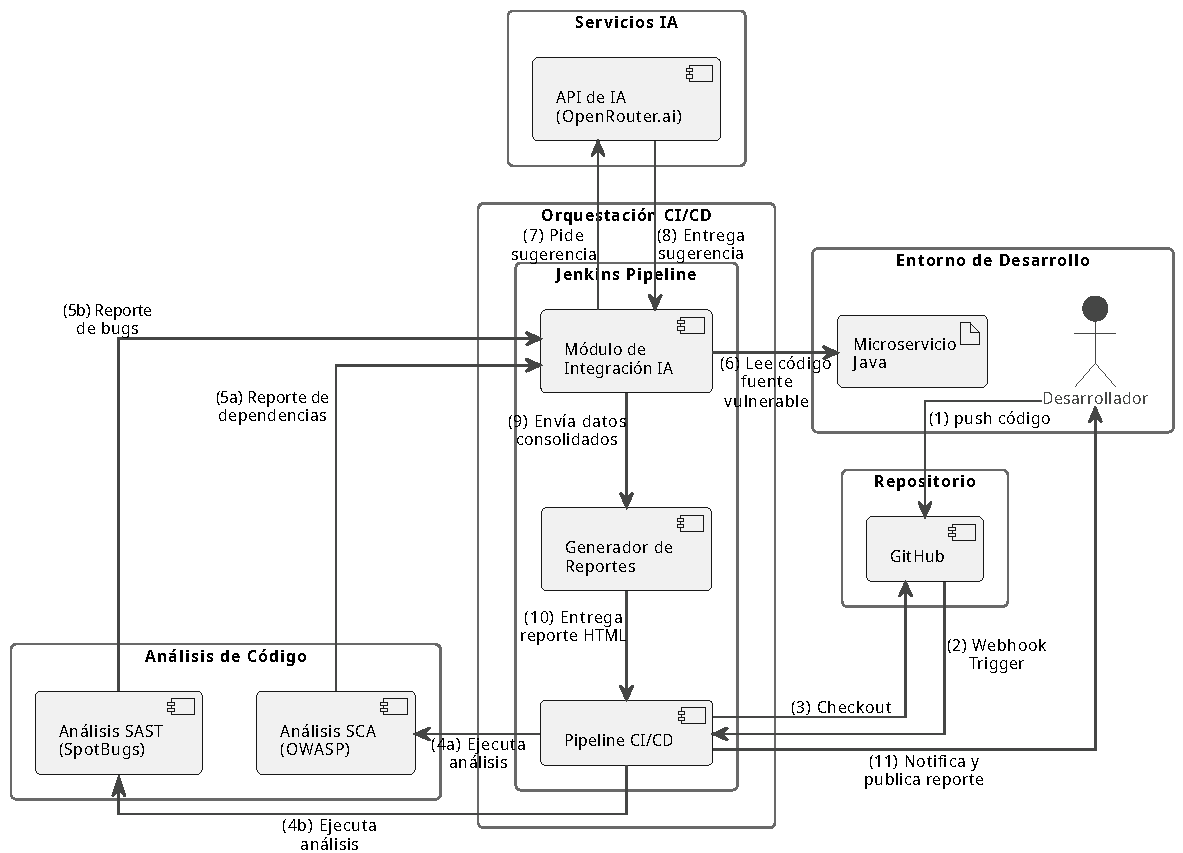
\includegraphics[width=0.9\textwidth]{contenido/imagenes/4_componentes.pdf}
    \caption{Diagrama de componentes del sistema.}
    \label{fig:componentes}
\end{figure}

Como muestra la Figura \ref{fig:componentes}, el pipeline de Jenkins es el orquestador central que invoca a las herramientas de análisis, se comunica con el módulo de IA y finalmente produce el reporte.

\subsubsection{Diagrama de Secuencia}

Este diagrama muestra la interacción entre los componentes a lo largo del tiempo para un solo ciclo de CI/CD.

\begin{figure}[h!]
\centering
\centering
    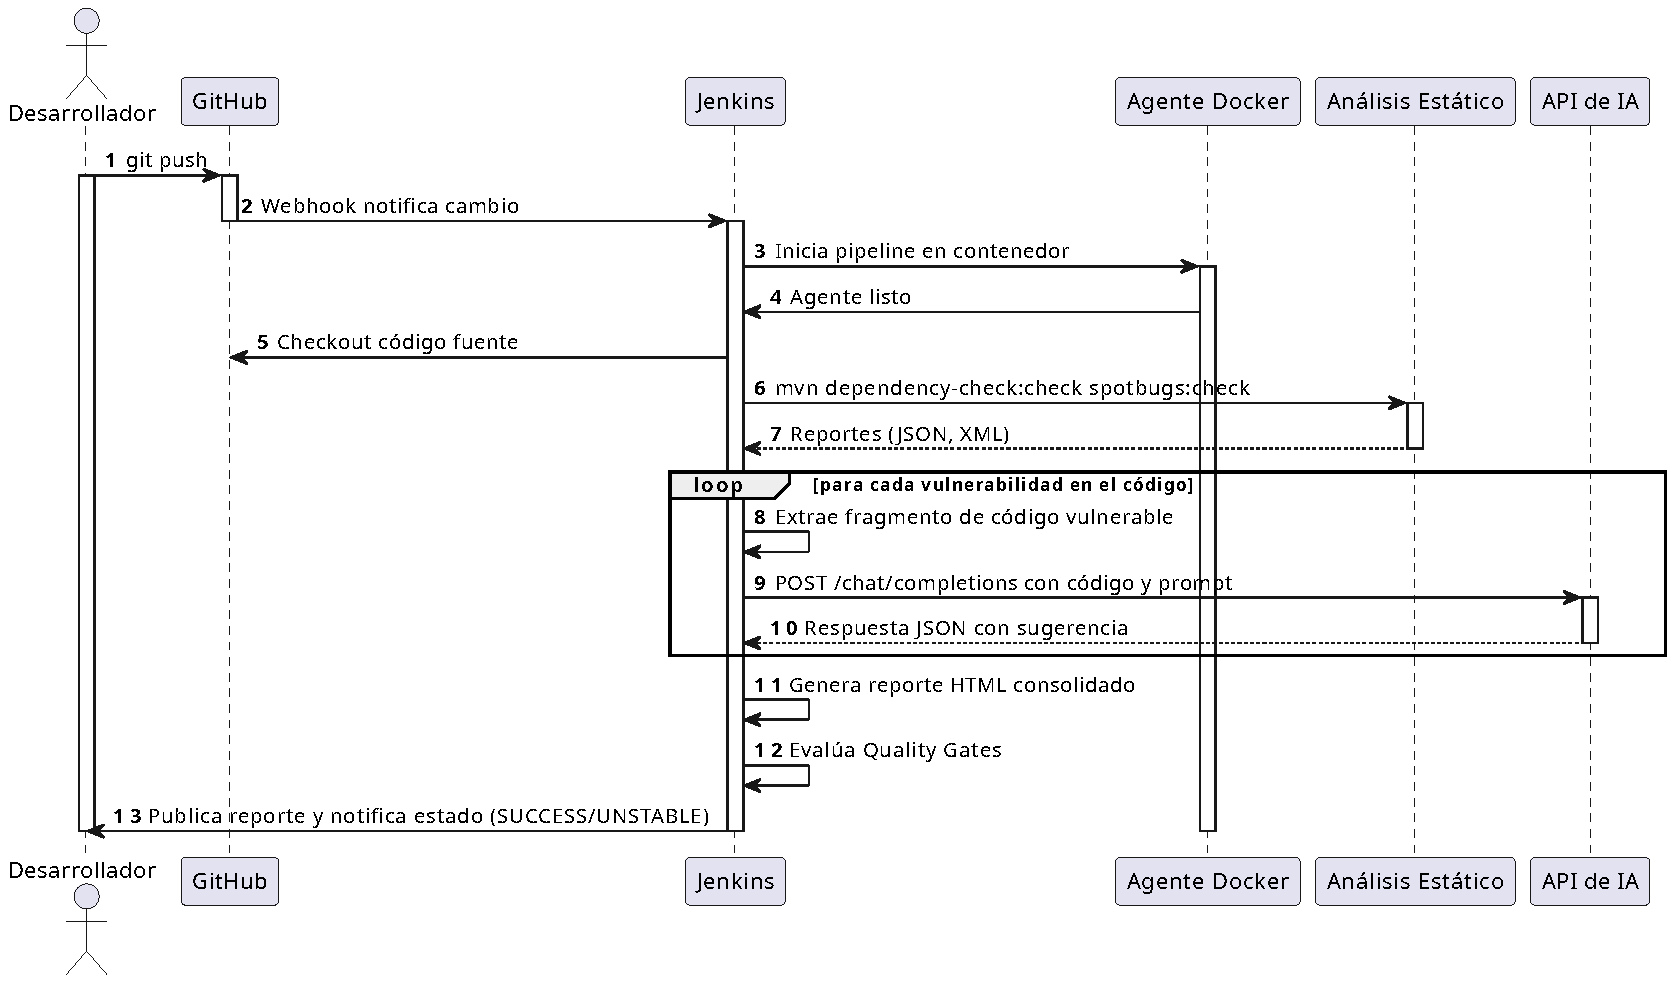
\includegraphics[width=1\textwidth]{contenido/imagenes/4_secuencia.pdf}
    \caption{Diagrama de secuencia del flujo de trabajo DevSecOps.}
    \label{fig:secuencia}
\end{figure}

\subsubsection{Diagrama de Despliegue}

Este diagrama muestra cómo se despliegan físicamente los componentes del software en el hardware.

\begin{figure}[h!]
\centering
\centering
    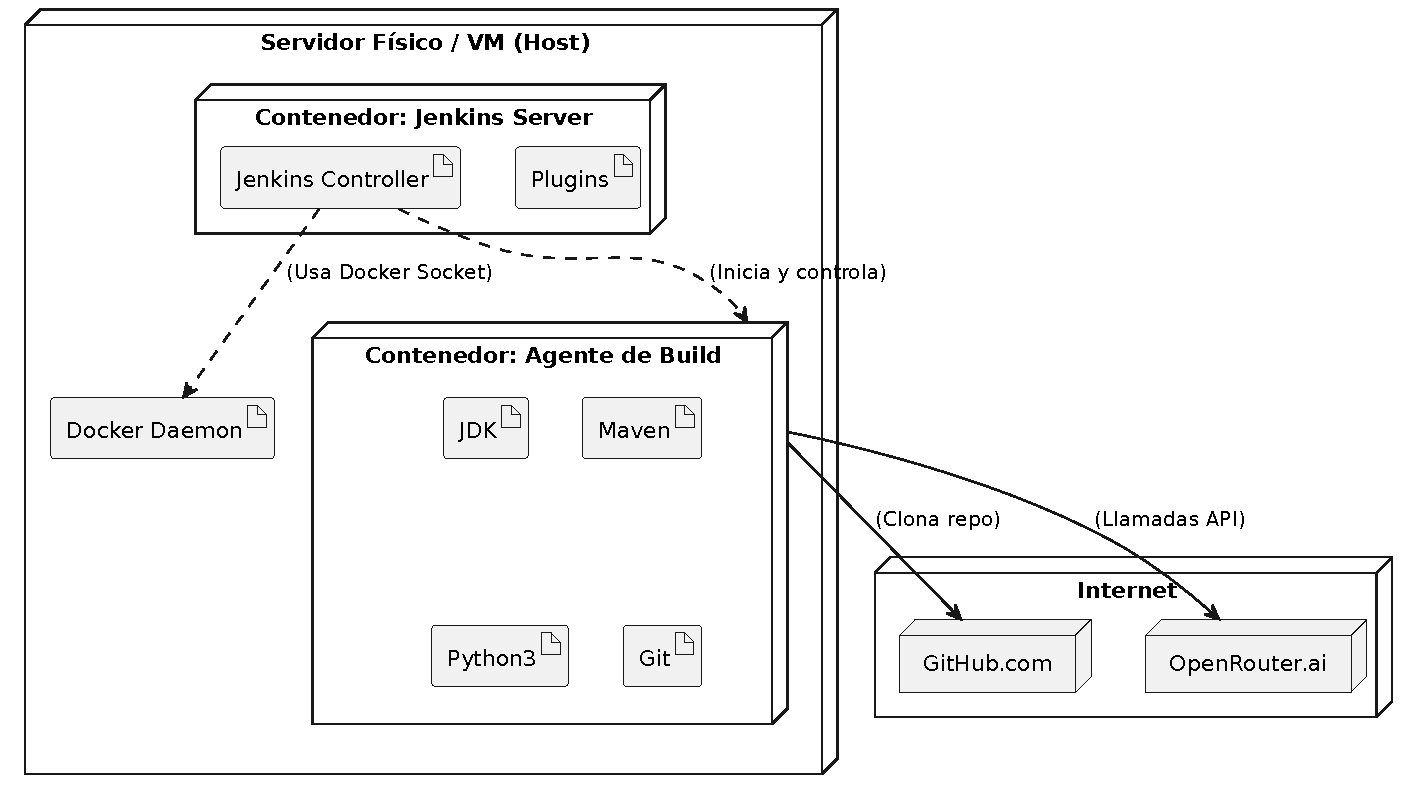
\includegraphics[width=0.8\textwidth]{contenido/imagenes/4_despliegue.pdf}
    \caption{Diagrama de despliegue del entorno.}
    \label{fig:despliegue}
\end{figure}

La Figura \ref{fig:despliegue} ilustra una configuración clave: el contenedor del controlador de Jenkins tiene acceso al Docker socket del host. Esto le permite a Jenkins iniciar otros contenedores, como el `AgentContainer`, donde se realiza todo el trabajo pesado. Esta es una configuración común y flexible conocida como ``Docker-in-Docker''.

A continuación se detalla cada componente de software, archivo de configuración y script de automatización, explicando la implementación práctica y la lógica que gobierna cada decisión de ingeniería.

\subsection{El Entorno de Ejecución Automatizado y Contenerizado}
\label{subsec:entorno_automatizado}

La base de todo el sistema es un entorno de CI/CD consistente, portable y completamente automatizado. Este pilar se construye utilizando Docker para la contenerización y una serie de scripts para la configuración, encarnando los principios de \textbf{Infraestructura como Código (IaC)} y \textbf{Configuración como Código (CasC)}.

\subsubsection{La Plantilla del Entorno: El Dockerfile}
\label{subsubsec:dockerfile_exhaustivo}

El `Dockerfile` actúa como el plano de construcción para la imagen de Docker personalizada sobre la cual se ejecutará Jenkins y todas las tareas del pipeline. Cada instrucción en este archivo fue elegida deliberadamente para construir un entorno autocontenido y completo.

\paragraph{Imagen Base y Privilegios.}
El punto de partida es la imagen oficial `jenkins/jenkins:lts`, que proporciona una versión estable y de soporte a largo plazo de Jenkins. Inmediatamente, se cambia al usuario `root` para obtener los permisos necesarios para instalar paquetes a nivel del sistema operativo.

\paragraph{Instalación de Dependencias del Sistema.}
El comando `apt-get update \&& apt-get install -y ...` instala todas las herramientas que el pipeline necesitará. Cada paquete tiene un rol específico:
\begin{itemize}
    \item \textbf{Herramientas base:} `ca-certificates` es necesario para validar conexiones SSL/TLS, y `curl` se utiliza para descargar archivos de internet, como la clave GPG de Docker.
    \item \textbf{Entorno de Compilación Java:} `maven` y `openjdk-17-jdk` son indispensables para compilar, probar y empaquetar la aplicación de microservicio escrita en Java y Spring Boot.
    \item \textbf{Entorno de Scripting Python:} `python3` y `python3-pip` son necesarios para ejecutar el script de análisis de IA y para instalar sus librerías externas, como `requests`.
\end{itemize}

\paragraph{Instalación del Cliente de Docker.}
Una de las partes más importantes es la instalación del cliente de Docker (`docker-ce-cli`). El proceso sigue las mejores prácticas de seguridad recomendadas por Docker: primero se descarga y añade la clave GPG oficial del repositorio de Docker, y luego se añade el repositorio a las fuentes de `apt`. Esto asegura que se instale un binario de Docker auténtico y permite futuras actualizaciones. Este cliente es lo que permite al contenedor de Jenkins comunicarse con el motor de Docker del sistema anfitrión.

\paragraph{Configuración como Código (CasC) para Jenkins.}
La última sección del Dockerfile se centra en la configuración automática de Jenkins:
\begin{itemize}
    \item \textbf{Instalación de Plugins:} La línea `RUN jenkins-plugin-cli -f /usr/share/jenkins/ref/plugins.txt` es un mecanismo clave de la Configuración como Código. Le dice a Jenkins que lea el archivo `plugins.txt` e instale, durante la construcción de la imagen, todas las extensiones listadas. Esto elimina por completo la necesidad de instalar plugins manualmente desde la interfaz web, haciendo que la configuración sea 100\% reproducible.
    \item \textbf{Scripts de Inicialización:} Se copian los scripts `.groovy` al directorio `init.groovy.d/`. Jenkins está diseñado para ejecutar cualquier script en este directorio la primera vez que arranca con un directorio `/var/jenkins\_home` vacío. Esto permite una configuración cero-toque\footnote{Proceso automatizado que permite configurar y desplegar dispositivos de forma remota y sin intervención manual del usuario.} del sistema.
\end{itemize}

\subsubsection{Configuración Inicial Cero-Toque: Los Scripts de Groovy}
\label{subsubsec:groovy_exhaustivo}

Estos scripts de Groovy son la clave para la automatización completa de la configuración inicial de Jenkins.

\paragraph{El Script \texttt{security.groovy}.}
Este script se encarga de la configuración de seguridad inicial. Su diseño es idempotente, lo que significa que es seguro ejecutarlo múltiples veces.
\begin{enumerate}
    \item Primero, obtiene la instancia actual de Jenkins con \texttt{Jenkins.get()}.
    \item Luego, comprueba si el usuario `admin` ya existe usando \texttt{instance.getUser(``admin'')}.
    \item Si el usuario no existe, procede a crear una configuración de seguridad. Lee la contraseña desde una variable de entorno (`JENKINS\_ADMIN\_PASSWORD'), crea el usuario `admin` y establece una estrategia de autorización segura y estándar.
    \item Si el usuario ya existe, el script imprime un mensaje y finaliza, sin realizar ningún cambio.
\end{enumerate}

\paragraph{El Script \texttt{create\_pipeline.groovy}.}
Este script automatiza la creación del trabajo o job del pipeline principal. Al igual que el de seguridad, es idempotente.
\begin{enumerate}
    \item Comprueba si ya existe un trabajo con el nombre definido en la variable de entorno `PIPELINE\_NAME`.
    \item Si no existe, crea un nuevo WorkflowJob (un pipeline).
    \item La parte más importante es que configura el trabajo para usar `CpsScmFlowDefinition`. Esto le dice a Jenkins que la definición del pipeline debe ser obtenida de un Jenkinsfile ubicado en un repositorio de Git.
    \item Todos los detalles como la URL del repositorio, la rama, la ruta al Jenkinsfile se leen de variables de entorno, haciendo que la creación del pipeline sea totalmente configurable desde el exterior.
    \item Finalmente, ejecuta `instance.reload()` para forzar a Jenkins a recargar su configuración desde el disco, asegurando que el nuevo pipeline sea visible inmediatamente.
\end{enumerate}

\subsection{Orquestación del Servicio: El Archivo \texttt{docker-compose.yml}}
\label{subsubsec:compose_exhaustivo}

Para hacer realidad la arquitectura de despliegue, se utilizó un único archivo `docker-compose.yml`. Este archivo es la receta para construir todo el entorno de CI/CD localmente. Orquesta el servicio de Jenkins con varias directivas clave:
\begin{itemize}
    \item \textbf{restart: always}: Una política de reinicio que asegura la alta disponibilidad del servicio. Si el contenedor se detiene por un error o un reinicio del sistema host, Docker lo levantará automáticamente.
    \item \textbf{volumes}: Define cómo se manejan los datos. El montaje del socket de Docker (`/var/run/docker.sock`) habilita la arquitectura \textbf{Docker-out-of-Docker}, mientras que el volumen nombrado `jenkins\_data` asegura que todos los datos de Jenkins se almacenen de forma segura y persistente.
    \item \textbf{environment}: Esta sección carga las variables desde el archivo `.env`. Separar la configuración (como contraseñas o URLs) en un archivo `.env` es una práctica recomendada que permite modificar el comportamiento del sistema sin tocar los archivos de orquestación.
\end{itemize}

Para iniciar todo el entorno, un usuario solo necesita ejecutar `docker-compose up -d --build` en la terminal, en el mismo directorio donde se encuentra este archivo. Docker se encargará de descargar la imagen de Jenkins, crear los volúmenes y lanzar el contenedor.

En el \textbf{Anexo \ref{anexo:dockercompose}}, se referencia al directorio local ./jenkins\_home, el cual es indispensable ya que contiene toda la configuración, trabajos y datos de Jenkins, asegurando su persistencia entre reinicios del contenedor.
\subsection{Implementación Detallada del Pipeline en Jenkinsfile}

El archivo \texttt{Jenkinsfile} es el cerebro de la automatización de esta tesis. Define, a través de la sintaxis declarativa de Jenkins (\textit{Pipeline as Code}), todo el flujo de trabajo de Integración Continua, Análisis de Seguridad y Despliegue Continuo (CI/Sec/CD). Su propósito es orquestar de manera automática todas las herramientas y procesos, desde que el desarrollador sube el código hasta que se genera un reporte de seguridad accionable.

\subsubsection{Estructura y Entorno del Pipeline}

La sección inicial del archivo \texttt{Jenkinsfile} es fundamental, ya que configura las dos directivas principales que controlan todo el flujo de trabajo: el \textbf{agente de ejecución} y las \textbf{variables de entorno globales}. Estas definiciones establecen dónde se ejecutará el pipeline y qué datos estarán disponibles de manera consistente para todas sus etapas.

\paragraph{Agente de Ejecución.} La primera línea, \texttt{agent any}, es una instrucción crucial. Le dice a Jenkins que puede ejecutar este pipeline en cualquier agente de construcción que esté disponible. En el contexto de nuestro sistema, que se ejecuta enteramente dentro de un único contenedor Docker, esto significa que todas las etapas se llevarán a cabo en el propio controlador de Jenkins. Este agente ya está con todas las herramientas necesarias (Java, Maven, Python, Docker CLI) porque las instalamos directamente en el \texttt{Dockerfile}, garantizando un entorno consistente y rápido.

\paragraph{Variables de Entorno.} El bloque \texttt{environment} se utiliza para declarar variables que estarán disponibles globalmente en todas las etapas. Esto es útil para definir constantes que se usan en múltiples lugares, evitando la repetición y facilitando futuras modificaciones. Las variables clave definidas son:
\begin{itemize}
    \item \texttt{SCAN\_RESULTS\_DIR}: Define un nombre de directorio estándar (`scan-results`) donde todas las herramientas de análisis guardarán sus reportes. Esto crea una ruta consistente para que las etapas posteriores puedan encontrar y procesar los artefactos generados.
    \item \texttt{JAVA\_ANALYSIS\_DIR} y \texttt{MAX\_FILES\_TO\_ANALYZE}: Parametrizan el comportamiento del script de IA, permitiendo ajustar fácilmente el alcance del análisis.
    \item \texttt{AI\_MODEL}: Define qué modelo de IA se utilizará, cumpliendo con el requisito de extensibilidad \textbf{RNF-04}. Cambiar de modelo es tan simple como modificar el valor de esta variable.
\end{itemize}

\subsubsection{Flujo de Trabajo por Etapas (stages)}
El corazón del pipeline se organiza en una secuencia de etapas lógicas, cada una con una responsabilidad clara.

\begin{itemize}
    \item \textbf{Etapa Checkout \& Build}: Esta etapa prepara el entorno y compila la aplicación. El comando \texttt{mvn -Dmaven.test.failure.ignore=true clean package} es deliberado: `clean` asegura que no queden artefactos de compilaciones anteriores, `package` compila y ejecuta las pruebas unitarias, y el parámetro `-Dmaven.test.failure.ignore=true` permite que el pipeline continúe al análisis de seguridad incluso si las pruebas fallan, priorizando la retroalimentación temprana de seguridad.

    \item \textbf{Etapa Unit Test Reports}: Utiliza el paso \texttt{junit} para procesar los reportes XML generados por Maven. Jenkins usa estos datos para mostrar un historial de resultados, visualizar tendencias y permitir un análisis detallado de los fallos.

    \item \textbf{Etapa 'Static Analysis'}: Para optimizar el tiempo (cumpliendo \textbf{RNF-01}), esta etapa utiliza un bloque \texttt{parallel} para ejecutar dos tareas simultáneamente. Mientras una rama ejecuta el análisis SAST con SpotBugs, la otra recopila la lista de archivos Java. El uso de \texttt{try-catch} dentro de la rama de SpotBugs añade resiliencia: un fallo en esta herramienta no detendrá el pipeline, simplemente se registrará.

    \item \textbf{Etapa AI-Powered Analysis}: Es el núcleo innovador del proyecto. Aquí se utiliza el bloque \texttt{withCredentials}, una práctica de seguridad fundamental (cumpliendo \textbf{RNF-03}). Este bloque inyecta la clave de la API de OpenRouter de forma segura como una variable de entorno que solo existe durante la ejecución de este bloque, evitando su exposición en los logs o en el sistema de archivos.

    \item \textbf{Etapa Quality Gate}: Este es el control de seguridad automatizado. Lee el archivo analysis-results.json generado en la etapa anterior y verifica si se cumple la política de seguridad. El uso del paso \texttt{error()} es una decisión de diseño crucial: detiene el pipeline de forma inmediata y lo marca como \texttt{FAILURE} si se encuentra una vulnerabilidad crítica. Esto implementa una política de "cero tolerancia" y previene físicamente que un artefacto inseguro sea desplegado.

    \item \textbf{Etapas Build Docker Image y Local Deploy}: Estas etapas, que solo se ejecutan si el Quality Gate es superado, completan el ciclo de Despliegue Continuo. Demuestran cómo el artefacto validado se empaqueta en una imagen Docker y se despliega, dejando la aplicación funcional para pruebas o su paso a producción.
\end{itemize}

\subsubsection{Acciones Finales y Reportes (post)}
El bloque \texttt{post} es fundamental para la observabilidad y la auditoría del pipeline.
\begin{itemize}
    \item \textbf{always}: Esta condición garantiza que, sin importar si el pipeline tuvo éxito o falló, siempre se intentará publicar los informes (`junit` y `publishHTML`) y archivar los artefactos. Esto es vital, ya que incluso si el pipeline falla, los desarrolladores necesitan acceso a los reportes para entender la causa.
    \item \textbf{success, failure, unstable}: Estos bloques permiten ejecutar acciones contextuales, como enviar notificaciones diferentes a diferentes canales (ej. un email en caso de fallo, un mensaje de Slack en caso de éxito), proporcionando una retroalimentación clara y concisa a los equipos.
\end{itemize}

Para una revisión exhaustiva del código, el contenido completo del \texttt{Jenkinsfile} se encuentra en el \textbf{Anexo \ref{anexo:jenkinsfile}}.

\subsection{El Módulo de Análisis con Inteligencia Artificial}
\label{sec:ai_analyzer_script}
El script de Python \texttt{ai\_code\_analyzer.py} actúa como el motor de análisis que orquesta la interacción entre el código fuente del proyecto y los modelos de lenguaje de gran tamaño (LLMs). Su diseño está orientado a la modularidad, la precisión y la generación de artefactos consumibles tanto por sistemas automatizados como por desarrolladores. El código fuente íntegro de este módulo se adjunta para su consulta en el \textbf{Anexo \ref{anexo:ai_analyzer}}.

\subsubsection{Arquitectura y Funcionamiento General}

El script opera a través de una clase principal, \texttt{OpenRouterAnalyzer}, que encapsula toda la lógica de comunicación y análisis. El flujo de ejecución, orquestado por la función \texttt{main()}, sigue estos pasos:

\begin{enumerate}
    \item \textbf{Inicialización y Configuración:} Al instanciar \texttt{OpenRouterAnalyzer}, el script lee la clave de la API desde la variable de entorno \texttt{OPENROUTER\_API\_KEY} y configura los encabezados HTTP necesarios para la autenticación con el servicio de OpenRouter. Se establece el modelo de IA a utilizar según la jerarquía de prioridades definida.
    \item \textbf{Descubrimiento de Ficheros:} El script escanea el directorio de destino en busca de ficheros \texttt{.java} y \texttt{pom.xml}, que son los objetivos del análisis.
    \item \textbf{Análisis Iterativo:} Para cada fichero identificado, se invoca a la función de análisis correspondiente (\texttt{analyze\_code\_security}, \texttt{analyze\_code\_quality}, o \texttt{analyze\_pom\_security}).
    \item \textbf{Comunicación con la IA:} Cada función de análisis construye un \textit{prompt} específico y lo envía a la API de OpenRouter a través de una llamada POST. El script espera la respuesta del modelo.
    \item \textbf{Procesamiento y Consolidación:} La respuesta de la IA, que se solicita en formato JSON, es parseada y validada. Los resultados de todos los ficheros se consolidan en una única estructura de datos.
    \item \textbf{Generación de Reportes:} Finalmente, con todos los datos consolidados, la función \texttt{generate\_\linebreak report()} crea dos artefactos:
    \begin{itemize}
        \item \textbf{\texttt{analysis-results.json}:} Un fichero JSON estructurado que contiene todos los hallazgos detallados. Su propósito es ser consumido por sistemas automatizados, como el Quality Gate en el pipeline de Jenkins.
        \item \textbf{\texttt{ai-analysis-report.html}:} Un reporte HTML visualmente enriquecido, diseñado para ser fácilmente interpretable por los desarrolladores (Anexo \ref{anexo:ai-analysis-report}).
    \end{itemize}
\end{enumerate}

\subsubsection{Ingeniería de Prompts: La Clave de un Análisis Preciso}

La calidad y precisión del análisis dependen directamente de la calidad de las instrucciones (prompts) enviadas al modelo de IA. Se diseñaron tres prompts distintos, cada uno afinado para una tarea específica. Su estructura se basa en los siguientes principios de la ingeniería de prompts:

\begin{itemize}
    \item \textbf{Asignación de Rol (Role-playing):} Cada prompt comienza con una directiva clara como \textit{``Actúa como un experto en seguridad de aplicaciones Java''}. Esta técnica prepara al modelo, estableciendo el contexto y activando su base de conocimiento relevante para la tarea, lo que resulta en respuestas significativamente más precisas.
    
    \item \textbf{Instrucciones Detalladas y Contextualizadas:} En lugar de una petición genérica, se proporciona una lista numerada de los tipos de vulnerabilidades o problemas de calidad a buscar. Esto funciona como una lista de verificación para el modelo, forzándolo a evaluar el código desde múltiples perspectivas. Además, se incluye el nombre del fichero y el código completo, permitiendo un análisis contextual en lugar de aislado.
    
    \item \textbf{Formato de Salida Estricto:} Se instruye explícitamente al modelo para que responda única y exclusivamente con un objeto JSON válido, proporcionando un ejemplo claro de la estructura deseada. Esta directiva es fundamental para la automatización, ya que garantiza que la salida pueda ser parseada programáticamente por el script sin errores. Para robustecer este proceso, la función \texttt{\_call\_api()} incluye lógica para extraer el bloque JSON de la respuesta, eliminando cualquier texto conversacional que el modelo pudiera añadir.
    
    \item \textbf{Petición de Soluciones Accionables:} Se solicita explícitamente que, de ser posible, se incluya un ejemplo de código corregido (\texttt{code\_correction\_suggested}). Esto va más allá de la simple detección, proveyendo un valor inmenso al desarrollador al ofrecerle una solución tangible y educativa.
\end{itemize}

A continuación, se presentan los prompts exactos utilizados en el script para cada tipo de análisis.

\begin{lstlisting}[language=bash, caption={Prompt para el análisis de seguridad de ficheros Java.}, label={lst:prompt_sec}]
Actúa como un experto en seguridad de aplicaciones Java. Analiza el siguiente código fuente para identificar vulnerabilidades de seguridad:

Archivo: {filename}

Busca específicamente:
1. Inyección SQL
2. Cross-Site Scripting (XSS)
3. Problemas de autenticación/autorización
4. Validación de entrada insuficiente
5. Exposición de información sensible
6. Vulnerabilidades de deserialización
7. Uso inseguro de criptografía
8. Path traversal
9. Command injection
10. Problemas de gestión de sesiones

Código a analizar:
```java
{code_content}
```

Responde en formato JSON con la siguiente estructura:
{{
    "vulnerabilities": [
        {{
            "type": "tipo de vulnerabilidad",
            "severity": "HIGH|MEDIUM|LOW",
            "line": "número de línea aproximado",
            "description": "descripción detallada",
            "recommendation": "cómo solucionarlo",
            "code_correction_suggested": "codigo para solucionar la vulnerabilidad",
            "cwe_id": "CWE-XXX si aplica",
            "impact": "impacto potencial de la vulnerabilidad"
        }}
    ],
    "security_score": "puntuación del 0-10",
    "summary": "resumen ejecutivo de los hallazgos"
}}
\end{lstlisting}

\begin{lstlisting}[language=bash, caption={Prompt para el análisis de calidad de ficheros Java.}, label={lst:prompt_qual}]
Actúa como un experto en calidad de código Java. Analiza el siguiente código para identificar problemas de calidad:

Archivo: {filename}

Evalúa:
1. Code smells y anti-patrones
2. Complejidad ciclomática alta
3. Duplicación de código
4. Problemas de mantenibilidad
5. Violaciones de principios SOLID
6. Uso inadecuado de patrones de diseño
7. Gestión de excepciones
8. Nomenclatura y convenciones
9. Eficiencia y rendimiento
10. Cobertura y calidad de comentarios

Código a analizar:
```java
{code_content}
```

Responde en formato JSON:
{{
    "quality_issues": [
        {{
            "type": "tipo de problema",
            "severity": "HIGH|MEDIUM|LOW",
            "line": "número de línea aproximado",
            "description": "descripción del problema",
            "recommendation": "mejora sugerida",
            "code_correction_suggested": "codigo para solucionar el problema",
            "category": "Maintainability|Reliability|Performance|Documentation",
            "effort": "tiempo estimado para solucionar (minutos)"
        }}
    ],
    "quality_score": "puntuación del 0-10",
    "maintainability_index": "índice de mantenibilidad",
    "complexity_score": "puntuación de complejidad",
    "technical_debt": "deuda técnica estimada en minutos"
}}
\end{lstlisting}

\begin{lstlisting}[language=bash, caption={Prompt para el análisis de seguridad de ficheros POM.}, label={lst:prompt_pom}]
Actúa como un experto en seguridad de proyectos Java Maven. Analiza el siguiente archivo POM para identificar vulnerabilidades de seguridad y problemas de configuración:

Archivo: {filename}

Busca específicamente:
1. Dependencias con vulnerabilidades conocidas (CVE)
2. Versiones desactualizadas de dependencias críticas
3. Dependencias no firmadas o de repositorios inseguros
4. Configuraciones inseguras de plugins
5. Exposición de información sensible en propiedades
6. Configuraciones de Maven que pueden introducir vulnerabilidades
7. Dependencias con scopes inapropiados
8. Plugins sin control de versiones
9. Repositorios HTTP (no HTTPS)
10. Dependencias snapshot en producción

Contenido del POM:
```xml
{pom_content}
```

Responde en formato JSON con la siguiente estructura:
{{
    "vulnerabilities": [
        {{
            "type": "tipo de vulnerabilidad",
            "severity": "HIGH|MEDIUM|LOW",
            "line": "número de línea aproximado o sección",
            "description": "descripción detallada",
            "recommendation": "cómo solucionarlo",
            "code_correction_suggested": "configuración XML para solucionar",
            "cwe_id": "CVE-XXXX si aplica",
            "impact": "impacto potencial de la vulnerabilidad",
            "dependency": "nombre de la dependencia si aplica"
        }}
    ],
    "security_score": "puntuación del 0-10",
    "summary": "resumen ejecutivo de los hallazgos del POM",
    "outdated_dependencies": [
        {{
            "dependency": "nombre de la dependencia",
            "current_version": "versión actual",
            "latest_version": "versión más reciente recomendada",
            "security_risk": "nivel de riesgo de seguridad"
        }}
    ]
}}
\end{lstlisting}

\subsubsection{Uso y Configuración del Script}
El script fue diseñado para ser flexible y fácilmente integrable en flujos de trabajo de CI/CD. Su configuración se gestiona mediante una jerarquía de prioridades que ofrece múltiples formas de invocarlo.

\paragraph{Jerarquía de Prioridades para el Modelo de IA.}
El modelo a utilizar se determina con el siguiente orden de precedencia:
\begin{enumerate}
    \item \textbf{Argumento de línea de comandos:} El uso del flag \texttt{--model} (o \texttt{-mo}) en la terminal tiene la máxima prioridad.
    \item \textbf{Variable de Entorno:} Si no se especifica el argumento, el script buscará la variable de entorno \texttt{AI\_MODEL}.
    \item \textbf{Valor por Defecto:} Si ninguna de las opciones anteriores está presente, se utilizará el modelo predeterminado, codificado en el script como \texttt{google/gemini-2.0-flash-exp:free}.
\end{enumerate}

\paragraph{Argumentos de Línea de Comandos.}
\begin{itemize}
    \item \texttt{--directory}: Especifica el directorio raíz del proyecto a analizar. Si se omite, el script analizará el directorio actual.
    \item \texttt{--model}: Permite definir qué modelo de IA de OpenRouter se debe utilizar para el análisis.
    \item \texttt{--max-files}: Limita el número de ficheros \texttt{.java} a analizar, útil para ejecuciones rápidas o pruebas.
\end{itemize}

\paragraph{Ejemplos de Uso.}
\begin{itemize}
    \item \textbf{Análisis con el modelo por defecto:}
    \begin{verbatim}
    python3 ai_code_analyzer.py --directory /ruta/al/proyecto
    \end{verbatim}
    
    \item \textbf{Especificando un modelo concreto:}
    \begin{verbatim}
    python3 ai_code_analyzer.py --directory /ruta/al/proyecto 
            --model "anthropic/claude-3.5-sonnet"
    \end{verbatim}
    
    \item \textbf{Utilizando una variable de entorno:}
    \begin{verbatim}
    export AI_MODEL="openai/gpt-4o"
    python3 ai_code_analyzer.py --directory /ruta/al/proyecto
    \end{verbatim}
\end{itemize}

\subsection{Desafíos y Soluciones de Implementación}
\label{subsec:desafios_soluciones}
Ningún proyecto de software está exento de problemas. A continuación se detallan los desafíos más significativos encontrados durante el desarrollo y cómo fueron abordados.

\subsubsection{Desafío 1: El Cuello de Botella de los Modelos Locales (Ollama)}

\textbf{Problema:} La intención inicial era utilizar modelos de código abierto como Llama 3 o CodeLlama, ejecutándose localmente en el agente de Jenkins a través de la plataforma Ollama. La ventaja era el coste cero y un mayor control sobre la privacidad de los datos. Sin embargo, las pruebas iniciales revelaron un problema grave de rendimiento. Un modelo de 7 mil millones de parámetros (7B), considerado de tamaño mediano, requería más de 10 GB de RAM y un uso intensivo de CPU. Esto provocaba que la etapa de análisis de un solo archivo tardara varios minutos y, en agentes con recursos limitados, causaba que el sistema se colapsara.

\textbf{Solución:} Se tomó la decisión estratégica de pivotar desde los modelos locales hacia un servicio de API gestionado. Se eligió OpenRouter.ai por su flexibilidad. Este cambio, aunque introducía una dependencia externa y un pequeño coste por uso, resolvió el problema de rendimiento de raíz. La carga computacional se trasladó de la infraestructura local de CI/CD a los servidores optimizados de los proveedores de IA, reduciendo la latencia de minutos a segundos y haciendo que el pipeline fuera viable.

\subsubsection{Desafío 2: Garantizar la Consistencia de la Salida de la IA}

\textbf{Problema:} A pesar de las instrucciones explícitas en el prompt, algunos modelos de IA, especialmente los más pequeños o los que no están afinados para seguir instrucciones (instruction-tuned), a veces fallaban en devolver un JSON perfecto. Podían añadir texto explicativo antes o después del objeto JSON, o incluso generar un JSON con errores de sintaxis (como una coma extra al final de una lista).

\textbf{Solución:} Se implementó una capa de ``limpieza'' en el script de Python. Como se ve en la función `\_call\_ai\_model`, en lugar de asumir que toda la respuesta es JSON, el código busca el primer carácter `{` y el último `}` y extrae el texto intermedio. Esto elimina cualquier texto de relleno. Además, toda la lógica de parseo (`json.loads`) se envolvió en un bloque `try-except` para capturar `JSONDecodeError`. Si el parseo falla, el error se registra y el pipeline continúa, evitando una falla catastrófica por una respuesta malformada de la IA.

\subsubsection{Desafío 3: Gestión Segura de Credenciales}
\textbf{Problema:} El uso de la API de OpenRouter.ai requiere una clave de API, que es un secreto que no debe ser expuesto en el código fuente Jenkinsfile.

\textbf{Solución:} Se utilizó el sistema de gestión de credenciales integrado de Jenkins. Los pasos fueron:
\begin{enumerate}
    \item En la interfaz de Jenkins, ir a `Manage Jenkins -> Credentials`.
    \item Añadir una nueva credencial de tipo ``Secret text''.
    \item Pegar la clave de la API de OpenRouter en el campo ``Secret'' y asignarle un ID, por ejemplo, `openrouter-api-key-id`.
    \item En el `Jenkinsfile`, usar la directiva `credentials()` para inyectar este secreto en una variable de entorno de forma segura, como se muestra en la sección `environment`: `OPENROUTER\_API\_KEY = credentials('openrouter-api-key-id')`.
\end{enumerate}
De esta manera, la clave nunca es visible en el código y está protegida por Jenkins.

\subsubsection{Desafío 4: Consideraciones sobre la Privacidad y Seguridad de los Datos al Usar Servicios de IA de Terceros}
\label{sec:privacidad_datos}

\textbf{Problema:} Al enviar código fuente, potencialmente propietario y sensible, a un servicio de terceros como OpenRouter.ai, surge una preocupación fundamental: ¿cómo se manejan esos datos? Es crucial entender si el código se almacena, si se utiliza para entrenar otros modelos y qué riesgos de seguridad implica para una empresa.

\textbf{Análisis y Solución:} Una investigación de los términos de servicio y la política de privacidad de OpenRouter.ai \cite{OpenRouterTOS} revela varios puntos clave:
\begin{itemize}
    \item \textbf{No almacenamiento por defecto:} La política de OpenRouter establece que, por defecto, no almacenan el contenido de las peticiones (prompts) ni las respuestas de los modelos. Solo se registran metadatos para la facturación y el monitoreo, como las marcas de tiempo y el número de tokens utilizados.
    \item \textbf{Control sobre el entrenamiento de modelos:} OpenRouter actúa como un intermediario. La decisión de si los datos se utilizan para entrenamiento recae en el proveedor del modelo final (por ejemplo, Google, OpenAI, etc.). Sin embargo, OpenRouter proporciona un control granular al usuario. En la configuración de la cuenta, se puede desactivar explícitamente la opción de enviar datos a proveedores que los utilizan para entrenamiento. Si esta opción está desactivada, OpenRouter garantiza que las peticiones solo se enrutarán a modelos y proveedores que se han comprometido a no entrenar con los datos del usuario \cite{OpenRouterPrivacy}.
    \item \textbf{Riesgos residuales:} A pesar de estos controles, el principal riesgo para una empresa reside en la confianza depositada en la cadena de proveedores. Se debe confiar en que OpenRouter cumplirá con su política de enrutamiento y, a su vez, en que el proveedor final del modelo cumplirá con su política de no-entrenamiento. Para una empresa con código fuente altamente sensible o regulado, la única solución para mitigar completamente este riesgo sería utilizar modelos de IA auto-alojados (on-premise), aunque esto reintroduce el \textit{Desafío 1} relacionado con los altos costes de infraestructura y mantenimiento.
\end{itemize}

\textbf{Conclusión:} Para el propósito de esta tesis y para muchas aplicaciones comerciales, los controles ofrecidos por OpenRouter.ai se consideran una solución pragmática y suficientemente segura. Permiten aprovechar la potencia de los modelos más avanzados mientras se mitiga activamente el riesgo de que el código propietario sea utilizado para entrenamiento. La decisión final dependerá siempre de la política de seguridad y el nivel de riesgo aceptable de cada organización.

\subsection{Resumen de la Implementación y Transición a la Evaluación}
A lo largo de este capítulo, se ha detallado el proceso completo de diseño e implementación del prototipo, desde la concepción inicial basada en requisitos funcionales y no funcionales hasta la construcción final de cada componente. Se ha establecido un entorno de CI/CD robusto y reproducible mediante Docker y Jenkins, configurado a través de Infraestructura como Código. Se ha implementado un pipeline Jenkinsfile que orquesta el flujo de análisis, integrando herramientas SAST y el módulo de análisis con IA. Finalmente, se ha descrito el núcleo de la contribución: el script de Python que, mediante una cuidada ingeniería de prompts, interactúa con modelos de lenguaje avanzados para generar sugerencias de mitigación.

Con el prototipo completamente funcional y los desafíos de implementación resueltos, el sistema está listo para ser sometido a prueba. El siguiente capítulo se centrará en la evaluación empírica de la solución, donde se analizará su efectividad, precisión y rendimiento al enfrentarse a un microservicio con vulnerabilidades conocidas, comparando sus resultados con los de herramientas estándar de la industria.

%%%%%%%%%%%%%%%%%%%%%%%%%%%%%%%%%%%%%%%%%%%%%%%%%%%%%%%%%%%%%%%%%%%%%%%
% FIN DEL CAPÍTULO 4
%%%%%%%%%%%%%%%%%%%%%%%%%%%%%%%%%%%%%%%%%%%%%%%%%%%%%%%%%%%%%%%%%%%%%%%
        %%%%%%%%%%%%%%%%%%%%%%%%%%%%%%%%%%%%%%%%%%%%%%%%%%%%%%%%%%%%
% INICIO DEL CAPÍTULO 5
%%%%%%%%%%%%%%%%%%%%%%%%%%%%%%%%%%%%%%%%%%%%%%%%%%%%%%%%%%%%

\chapter{Evaluación y Resultados}
\label{chap:implementacion}
Este capítulo presenta la evaluación empírica y los resultados obtenidos al aplicar la metodología propuesta en esta tesis. Para validar la eficacia de la inteligencia artificial como herramienta de análisis de seguridad, la evaluación se desarrolla en dos fases principales.


Primero, se lleva a cabo una rigurosa comparativa entre cuatro modelos de IA de última generación y dos herramientas de referencia en la industria, SonarQube y Snyk. Utilizando un microservicio deliberadamente instrumentado con 13 vulnerabilidades comunes, se mide no solo la capacidad de detección de cada herramienta, sino también aspectos cualitativos como la calidad de las sugerencias de corrección y la profundidad del análisis. Además, se realiza un estudio cuantitativo del rendimiento y el coste computacional, factores cruciales para la viabilidad en un entorno de desarrollo real.


En la segunda parte, se exponen los resultados de la implementación práctica del modelo de IA más equilibrado en un pipeline de Integración y Despliegue Continuo (CI/CD) completamente automatizado. Se demuestra el ciclo completo de detección, bloqueo de código inseguro mediante un \textit{Quality Gate}, facilitación de la remediación a través de reportes accionables y, finalmente, la validación de las correcciones con una ejecución exitosa del pipeline.

\section{Evaluación}
\label{sec:evaluacion}
Para evaluar la eficacia de la integración de la inteligencia artificial en la detección de vulnerabilidades y mejora de la calidad del código, se ha utilizado un microservicio de ejemplo en Java (alojado en el repositorio \url{https://github.com/iJonnathan/TFM/tree/main/demo}), diseñado a propósito con múltiples fallos de seguridad. Este código fue analizado tanto por los modelos de IA como por dos herramientas de referencia que representan el estándar industrial: SonarQube y Snyk.

\subsection{Entorno de Pruebas y Análisis de Vulnerabilidades}

El componente central para la evaluación es el controlador \texttt{WelcomeController.java} y el fichero \texttt{pom.xml} del proyecto, que contienen un conjunto de vulnerabilidades clásicas para medir la capacidad de detección de las herramientas.

\subsubsection{Análisis Detallado de Vulnerabilidades Introducidas}

Para realizar una evaluación controlada, el microservicio de prueba fue deliberadamente instrumentado con un conjunto de vulnerabilidades, representativas de las categorías más comunes del OWASP Top 10. A continuación, se detalla cada una de ellas:

\textbf{1. Clave Secreta Embebida en el Código (CWE-798):} Se han incluido credenciales directamente en el código fuente.
\begin{lstlisting}[language=java, caption={Claves secretas hardcodeadas.}]
// Hardcoded secret (clave embebida)
private static final String DB_PASSWORD = "SuperSecreta123!";
private static final String API_KEY = "ABC123-TOKEN-INSEGURO";
\end{lstlisting}

\textbf{2. Cross-Site Scripting (XSS) Reflejado (CWE-79):} El endpoint \texttt{/api/welcome} concatena un parámetro en la respuesta sin saneamiento.
\begin{lstlisting}[language=java, caption={Código vulnerable a XSS.}]
@GetMapping("/api/welcome")
public WelcomeDTO welcome( @RequestParam(value = "name", defaultValue = "...") String name) {
    return new WelcomeDTO("Hola, bienvenido " + name + ", esto es un demo");
}
\end{lstlisting}

\textbf{3. Ejecución Remota de Código (RCE) (CWE-94):} El endpoint \texttt{/api/execute} evalúa una cadena del usuario como código, permitiendo la ejecución de comandos arbitrarios.
\begin{lstlisting}[language=java, caption={Código vulnerable a RCE.}]
@PostMapping("/api/execute")
public String executeCode( @RequestBody String userScript) throws Exception {
    ScriptEngine engine = new ScriptEngineManager().getEngineByName("nashorn");
    return "Resultado: " + engine.eval(userScript);
}
\end{lstlisting}

\textbf{4. Path Traversal (CWE-22):} El endpoint \texttt{/api/read-file} permite leer archivos del sistema sin una validación de ruta adecuada.
\begin{lstlisting}[language=java, caption={Código vulnerable a Path Traversal.}]
@GetMapping("/api/read-file")
public String readFile( @RequestParam String filePath) throws Exception {
    return Files.readString(Paths.get(filePath));
}
\end{lstlisting}

\textbf{5. Inyección SQL (CWE-89):} El endpoint \texttt{/api/user} construye una consulta SQL concatenando directamente la entrada del usuario.
\begin{lstlisting}[language=java, caption={Código vulnerable a Inyección SQL.}]
@GetMapping("/api/user")
public String getUserInfo( @RequestParam String username) throws Exception {
    Connection conn = DriverManager.getConnection("jdbc:mysql://localhost:3306/demo", "root", DB_PASSWORD);
    Statement stmt = conn.createStatement();
    ResultSet rs = stmt.executeQuery("SELECT * FROM users WHERE username = '" + username + "'");
    // ...
}
\end{lstlisting}

\textbf{6. Inyección de Comandos (CWE-78):} El endpoint \texttt{/api/ping} ejecuta un comando del sistema operativo concatenando la entrada del usuario.
\begin{lstlisting}[language=java, caption={Código vulnerable a Inyección de Comandos.}]
@PostMapping("/api/ping")
public String ping( @RequestBody String host) throws Exception {
    Process p = Runtime.getRuntime().exec("ping -c 1 " + host);
    // ...
}
\end{lstlisting}

\textbf{7. Deserialización Insegura (CWE-502):} El endpoint \texttt{/api/deserialize} deserializa un objeto de una fuente no confiable sin validación.
\begin{lstlisting}[language=java, caption={Código vulnerable a Deserialización Insegura.}]
@PostMapping("/api/deserialize")
public String deserialize( @RequestBody String base64) throws Exception {
    byte[] data = Base64.getDecoder().decode(base64);
    ObjectInputStream ois = new ObjectInputStream(new ByteArrayInputStream(data));
    Object obj = ois.readObject();
    return "Objeto: " + obj;
}
\end{lstlisting}

\textbf{8. Inserción de Información Sensible en Logs (CWE-532):} El endpoint \texttt{/api/login} registra credenciales en texto plano.
\begin{lstlisting}[language=java, caption={Logs con información sensible.}]
@PostMapping("/api/login")
public String login( @RequestParam String user, @RequestParam String password) {
    logger.info("Intento de login con usuario: " + user + " y contraseña: " + password); // Log inseguro
    return "Login procesado";
}
\end{lstlisting}

\textbf{9. Uso de Criptografía Débil (CWE-327):} El endpoint \texttt{/api/hash} utiliza el algoritmo MD5, que está criptográficamente roto.
\begin{lstlisting}[language=java, caption={Uso de un algoritmo de hash débil (MD5).}]
@GetMapping("/api/hash")
public String hash( @RequestParam String data) throws Exception {
    MessageDigest md = MessageDigest.getInstance("MD5"); // Inseguro
    byte[] digest = md.digest(data.getBytes());
    return Base64.getEncoder().encodeToString(digest);
}
\end{lstlisting}

\textbf{10. Cifrado Simétrico Débil (CWE-326):} El endpoint \texttt{/api/encrypt} usa AES con una clave estática y sin un modo de operación seguro (como GCM).
\begin{lstlisting}[language=java, caption={Cifrado simétrico débil (AES con clave fija).}]
@GetMapping("/api/encrypt")
public String encrypt( @RequestParam String text) throws Exception {
    String key = "1234567890123456"; // Clave estática
    SecretKeySpec secretKey = new SecretKeySpec(key.getBytes(), "AES");
    Cipher cipher = Cipher.getInstance("AES"); // sin GCM ni IV
    cipher.init(Cipher.ENCRYPT_MODE, secretKey);
    return Base64.getEncoder().encodeToString(cipher.doFinal(text.getBytes()));
}
\end{lstlisting}

\textbf{11. Exposición de Información Sensible por Error (CWE-209):} El endpoint \texttt{/api/error} devuelve detalles de la excepción al usuario.
\begin{lstlisting}[language=java, caption={Manejo de excepciones que expone información.}]
@GetMapping("/api/error")
public String error() {
    try {
        int a = 1 / 0;
        return "OK";
    } catch (Exception e) {
        return e.toString(); // Devuelve detalles internos
    }
}
\end{lstlisting}

\textbf{12. Dependencia Vulnerable (CWE-1104):} Se incluyó una versión antigua de la librería `jackson-databind` en el `pom.xml`, conocida por tener vulnerabilidades de deserialización.
\begin{lstlisting}[language=xml, caption={Dependencia vulnerable en pom.xml.}]
<dependency>
    <groupId>com.fasterxml.jackson.core</groupId>
    <artifactId>jackson-databind</artifactId>
    <version>2.9.8</version> 
</dependency>
\end{lstlisting}

\subsection{Modelos y Herramientas de Análisis}

Para llevar a cabo una evaluación exhaustiva y comparativa, se seleccionó un conjunto de modelos de IA de vanguardia y dos herramientas de referencia líderes en la industria.

Los modelos de IA, todos accesibles a través de la plataforma OpenRouter, fueron:
\begin{itemize}
    \item \textbf{google/gemini-2.0-flash-exp:free}: Un modelo de última generación de Google, conocido por su velocidad y capacidades multimodales.
    \item \textbf{deepseek/deepseek-chat:free}: Un modelo de DeepSeek AI especializado y afinado para tareas de conversación y codificación.
    \item \textbf{deepseek/deepseek-r1-0528:free}: Un modelo de código abierto de DeepSeek de alto rendimiento.
    \item \textbf{qwen/qwen-2.5-coder-32b-instruct:free}: Un modelo de Qwen (Alibaba) especializado en código.
\end{itemize}

\paragraph{Herramientas de Referencia (Baselines).}
\begin{itemize}
\item \textbf{SonarQube Community Edition 9.9}: Representa la línea base para el Análisis Estático de Seguridad de
Aplicaciones (SAST) y la calidad del código. Es una de las herramientas más utilizadas en la industria para el análisis del código fuente propio.
\item \textbf{Snyk Open Source}: Representa la línea base para el Análisis de Composición de Software (SCA). Se utilizó la funcionalidad disponible en su plan gratuito, que se enfoca en detectar vulnerabilidades en dependencias de terceros. Es pertinente mencionar que Snyk también ofrece una solución SAST comercial (\textit{Snyk Code}), pero sus capacidades completas forman parte de sus planes de pago y no fueron objeto de esta evaluación \cite{snyk_plans}.
\end{itemize}

\subsection{Análisis Comparativo de Resultados}
\label{subsec:analisis_comparativo_resultados}
Cada modelo de IA y las herramientas de referencia analizaron el proyecto. La siguiente tabla detalla la detección de cada vulnerabilidad específica.

\newcommand{\cmark}{{\color{green!80!black}\checkmark}}%
\newcommand{\xmark}{{\color{red!80!black}\ding{55}}}%

\begin{table}[H]
\centering
\caption{Detección Detallada de Vulnerabilidades por Herramienta}
\label{tab:comparativa_detallada}
\resizebox{\textwidth}{!}{%
\begin{tabular}{|l|c|c|c|c|c|c|}
\hline
\textbf{Vulnerabilidad} & \textbf{SonarQube} & \textbf{Snyk (Free)} & \textbf{Gemini 2.0} & \textbf{DS Chat} & \textbf{DS R1} & 
\textbf{Qwen 2.5} \\
\hline
Hardcoded Secret (Password) & \cmark & N/A & \cmark & \cmark & \cmark & \cmark \\
\hline
Hardcoded Secret (API Key) & \cmark & N/A & \cmark & \cmark & \cmark & \cmark \\
\hline
Cross-Site Scripting (XSS) & \xmark & N/A & \cmark & \cmark & \cmark & \cmark \\
\hline
Remote Code Execution (RCE) & \xmark & N/A & \cmark & \cmark & \cmark & \cmark \\
\hline
Path Traversal & \xmark & N/A & \cmark & \cmark & \cmark & \cmark \\
\hline
Inyección SQL (SQLi) & \xmark & N/A & \cmark & \cmark & \cmark & \cmark \\
\hline
Inyección de Comandos & \xmark & N/A & \cmark & \cmark & \cmark & \cmark \\
\hline
Deserialización Insegura & \xmark & N/A & \cmark & \cmark & \cmark & \cmark \\
\hline
Logs con Datos Sensibles & \xmark & N/A & \cmark & \cmark & \cmark & \cmark \\
\hline
Uso de Criptografía Débil (Hash) & \xmark & N/A & \cmark & \cmark & \cmark & \cmark \\
\hline
Cifrado Simétrico Débil & \cmark & N/A & \cmark & \cmark & \cmark & \cmark \\
\hline
Exposición de Error (Stacktrace) & \xmark & N/A & \cmark & \cmark & \cmark & \cmark \\
\hline
Dependencia Vulnerable (pom.xml) & \xmark & \cmark & \cmark & \cmark & \cmark & \cmark \\
\hline
\hline
\textbf{Total Código Fuente (12)} & 3 & N/A & 12 & 12 & 12 & 12 \\
\hline
\textbf{Total Dependencias (1)} & 0 & 1 & 1 & 1 & 1 & 1 \\
\hline
\end{tabular}%
}
\end{table}

\subsubsection{Análisis Cualitativo de las Respuestas de IA}

Como se estableció en la tabla \ref{tab:comparativa_detallada}, todos los modelos de IA demostraron una capacidad de detección del 100\% en el entorno de prueba. Este resultado, aunque impresionante, oculta diferencias cualitativas importantes en las respuestas que son críticas para un entorno de desarrollo real. A continuación, se analizan ejemplos concretos que ilustran estas diferencias.

\paragraph{Profundidad y Seguridad de la Sugerencia de Corrección.}
Un buen indicador de la calidad de un modelo es la robustez de la solución que propone. Se puede observar una diferencia clara en la gestión de la vulnerabilidad de \textbf{Path Traversal (CWE-22)}.


\begin{itemize}
    \item El modelo \textbf{qwen/qwen-2.5-coder-32b-instruct:free} ofreció la siguiente sugerencia:
    \begin{lstlisting}[language=java,caption={Sugerencia de Qwen para Path Traversal.}]
// Sugerencia de corrección:
if (!filePath.startsWith("/safe/directory/")) {
    throw new IllegalArgumentException("Ruta inválida");
}
    \end{lstlisting}
    \textbf{Análisis:} Esta solución es superficial e insegura. Un atacante podría evadirla fácilmente utilizando secuencias de escape como `filePath = ``/safe/directory/../../etc/passwd'' ', ya que la cadena efectivamente comienza con el prefijo permitido, pero luego navega fuera del directorio seguro.

    \item En contraste, los modelos \textbf{google/gemini-2.0-flash-exp:free} y \textbf{deepseek/deepseek-r1-0528:free} proporcionaron una solución mucho más robusta y segura:
    \begin{lstlisting}[language=java,caption={Sugerencia de Gemini/DeepSeek para Path Traversal.}]
// Sugerencia de corrección:
Path safePath = Paths.get("/safe/directory/").resolve(filePath).normalize();
if (!safePath.startsWith(Paths.get("/safe/directory/"))) {
    throw new IllegalArgumentException("Invalid file path");
}
return Files.readString(safePath);
    \end{lstlisting}
    \textbf{Análisis:} Esta implementación es significativamente superior. El método `.normalize()` resuelve las secuencias `..`, eliminando los intentos de evasión. La posterior validación con `.startsWith()` sobre la ruta ya normalizada asegura que el acceso a ficheros se mantenga estrictamente dentro del directorio previsto. Este es un ejemplo claro de cómo, a pesar de que ambos modelos detectaron la vulnerabilidad, solo uno proporcionó una corrección verdaderamente segura y accionable para el desarrollador.
\end{itemize}

\paragraph{Riqueza del Análisis: Más Allá de la Seguridad.}
Otro diferenciador clave es la capacidad de algunos modelos para ofrecer observaciones valiosas sobre la calidad y mantenibilidad del código, incluso en ficheros sin vulnerabilidades de seguridad. El análisis del fichero \texttt{WelcomeDTO.java} (un simple DTO) es un buen ejemplo.

\begin{itemize}
    \item El modelo \textbf{deepseek/deepseek-r1-0528:free} identificó una mejora de fiabilidad importante:
    \begin{quote}
        \textbf{Descripción:} Class does not override equals() and hashCode(). This may cause unexpected behavior when used in collections. \\
        \textbf{Recomendación:} Implement equals() and hashCode() based on the message field.
    \end{quote}
    \textbf{Análisis:} Esta es una sugerencia de alta calidad. No implementar `equals()` y `hashCode()` en DTOs es una causa frecuente de comportamientos anómalos y errores de difícil depuración cuando estos objetos se utilizan en colecciones como `HashMap` o `HashSet`. Este tipo de feedback proactivo ayuda a mejorar la robustez general de la aplicación.

    \item Por su parte, el modelo \textbf{google/gemini-2.0-flash-exp:free} se enfocó en un principio de diseño de software:
    \begin{quote}
        \textbf{Descripción:} The `message` field is mutable due to the presence of a setter method. For simple DTOs, immutability can improve thread safety and predictability. \\
        \textbf{Recomendación:} If the message should not be changed after creation, remove the `setMessage` method and make the `message` field final.
    \end{quote}
    \textbf{Análisis:} Esta también es una recomendación valiosa que apunta a mejorar la mantenibilidad y a prevenir efectos secundarios no deseados, promoviendo un diseño más funcional y seguro en entornos concurrentes.
\end{itemize}

Estos ejemplos demuestran que, si bien la cobertura de detección de vulnerabilidades es una métrica base, la verdadera diferenciación y el valor para un equipo de desarrollo radican en la calidad, profundidad y seguridad de las recomendaciones generadas, así como en la capacidad del modelo para actuar como un revisor de código integral.

\subsubsection{Análisis Cuantitativo de Rendimiento y Coste}

Más allá de la calidad de la detección, la viabilidad de integrar una solución de IA en un pipeline de CI/CD depende críticamente de dos factores cuantitativos: el \textbf{rendimiento} (tiempo de ejecución) y el \textbf{coste} (consumo de tokens). Un análisis lento puede crear cuellos de botella en el ciclo de desarrollo, mientras que un alto consumo de tokens puede hacer que la solución sea económicamente inviable a escala.

\paragraph{La Importancia de los Tokens.} En los modelos de IA comerciales, el coste se factura por el número de \textit{tokens} procesados. Un token es una unidad de texto (aproximadamente 4 caracteres en inglés). El coste total de una llamada a la API se compone de:
\begin{itemize}
    \item \textbf{Tokens de Entrada (Prompt Tokens):} El tamaño del código y las instrucciones enviadas al modelo. En este experimento, los tokens de entrada fueron constantes para todos los modelos, ya que analizaron los mismos ficheros.
    \item \textbf{Tokens de Salida (Completion Tokens):} El tamaño de la respuesta JSON generada por el modelo. Una respuesta más detallada, con descripciones más largas y sugerencias de código más elaboradas, consume más tokens de salida y, por lo tanto, es más costosa.
\end{itemize}

Para evaluar estos factores, se midió el tiempo de ejecución de cada análisis y se utilizó el tamaño en bytes del fichero de resultados JSON como una métrica proxy del consumo de tokens de salida.
\begin{table}[H]
    \centering
    \caption{Comparativa de Rendimiento y Consumo de Tokens}
    \label{tab:rendimiento_coste}
    \begin{tabular}{|l|c|c|l|}
        \hline
        \textbf{Modelo de IA}                   & \textbf{\makecell{Tiempo de \\ Análisis}} & \textbf{\makecell{Tamaño de \\ Respuesta \\ (Proxy de Tokens)}} & \textbf{Análisis} \\
        \hline
        gemini-2.0-flash-exp:free           & 1 min 38 seg                              & 45.6 KB                                                         & Rápido y detallado \\
        \hline
        deepseek-chat:free                  & 8 min 13 seg                              & 24.8 KB                                                         & \makecell[l]{Lento y moderadamente \\ detallado} \\
        \hline
        deepseek-r1-0528:free               & 18 min 49 seg                             & 16.1 KB                                                         & Muy lento y conciso \\
        \hline
        qwen-2.5-coder-32b-instruct:free    & 4 min 54 seg                              & 49.2 KB                                                & \makecell[l]{Velocidad media, \\ respuesta más extensa} \\
        \hline
    \end{tabular}
\end{table}

\paragraph{Discusión de los Resultados.}
La Tabla \ref{tab:rendimiento_coste} revela un interesante equilibrio entre velocidad, coste y verbosidad:
\begin{itemize}
    \item El modelo \textbf{qwen/qwen-2.5-coder-32b-instruct:free} generó la respuesta más detallada (mayor tamaño), lo que implica un mayor coste en tokens, pero lo hizo en un tiempo razonable. Esto sugiere que es un modelo que prioriza la exhaustividad en sus explicaciones.
    \item El modelo \textbf{google/gemini-2.0-flash-exp:free} emerge como el más equilibrado para un entorno de CI/CD. Ofrece una velocidad de ejecución excepcional (casi 5 veces más rápido que el siguiente) y genera una respuesta muy detallada, representando una excelente relación entre eficiencia, coste y calidad de la información.
    \item El modelo \textbf{deepseek/deepseek-r1-0528:free}, a pesar de ser el más lento, fue sorprendentemente el más conciso en su respuesta. Esto indica un estilo de comunicación muy directo, que podría ser preferible en algunos contextos, pero su alto tiempo de ejecución lo hace menos ideal para pipelines de integración continua que requieren retroalimentación rápida.
\end{itemize}

Este análisis cuantitativo es fundamental para la toma de decisiones en un entorno real. Un equipo podría optar por usar un modelo rápido y económico como \texttt{google/gemini-2.0-flash-exp:free} para las revisiones en cada commit, y reservar el uso de un modelo más lento pero potencialmente más exhaustivo en sus explicaciones para los escaneos nocturnos o previos al despliegue.


Del análisis detallado de los resultados, se extraen las siguientes observaciones clave:

\begin{itemize}
    \item \textbf{Rendimiento de las Herramientas de Referencia (Baselines)}: Las herramientas especializadas demostraron ser eficaces en sus respectivos dominios, pero limitadas fuera de ellos.
        \begin{itemize}
            \item \textbf{SonarQube (SAST)}: Detectó 3 de las 12 vulnerabilidades presentes en el código fuente, enfocándose en patrones evidentes como las claves embebidas. Sin embargo, no identificó ninguna vulnerabilidad contextual (SQLi, XSS) ni la dependencia vulnerable en el \texttt{pom.xml}.
            \item \textbf{Snyk (SCA)}: Como se esperaba de una herramienta SCA líder, identificó con éxito la dependencia vulnerable en el el \texttt{pom.xml} (`jackson-databind`), proporcionando un listado exhaustivo de los 58 problemas de seguridad asociados a esa única dependencia. No obstante, su alcance no cubre el análisis del código fuente propio.
        \end{itemize}

    \item \textbf{Rendimiento Holístico de los Modelos de IA}: El hallazgo más significativo es la capacidad de los modelos de IA para realizar un análisis híbrido, cubriendo tanto las responsabilidades de SAST como de SCA con una eficacia del 100\% en el entorno de prueba. Todos los modelos identificaron la totalidad de las 13 vulnerabilidades, demostrando una comprensión contextual del código y una capacidad para analizar las dependencias del proyecto. Esto representa una ventaja fundamental, ya que ofrecen una visión de seguridad unificada que tradicionalmente requeriría la integración de múltiples herramientas especializadas.

    \item \textbf{Nuevos Criterios de Diferenciación}: Dado que todos los modelos de IA alcanzaron la máxima puntuación en detección, la diferenciación entre ellos ya no se basa en la cobertura, sino en otros factores cualitativos y cuantitativos:
        \begin{itemize}
            \item \textbf{Velocidad y Coste}: Como se observó previamente, existe un claro compromiso. Modelos como google/gemini-2.0-flash-exp:free ofrecen resultados casi instantáneos, mientras que otros como deepseek/deepseek-r1-0528:free son más lentos, lo que puede influir en la elección para distintos tipos de pipelines (CI vs. CD).
            \item \textbf{Calidad del Reporte}: Aunque todos detectaron las vulnerabilidades, la calidad y claridad de las descripciones y, sobre todo, de las sugerencias de corrección, varía entre modelos. Este factor cualitativo es crucial para la accionabilidad de los resultados por parte de los desarrolladores.
            \item \textbf{Análisis de Calidad de Código}: Además de la seguridad, modelos como deepseek-r1-0528:free también proporcionaron un análisis más rico sobre la calidad general del código, similar al de SonarQube, aportando un valor añadido.
        \end{itemize}

    \item \textbf{Complementariedad Re-evaluada}: La idea de complementariedad sigue siendo válida, pero con un nuevo matiz. SonarQube es fundamental para aplicar un conjunto de reglas de código de forma rápida y consistente. La IA, por su parte, no solo complementa, sino que asume el rol principal en la detección de vulnerabilidades de seguridad, ofreciendo una cobertura que antes solo era posible con herramientas comerciales muy costosas o revisiones manuales exhaustivas.
\end{itemize}

\subsection{Conclusión de la Evaluación}

La evaluación empírica llevada a cabo en este trabajo permite extraer una conclusión fundamental: la integración de la Inteligencia Artificial en los pipelines de CI/CD para el análisis de seguridad no solo es una propuesta viable, sino que supera de manera significativa la capacidad de las herramientas de análisis estático gratuitas, como SonarQube Community Edition, en la detección de vulnerabilidades de seguridad complejas.

Mientras que SonarQube se mantiene como una herramienta indispensable para gobernar y mantener la calidad, la fiabilidad y la mantenibilidad del código base, los modelos de IA evaluados han demostrado llenar un vacío crítico en la estrategia de DevSecOps. Su capacidad para realizar un análisis semántico y contextual del código les permite identificar riesgos de seguridad de alto impacto que a menudo pasan desapercibidos para los analizadores basados en reglas estáticas.

La elección final de la herramienta o modelo a integrar dependerá de los objetivos específicos y las restricciones del pipeline de cada organización:
\begin{itemize}
    \item \textbf{Para Calidad de Código y Mantenibilidad}: SonarQube Community sigue siendo la herramienta de referencia indiscutible.
    \item \textbf{Para Máxima Precisión y Cobertura en Seguridad}: El modelo deepseek-r1-0528 demostró ser la opción más segura y exhaustiva, ideal para ejecuciones en pipelines de despliegue a producción o en escaneos de seguridad programados y profundos donde la cobertura total es el objetivo principal.
    \item \textbf{Para un Balance Óptimo entre Seguridad y Agilidad en CI/CD}: Los modelos gemini-2.0-flash-exp y deepseek-chat ofrecen un excelente compromiso, detectando la gran mayoría de las vulnerabilidades críticas en un tiempo de ejecución que se adapta bien a un pipeline de desarrollo activo.
\end{itemize}

En definitiva, una estrategia de DevSecOps madura debería considerar un enfoque híbrido, utilizando SonarQube para establecer una base sólida de calidad de código y complementándolo con un modelo de IA para realizar un análisis de seguridad contextual y profundo, automatizando así una defensa en profundidad directamente en el ciclo de vida del desarrollo.

%%%%%%%%%%%%%%%%%%%%%%%%%%%%%%%%%%%%%%%%%%%%%%%%%%%%%%%%%%%%%%%%%%%%%%%
% FIN DEL CAPÍTULO 4
%%%%%%%%%%%%%%%%%%%%%%%%%%%%%%%%%%%%%%%%%%%%%%%%%%%%%%%%%%%%%%%%%%%%%%%
\section{Resultados de la Ejecución del Pipeline}
\label{subsec:analisis_resultados_pipeline}

Para la validación empírica de la solución, se diseñó una prueba específica utilizando el microservicio (`demo`). A diferencia de la comparativa inicial que abarcó trece vulnerabilidades, esta fase se concentró en un subconjunto de \textbf{cinco vulnerabilidades} para evaluar de forma precisa el comportamiento de la solución integrada en el pipeline.

El modelo de IA seleccionado para esta prueba fue \texttt{gemini-2.0-flash-exp}. Esta elección se justifica por su rendimiento superior en la evaluación comparativa (sección \ref{subsec:analisis_comparativo_resultados}), donde demostró el mejor equilibrio entre precisión, calidad de las sugerencias y eficiencia.

Con el entorno CI/CD completamente automatizado, la ejecución del pipeline se activó tras realizar un `commit` en el repositorio, cumpliendo con el requisito \textbf{RF-01}. La vista general del proceso, con las etapas completadas y el punto de fallo, se puede apreciar en la Figura \ref{fig:pipeline_general_fail_alt}.

\begin{figure}[h]
\centering
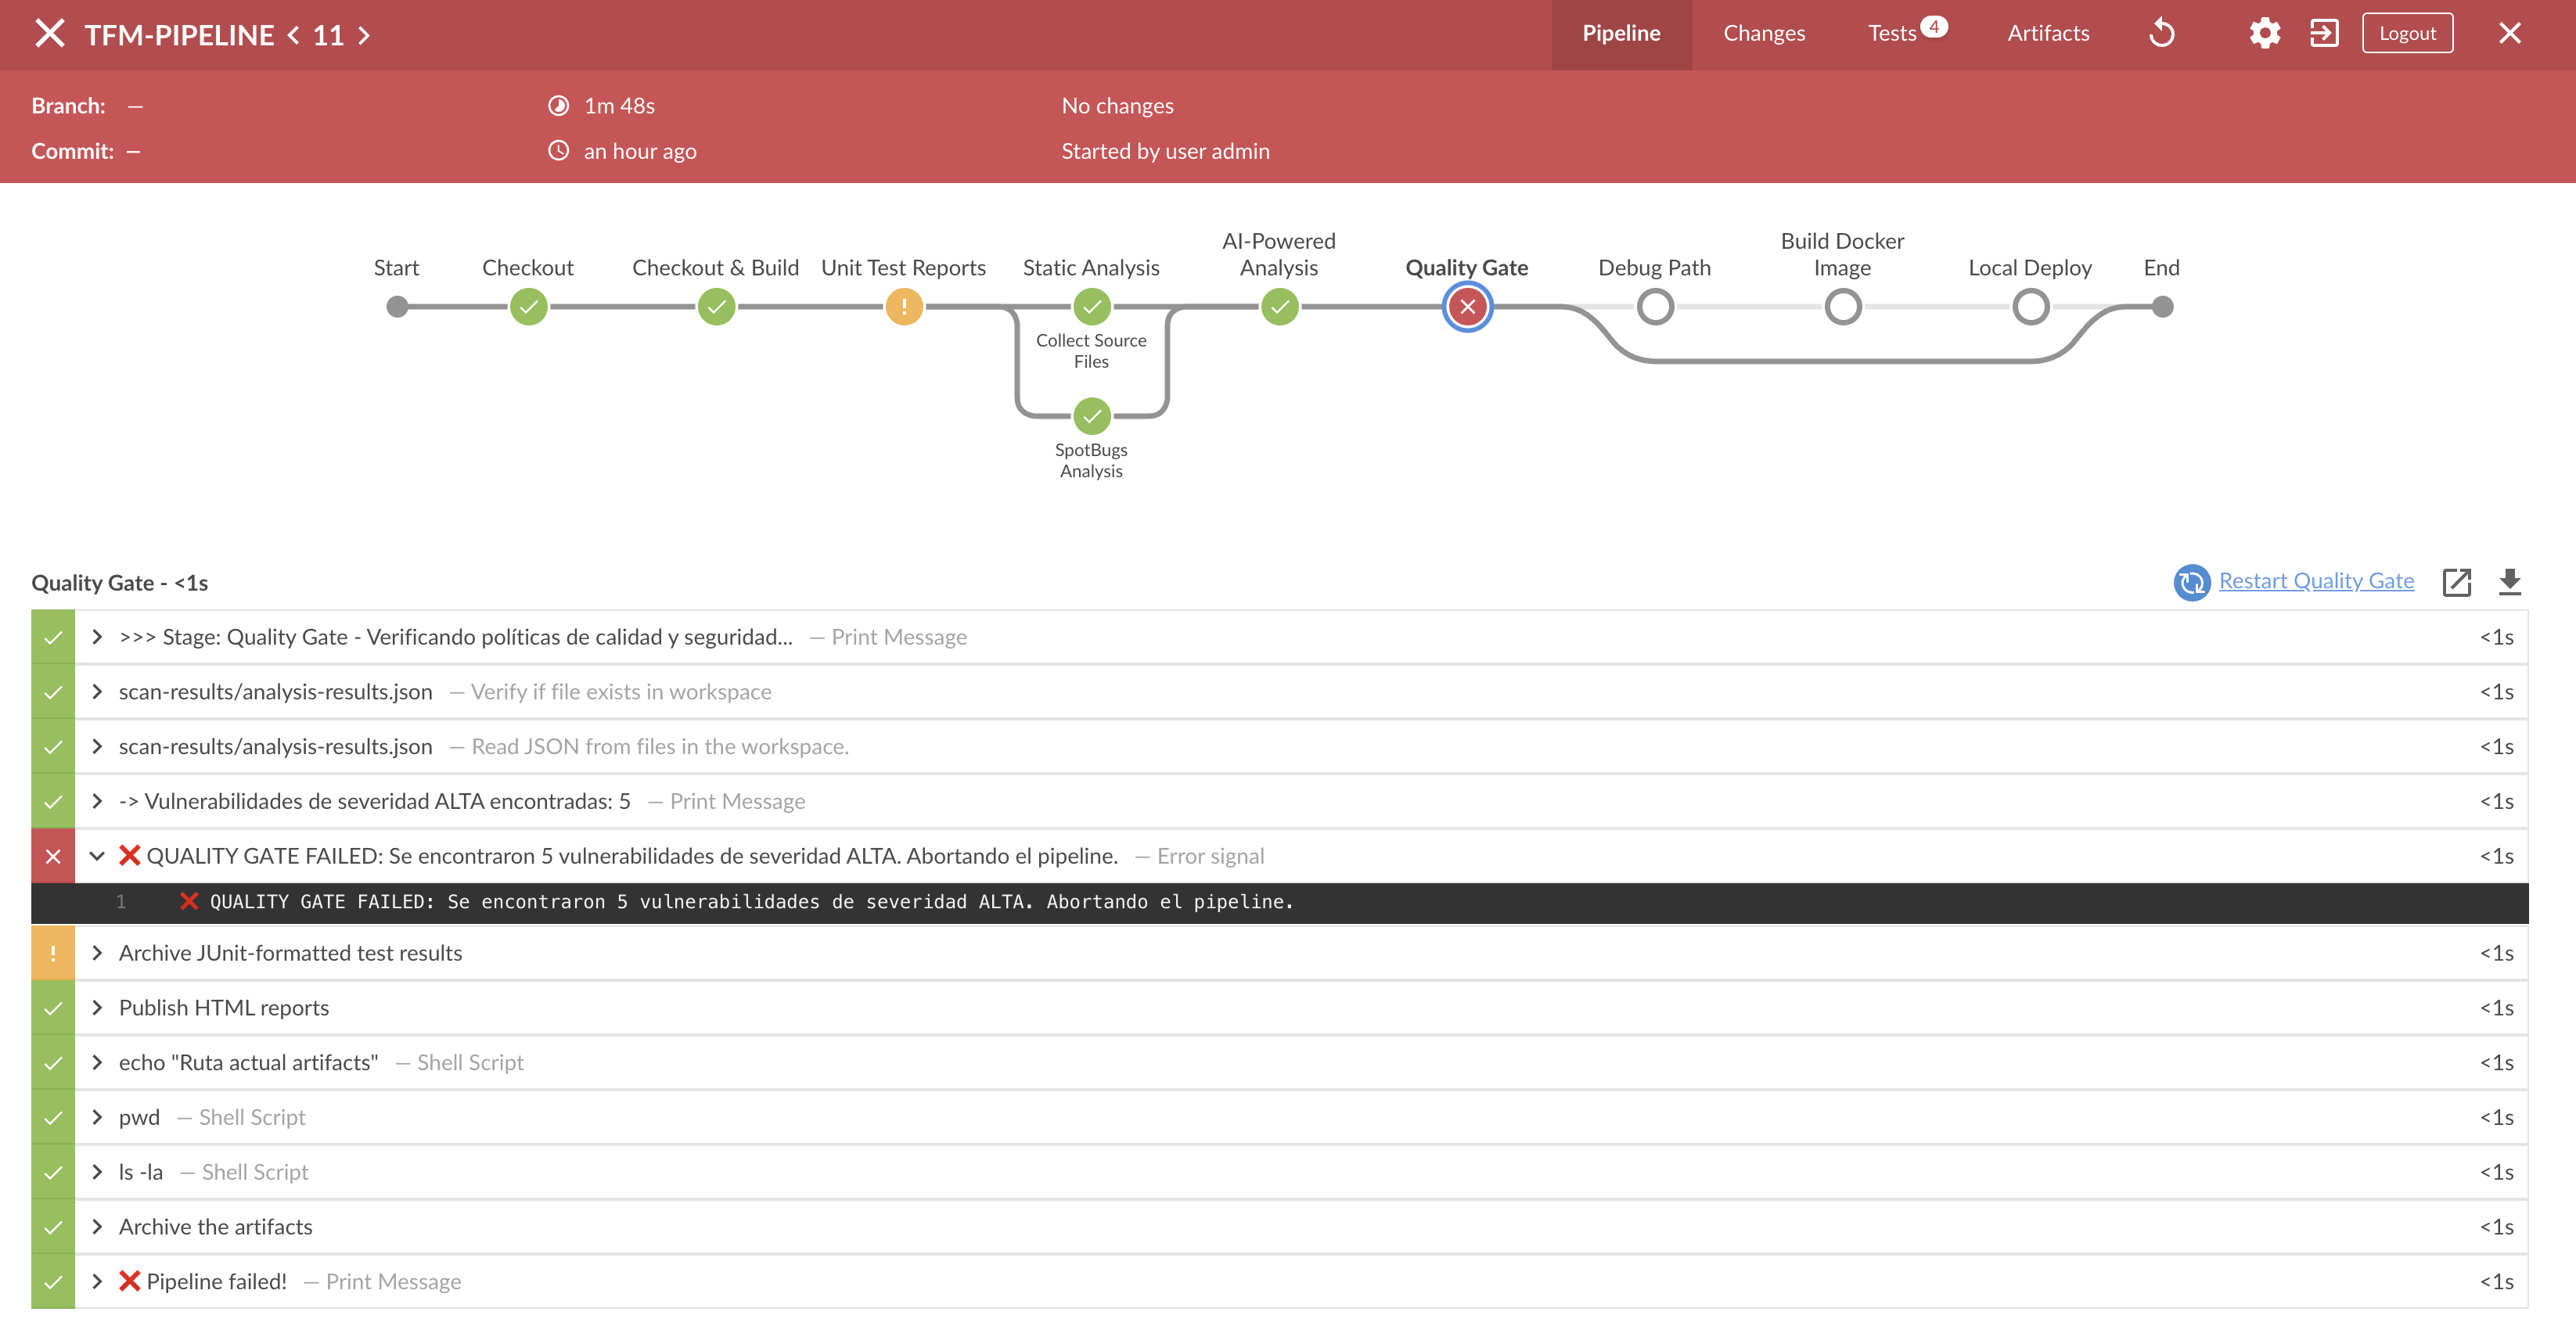
\includegraphics[width=0.99\textwidth]{contenido/imagenes/4_pipeline_fail.png}
\caption{Ejecución fallida del pipeline.}
\label{fig:pipeline_general_fail}
\end{figure}

\subsubsection{Flujo de Ejecución y Falla Controlada en el Quality Gate}
El pipeline ejecutó las primeras etapas de manera secuencial y paralela, tal como fue diseñado, recopilando información de seguridad en cada paso antes de llegar al punto de control crítico.

\begin{enumerate}
    \item Las etapas iniciales, \textbf{Checkout \& Build} y \textbf{Unit Test Reports}, se completaron con éxito. El código fue clonado, la aplicación fue empaquetada con Maven (\textbf{RF-02}), y los reportes de pruebas unitarias fueron procesados por Jenkins, sin embargo, una de las pruebas unitarias saltó una excepción debido a una vulnerabilidad de dependencia en el pom.xml, el cual fue detectada en el stage AI-Powered Analysis.
    \item La etapa \textbf{Static Analysis} se ejecutó, realizando sus tareas en paralelo para optimizar el tiempo.
    \item La etapa \textbf{AI-Powered Analysis} se completó satisfactoriamente, cumpliendo su objetivo principal (\textbf{RF-04}). El script de Python interactuó con la API de la IA y generó los artefactos cruciais: el reporte HTML para el desarrollador (`ai-analysis-report.html`) y el reporte JSON (`analysis-results.json`) para la automatización, cumpliendo así con \textbf{RF-05}.
    \item La ejecución llegó a la etapa \textbf{Quality Gate}. Este es el punto de control automatizado que implementa la política de seguridad del pipeline. El script leyó el archivo analysis-results.json y, tal como se esperaba, encontró que el valor de high\_severity\_vulnerabilities era de 5. 
\end{enumerate}

Debido a que este valor era mayor que el umbral de cero definido en la política, la condición del Quality Gate se activó y ejecutó el paso error(). Este comando detuvo inmediatamente el pipeline y lo marcó con el estado \textbf{FAILURE}, como se evidencia en la captura de la Figura \ref{fig:pipeline_general_fail}. Como resultado, las etapas posteriores Debug Path, Build Docker Image y Local Deploy nunca se ejecutaron.

Este fallo controlado es un éxito rotundo para el experimento. Demuestra que el sistema funciona como un mecanismo de seguridad preventivo eficaz (cumpliendo \textbf{RF-06}), deteniendo físicamente la promoción de código inseguro a través del ciclo de vida de desarrollo.

\subsubsection{Análisis Detallado del Reporte Generado por la IA}
La pieza clave generada por el pipeline es el reporte en formato HTML. Este documento, fácil de leer para los desarrolladores, es la principal herramienta para entender y solucionar los problemas encontrados. El reporte completo de esta ejecución se encuentra en el \textbf{Anexo \ref{anexo:ai-analysis-report}}.

A continuación, se explican los problemas más graves que encontró la IA y que causaron la falla del Quality Gate.

\paragraph{Dependencia Vulnerable en `pom.xml` (Severidad: HIGH)}
\begin{itemize}
    \item \textbf{Hallazgo:} La IA revisó el archivo pom.xml y vio que se usaba la versión 2.9.8 de la librería jackson-databind. Avisó que esta versión es muy antigua y tiene fallos de seguridad graves (CVEs) que podrían permitir a un atacante ejecutar código en el servidor.
    \item \textbf{Sugerencia de la IA:} La solución fue simple y directa: actualizar la librería a una versión más nueva y segura (como 2.16.1 o superior) en el archivo pom.xml.
\end{itemize}

\paragraph{Inyección SQL (Severidad: CRITICAL)}
\begin{itemize}
    \item \textbf{Hallazgo:} En el WelcomeController, la IA detectó que una consulta a la base de datos se estaba construyendo uniendo texto con datos que venían de un usuario, sin ninguna protección. Esto es un riesgo clásico de Inyección SQL.
    \item \textbf{Sugerencia de la IA:} Recomendó usar consultas preparadas (PreparedStatement), que es la forma correcta y segura de hacerlo, e incluyó un ejemplo de código de cómo implementarlo.
\end{itemize}

\paragraph{Ejecución Remota de Código (RCE) (Severidad: CRITICAL)}
\begin{itemize}
    \item \textbf{Hallazgo:} El sistema identificó que una parte del código ScriptEngine.eval() ejecutaba comandos directamente de la entrada del usuario, lo que es un riesgo crítico.
    \item \textbf{Sugerencia de la IA:} La recomendación fue eliminar esa función por completo, lo cual es la decisión más segura cuando una característica es tan peligrosa.
\end{itemize}

\paragraph{Path Traversal (Severidad: HIGH)}
\begin{itemize}
    \item \textbf{Hallazgo:} La IA señaló que una función que leía archivos tomaba la ruta del archivo directamente de la entrada del usuario, lo que le permitiría a un atacante leer archivos prohibidos del sistema usando secuencias como `../`.
    \item \textbf{Sugerencia de la IA:} Sugirió añadir código para verificar que la ruta del archivo solicitado estuviera siempre dentro de una carpeta base segura y permitida.
\end{itemize}

\paragraph{Claves Secretas en el Código (Severidad: CRITICAL)}
\begin{itemize}
    \item \textbf{Hallazgo:} El modelo encontró que la contraseña de la base de datos y una clave de API estaban escritas directamente en el código.
    \item \textbf{Sugerencia de la IA:} Recomendó seguir las mejores prácticas de seguridad (cumpliendo \textbf{RNF-03}) y mover estos secretos a variables de entorno o a un sistema de gestión de credenciales, en lugar de tenerlos en el código.
\end{itemize}
\subsubsection{Remediación y Ejecución Exitosa del Pipeline}
\label{subsec:remediacion_exitosa}

El valor fundamental del prototipo no reside únicamente en la detección, sino en su capacidad para facilitar una remediación rápida y precisa. Con las instrucciones claras y los ejemplos de código proporcionados por el reporte de la IA, un desarrollador pudo proceder a corregir las 5 vulnerabilidades críticas identificadas. El proceso de remediación consistió en:
\begin{itemize}
    \item Actualizar la versión de la dependencia `jackson-databind` en el archivo `pom.xml` a una versión segura.
    \item Refactorizar el método `getUserInfo` en WelcomeController.java para utilizar PreparedStatement, eliminando así la vulnerabilidad de Inyección SQL.
    \item Eliminar por completo los métodos inseguros executeCode (RCE) y ping (Command Injection).
    \item Añadir la lógica de validación de rutas en el método readFile para prevenir el Path Traversal.
    \item Externalizar las claves secretas (`DB\_PASSWORD` y `API\_KEY`), eliminándolas del código fuente y configurándolas como variables de entorno seguras.
\end{itemize}

Una vez aplicados estos cambios y subido el código corregido al repositorio de GitHub, el pipeline de Jenkins se ejecutó por segunda vez.

En esta nueva ejecución, el flujo de trabajo fue notablemente diferente. La etapa de `AI-Powered Analysis` analizó el código corregido y generó un nuevo reporte que no contenía ninguna vulnerabilidad de severidad `HIGH` o `CRITICAL`. Consecuentemente, al llegar a la etapa de `Quality Gate`, el resultado fue positivo. El log de la consola mostró el mensaje esperado: `QUALITY GATE PASSED: No se encontraron vulnerabilidades de severidad ALTA.`.

Al superar con éxito esta puerta de calidad, en primer lugar, la etapa de pruebas unitarias que anteriormente falló, esta vez ejecutó con éxito las 2 pruebas unitarias. El pipeline no se detuvo, continuó su ejecución a través de las etapas restantes:

\begin{enumerate}
    \item La etapa \textbf{Build Docker Image} se ejecutó sin problemas, tomando el archivo `.jar` seguro y empaquetándolo en una imagen Docker llamada `demo-app`.
    \item La etapa final, \textbf{Local Deploy}, también se completó exitosamente. Detuvo y eliminó cualquier versión anterior del contenedor de la aplicación y desplegó la nueva imagen, dejando el microservicio corregido y funcional, tal como se observa en la \textbf{Figura \ref{fig:deploy_exitoso}}.
\end{enumerate}

\begin{figure}[H]
    \centering
    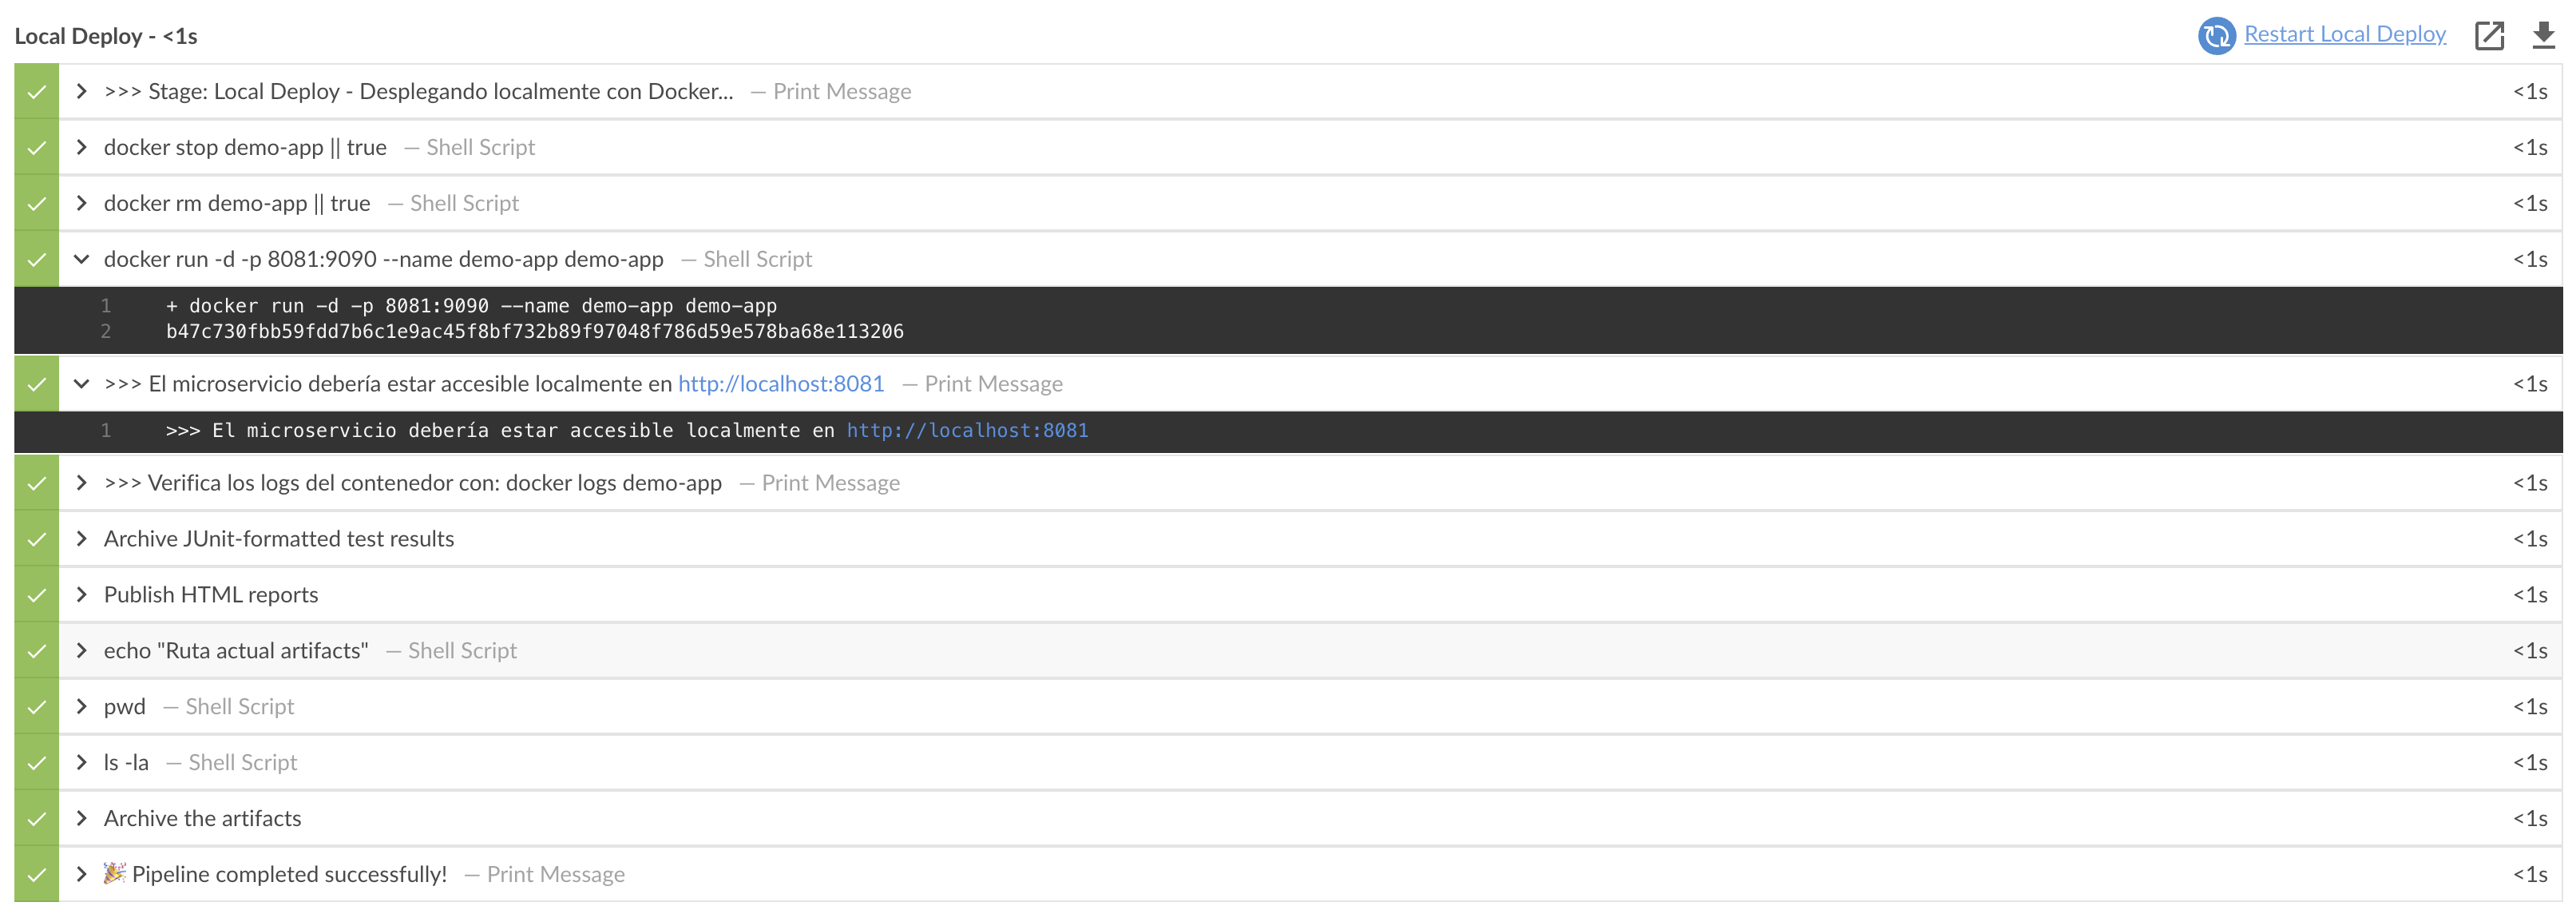
\includegraphics[width=0.9\textwidth]{contenido/imagenes/4_deploy_ok.png}
    \caption{Despliegue exitoso de la etapa de despliegue.}
    \label{fig:deploy_exitoso}
\end{figure}

En conclusión, el ciclo de evaluación demostró ser un éxito completo. La primera ejecución validó la capacidad del sistema para detectar riesgos y actuar como un mecanismo de control preventivo, deteniendo un despliegue inseguro. La segunda ejecución, tras aplicar las correcciones sugeridas por la IA, validó la utilidad y precisión de dichas sugerencias, permitiendo que un artefacto seguro completara el pipeline de principio a fin, como se evidencia en la ejecución final de la \textbf{Figura \ref{fig:pipeline_exitoso}}. Este proceso empírico confirma que la integración de asistencia por IA en un pipeline CI/CD no solo es viable, sino que acelera eficazmente el ciclo de remediación, cumpliendo así con los objetivos centrales de esta tesis.

\begin{figure}[H] 
    \centering
    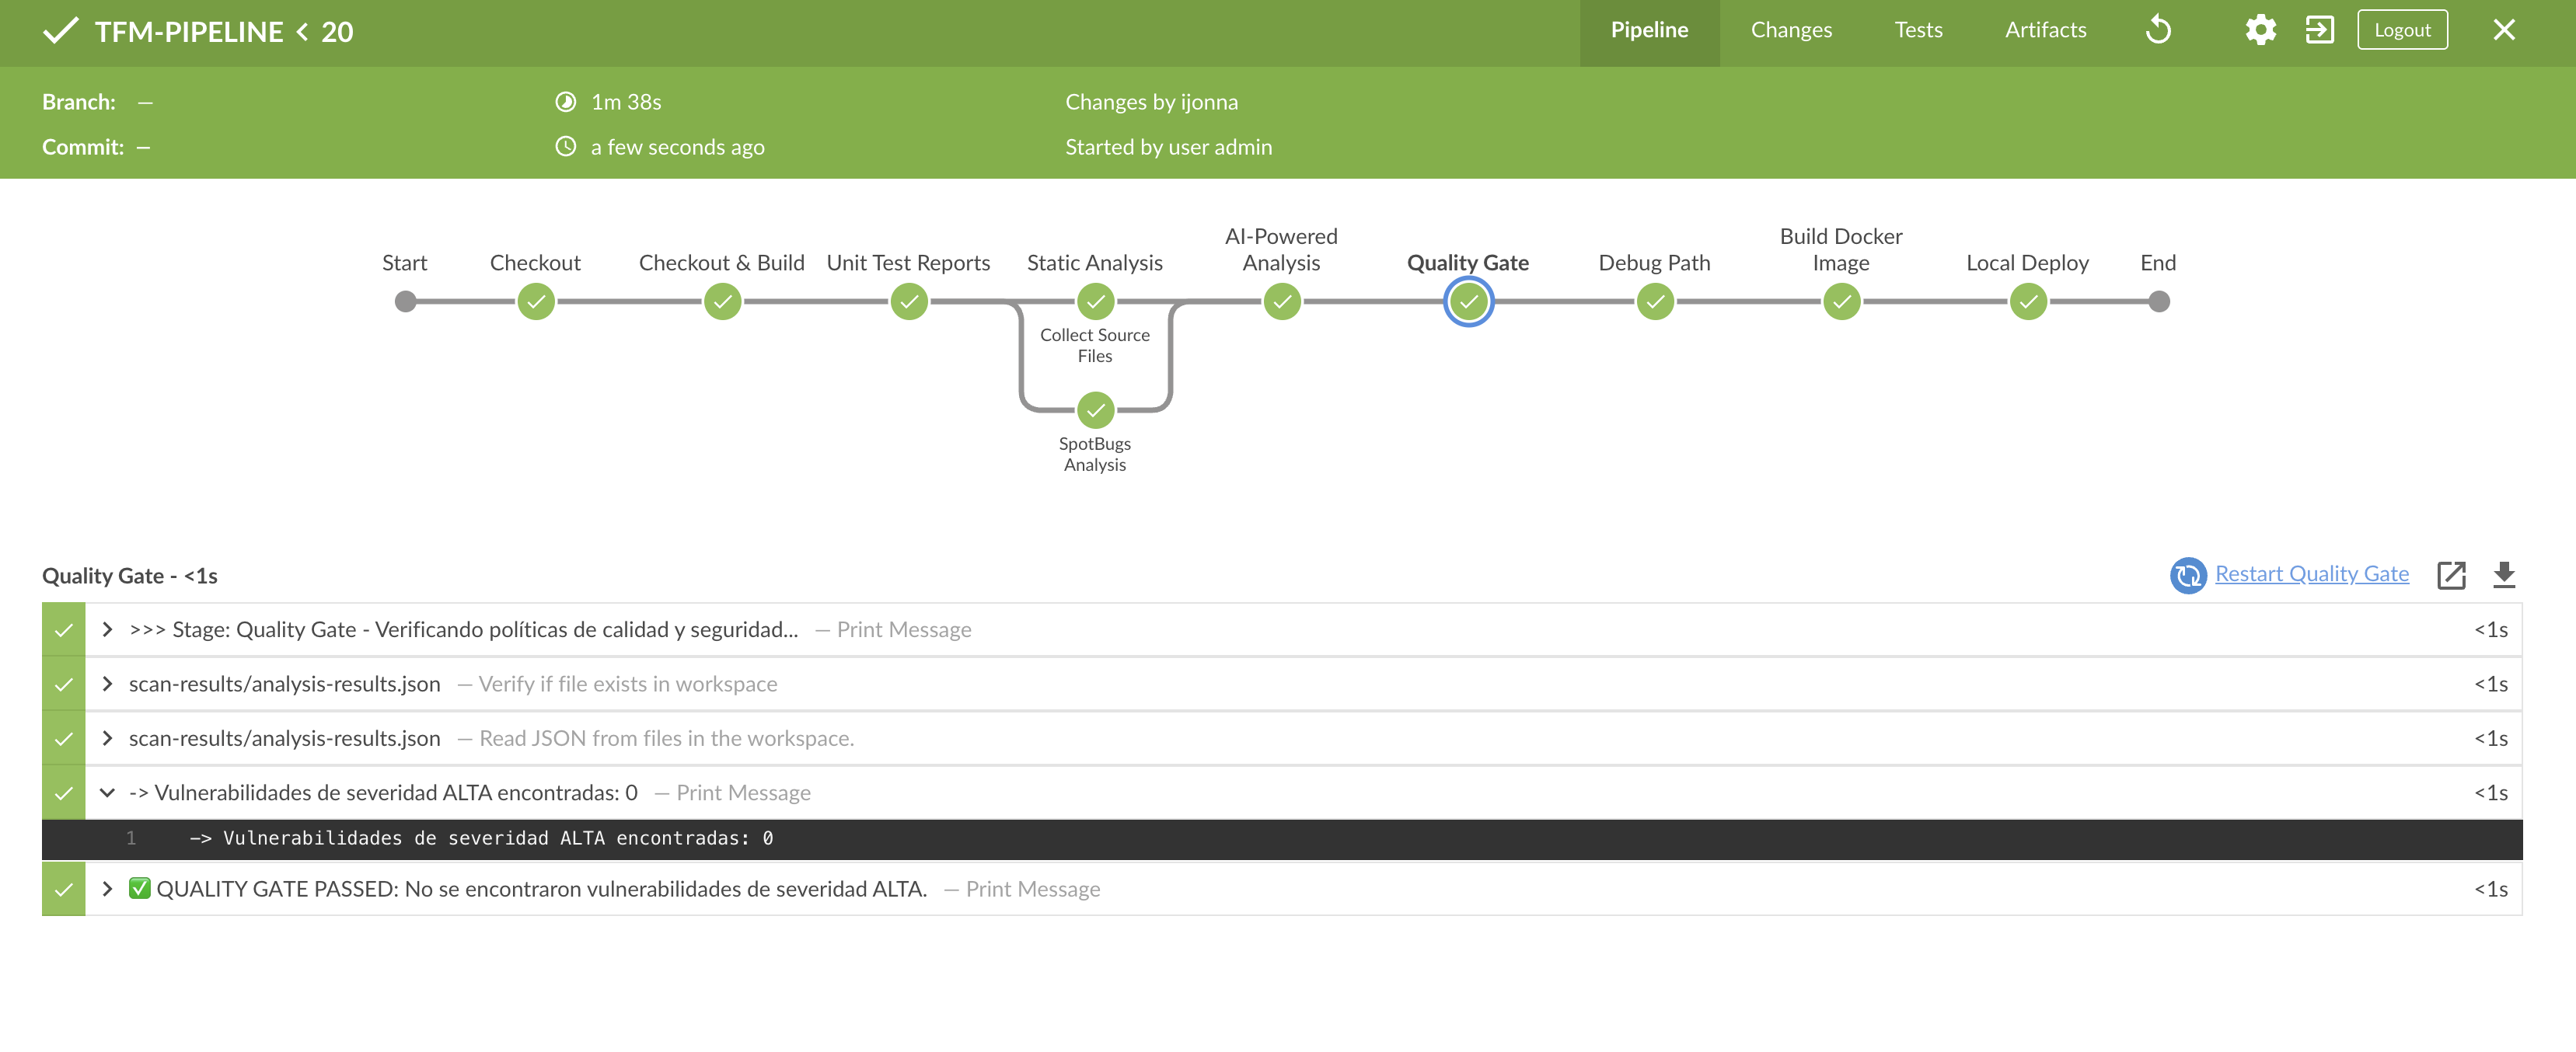
\includegraphics[width=0.9\textwidth]{contenido/imagenes/4_pipeline_ok.png}
    \caption{Ejecución exitosa del pipeline.}
    \label{fig:pipeline_exitoso}
\end{figure}

%%%%%%%%%%%%%%%%%%%%%%%%%%%%%%%%%%%%%%%%%%%%%%%%%%%%%%%%%%%%%%%%%%%%%%%
% FIN DEL CAPÍTULO 5
%%%%%%%%%%%%%%%%%%%%%%%%%%%%%%%%%%%%%%%%%%%%%%%%%%%%%%%%%%%%%%%%%%%%%%%
        \chapter{Conclusiones y Trabajo Futuro}\label{chap:conclusiones_trabajo_futuro}

Este capítulo final sintetiza los hallazgos y contribuciones de la presente investigación, evalúa el grado de cumplimiento de los objetivos propuestos y establece una visión para futuras líneas de desarrollo que pueden expandir y mejorar el trabajo realizado.

\section{Conclusiones}\label{sec:conclusiones}

La proliferación de arquitecturas de microservicios y la consolidación de las prácticas DevOps han impuesto un ritmo de entrega de software sin precedentes. Sin embargo, esta agilidad a menudo introduce un desafío crítico: la gestión eficaz y oportuna de la seguridad. El problema central abordado en esta tesis fue la brecha existente entre la detección de vulnerabilidades y su efectiva mitigación, un proceso que tradicionalmente recae en el desarrollador y que puede ser lento, propenso a errores y carente del contexto necesario.

Para enfrentar este desafío, el \textbf{objetivo general} de este trabajo fue diseñar, implementar y evaluar un prototipo que integrara la Inteligencia Artificial (IA) en pipelines CI/CD para generar sugerencias de mitigación de vulnerabilidades en microservicios Java. Tras un proceso de desarrollo y evaluación riguroso, se puede afirmar que este objetivo se ha cumplido satisfactoriamente.

El prototipo funcional, orquestado en Jenkins y utilizando un `Jenkinsfile` como pilar del \textit{Pipeline as Code}, ha demostrado la viabilidad de la hipótesis central: es posible automatizar no solo la detección, sino también la generación de orientación para la corrección de fallos de seguridad. A continuación, se detallan las conclusiones en relación con los objetivos específicos:

\begin{enumerate}
    \item \textbf{Respuesta a los Objetivos Específicos:} Se logró la integración exitosa de herramientas SAST (`SpotBugs`) y SCA (`OWASP Dependency-Check`) en un pipeline de Jenkins. Se seleccionó y se integró un modelo de IA a través de la plataforma `OpenRouter.ai`, lo que proporcionó flexibilidad para evaluar diferentes LLMs. Se desarrolló la lógica de organización en Python, que actúa como el núcleo del sistema, procesando los archivos de código fuente del proyecto y orquestando las llamadas a la IA. Todo el flujo se automatizó, y se implementó la generación del reporte en HTML, proporcionando una interfaz clara y accionable para el desarrollador. Finalmente, la evaluación del prototipo con un microservicio de prueba validó su efectividad, cumpliendo así con todos los objetivos específicos planteados.

    \item \textbf{Contribución Principal: Asistencia Inteligente sobre Corrección Automática:} La contribución más significativa de este trabajo no es la creación de una herramienta que corrija código de forma autónoma ---una tarea aún arriesgada y compleja---, sino la validación de un enfoque de \textbf{asistencia inteligente}. Al proporcionar sugerencias de mitigación contextualizadas, con ejemplos de código corregido y explicaciones detalladas, el sistema empodera al desarrollador. Se reduce la carga cognitiva, se acelera la curva de aprendizaje en seguridad y se disminuye el tiempo entre la detección y la remediación, fortaleciendo el ciclo DevSecOps.

    \item \textbf{Independencia y Flexibilidad de la Plataforma:} Una decisión de diseño clave fue separar la lógica de análisis del orquestador CI/CD. El análisis de vulnerabilidades y la interacción con la IA se encapsularon en un script de Python independiente. Esto demuestra que, aunque la implementación se realizó en Jenkins, el núcleo de la solución no depende de él. Este componente podría ser integrado con mínima fricción en otros sistemas de CI/CD como GitLab CI/CD, GitHub Actions o ArgoCD, lo que valida su carácter multiplataforma y su adaptabilidad a diversos ecosistemas tecnológicos.

    \item \textbf{Justificación y Contexto del Proyecto:} Este proyecto se ha desarrollado con un enfoque académico y de aprendizaje, buscando explorar las sinergias entre la IA y DevSecOps. No pretende ser una solución comercial superior a las existentes, sino una propuesta de código abierto que puede ser utilizada y adaptada libremente por la comunidad universitaria y de desarrolladores. Su valor radica en la demostración de un enfoque innovador y accesible.
\end{enumerate}

\subsection{Análisis Comparativo}

Para contextualizar la aportación de esta tesis, se realizó un análisis comparativo entre la solución propuesta y dos herramientas de seguridad reconocidas en la industria: SonarQube y GitHub Advanced Security. Esta comparación permite resaltar las diferencias en filosofía, enfoque y aplicabilidad de cada solución.

\begin{table}[h!]
\centering
\caption{Tabla Comparativa: Solución Propuesta vs. Herramientas de Mercado}
\label{tab:comparativa_sistemas}
\begin{tabular}{|p{2.6cm}|p{3.9cm}|p{3.9cm}|p{3.9cm}|}
\hline
\textbf{Característica} & 
\textbf{Solución Propuesta (Tesis)} & 
\textbf{SonarQube (Community Edition)} \cite{sonarqube_editions} & 
\textbf{GitHub Advanced Security (GHAS)} \cite{ghas_docs} \\ \hline

\textbf{Facilidad de Uso} & 
Reporte HTML unificado para acción inmediata. & 
Dashboard completo pero denso. & 
Integración nativa en GitHub UI (PRs, Security). \\ \hline

\textbf{Coste} & 
Prácticamente nulo (código abierto y APIs gratuitas). & 
Gratuito (Community Ed.). Ediciones comerciales con coste. & 
Incluido en GitHub Enterprise o add-on de pago. Gratuito para repos públicos. \\ \hline

\textbf{Open Source} & 
Sí, completamente. & 
Open source (LGPL v3), funciones avanzadas propietarias. & 
No, producto comercial propietario. \\ \hline

\textbf{Licencia} & 
Permisiva (ej. MIT). & 
LGPL v3. & 
Comercial. \\ \hline

\textbf{Velocidad} & 
Rápido. IA añade segundos/minutos al pipeline. & 
Rápido, depende de infraestructura gestionada. & 
Rápido, optimizado por GitHub. \\ \hline

\textbf{Infraestructura} & 
Contenedor Docker ligero. Sin servidor dedicado. & 
Requiere servidor SonarQube persistente con BD. & 
Totalmente gestionado por GitHub (SaaS). \\ \hline

\textbf{Enfoque Principal} & 
\textbf{Asistencia para mitigación}: genera explicaciones y código de solución. & 
\textbf{Detección y seguimiento}: identifica bugs y vulnerabilidades. & 
\textbf{Prevención integrada}: CodeQL (SAST), Secret Scanning, Dependency Review. \\ \hline

\textbf{Inteligencia Artificial} & 
Componente central para análisis y generación de sugerencias. & 
Incorporada en ediciones de pago para análisis avanzado. & 
Usada para Secret Scanning y Copilot Autofix. \\ \hline

\end{tabular}
\end{table}


El análisis comparativo de la Tabla \ref{tab:comparativa_sistemas} revela que las tres herramientas operan con filosofías distintas. 
\begin{itemize}
    \item \textbf{SonarQube} se posiciona como una plataforma centralizada de gobernanza de la calidad y seguridad del código. Su fortaleza radica en ofrecer un panel de control exhaustivo para gestionar la deuda técnica y seguir la evolución de un proyecto a lo largo del tiempo.
    \item \textbf{GitHub Advanced Security} se enfoca en la prevención temprana, integrándose de manera nativa y fluida en el flujo de trabajo del desarrollador dentro de GitHub. Su objetivo es evitar que las vulnerabilidades lleguen a la base de código principal, proporcionando retroalimentación directamente en las Pull Requests.
    \item La \textbf{solución de esta tesis}, en cambio, no busca competir en la detección exhaustiva ni en la integración con la plataforma de un proveedor específico. Su nicho y principal innovación residen en el paso posterior a la detección: el uso explícito de la IA generativa para \textbf{acelerar la corrección humana}. Actúa como un complemento, un traductor inteligente que convierte un reporte de vulnerabilidad en una explicación clara y una solución tangible, reduciendo la fricción y la carga cognitiva del desarrollador.
\end{itemize}

En resumen, mientras las herramientas comerciales se centran en la detección y prevención, este trabajo explora el potencial de la IA para democratizar y acelerar la fase de mitigación, un área con un significativo potencial de mejora.

\section{Líneas de Trabajo Futuro}\label{sec:trabajofuturo}

El prototipo desarrollado sienta una base sólida sobre la cual se pueden construir numerosas mejoras y extensiones. A continuación, se proponen varias líneas de trabajo futuro que podrían aportar un valor considerable:

\begin{enumerate}
    \item \textbf{Expansión a Análisis Dinámico (DAST) e Interactivo (IAST):} Actualmente, el sistema se basa en análisis estático (SAST). Una mejora natural sería integrar los resultados de herramientas DAST (como OWASP ZAP) o IAST. Esto permitiría a la IA recibir un contexto de ejecución, como trazas de peticiones HTTP, para generar sugerencias aún más precisas, especialmente para vulnerabilidades que solo se manifiestan en tiempo de ejecución.

    \item \textbf{Integración con Sistemas de Gestión de Incidencias:} Para cerrar completamente el ciclo DevSecOps, el sistema podría integrarse con herramientas como Jira o GitLab Issues. Tras detectar una vulnerabilidad y generar una sugerencia, podría crear automáticamente un ticket asignado al equipo correspondiente, incluyendo toda la información relevante (descripción, severidad, fichero, línea y la sugerencia de la IA).

    \item \textbf{Análisis de Múltiples Microservicios y Vulnerabilidades Inter-servicio:} El estudio se centró en un único microservicio. Un desafío mucho más complejo, pero de gran valor, sería analizar las interacciones entre múltiples microservicios para detectar vulnerabilidades que emergen de la comunicación entre ellos (ej. problemas de autenticación/autorización en cadena, propagación de datos no sanitizados).

    \item \textbf{Afinamiento de Modelos de IA (Fine-Tuning):} En lugar de utilizar modelos de propósito general, se podría realizar un \textit{fine-tuning} de un modelo de código abierto (como Llama 3 o CodeLlama) con un dataset específico de vulnerabilidades y sus correcciones. Esto podría resultar en un modelo más pequeño, rápido y especializado, con una precisión aún mayor para esta tarea concreta.

    \item \textbf{Mecanismos de Retroalimentación y Aprendizaje Continuo:} Se podría añadir una funcionalidad en el reporte HTML para que los desarrolladores califiquen la utilidad de las sugerencias de la IA (`útil` / `no útil`). Esta retroalimentación podría ser recolectada y utilizada para re-entrenar o ajustar el modelo periódicamente, creando un sistema que aprende y mejora con el tiempo.

    \item \textbf{Soporte para más Lenguajes y Ecosistemas:} La arquitectura es modular, por lo que podría extenderse para soportar otros lenguajes de programación (como Python, Node.js, Go) y sus respectivas herramientas de análisis de seguridad, ampliando significativamente el impacto y la aplicabilidad del proyecto.
\end{enumerate}

En conclusión, esta tesis ha demostrado que la sinergia entre la automatización de DevOps y la capacidad cognitiva de la Inteligencia Artificial ofrece un camino prometedor para construir software más seguro de manera más eficiente. El trabajo futuro en esta área es vasto y emocionante, con el potencial de transformar fundamentalmente la forma en que abordamos la seguridad en el ciclo de vida del desarrollo de software.
        \cleardoublepage
\phantomsection
\addcontentsline{toc}{chapter}{Bibliografía}
\printbibliography

        % --- INICIO DE LA SECCIÓN DE ANEXOS ---

% El comando \appendix cambia la numeración de los capítulos a letras (A, B, C, etc.)
\appendix

% Con \cleardoublepage o \clearpage aseguras que los anexos comiencen en una página nueva.
\cleardoublepage 

% Título principal de la sección de anexos
\chapter*{Anexos}
\addcontentsline{toc}{chapter}{Anexos} % Añade "Anexos" a la tabla de contenido


\chapter{Archivo Docker Compose}
\label{anexo:dockercompose}

\begin{lstlisting}[language=yaml, caption={Contenido del archivo docker-compose.yml para levantar el entorno.}, label={lst:docker-compose}]
services:
  jenkins:
    build: .
    image: ${IMAGE_NAME}
    container_name: ${CONTAINER_NAME}
    restart: always
    ports:
      - "8080:8080"
      - "50000:50000"
    volumes:
      - jenkins_data:/var/jenkins_home
      - /var/run/docker.sock:/var/run/docker.sock
    environment:
      - JENKINS_ADMIN_PASSWORD=${JENKINS_ADMIN_PASSWORD}
      - JAVA_OPTS=${JAVA_OPTS}
      - PIPELINE_NAME=${PIPELINE_NAME}
      - REPO_URL=${REPO_URL}
      - BRANCH=${BRANCH}
      - JENKINSFILE_PATH=${JENKINSFILE_PATH}

volumes:
  jenkins_data:
\end{lstlisting}

\chapter{Archivo Jenkinsfile}
\label{anexo:jenkinsfile}

\begin{lstlisting}[language=groovy, caption={Estructura completa del Jenkinsfile.}, label={lst:jenkinsfile}]
/**
 * =============================================================================
 * PIPELINE DE DEVSECOPS CON ANÁLISIS IA
 * =============================================================================
 * * Este pipeline implementa un ciclo de vida de CI/CD para una aplicación Java,
 * integrando la seguridad como un componente central a través de las siguientes fases:
 * * 1. Compilación y Pruebas Unitarias.
 * 2. Análisis Estático de Seguridad (SAST) con SpotBugs.
 * 3. Análisis Avanzado de Seguridad y Calidad con un modelo de IA.
 * 4. Quality Gate: Detención automática del pipeline si se encuentran vulnerabilidades críticas.
 * 5. Construcción y Despliegue de la aplicación como un contenedor Docker.
 * * =============================================================================
 */
pipeline {
    // Define que el pipeline puede ejecutarse en cualquier agente de Jenkins disponible.
    // Para entornos de producción, se recomienda usar etiquetas para seleccionar agentes específicos.
    agent any

    // --- Variables de Entorno Globales ---
    // Definen parámetros y rutas consistentes a lo largo de todo el pipeline.
    environment {
        // Directorio para almacenar todos los artefactos de análisis generados.
        SCAN_RESULTS_DIR = 'scan-results'
        // Nombre del proyecto, puede usarse para etiquetar artefactos o imágenes.
        PROJECT_NAME = 'demo'
        // Directorio del código fuente a analizar. Se usa una ruta absoluta para mayor robustez.
        JAVA_ANALYSIS_DIR    = "${env.WORKSPACE}/demo/src"
        // Límite de archivos a pasar al script de análisis de IA.
        MAX_FILES_TO_ANALYZE = '10'
    }
    
    // --- Etapas del Pipeline ---
    // Cada 'stage' representa una fase lógica y distinta del proceso de CI/CD.
    stages {

        // Etapa 1: Preparación y Compilación
        // Prepara el entorno, instala dependencias y compila la aplicación.
        stage('Compile & Prepare Environment') {
            steps {
                echo '>>> Stage: Compilando la aplicación y preparando el entorno...'
                
                // Verificación de versiones para diagnóstico.
                sh "java -version"
                sh "python3 --version"

                // Instala las dependencias de Python de forma idempotente.
                sh "pip3 install requests pathlib --break-system-packages || pip3 install requests pathlib || echo 'Dependencies already installed'"
                                
                // Crea el directorio de resultados si no existe.
                sh "mkdir -p ${SCAN_RESULTS_DIR}"
                
                // Entra al directorio del proyecto Java para ejecutar Maven.
                dir('demo') {
                    // Compila y empaqueta la aplicación. 
                    // -Dmaven.test.failure.ignore=true asegura que el pipeline continúe al análisis
                    // de seguridad incluso si las pruebas unitarias fallan, priorizando la seguridad.
                    sh "mvn -Dmaven.test.failure.ignore=true clean package"
                }
            }
        }

        // Etapa 2: Pruebas Unitarias
        // Analiza y publica los resultados de las pruebas unitarias.
        stage('Unit Test Analysis') {
            steps {
                echo '>>> Stage: Publicando resultados de pruebas unitarias...'
                
                // El paso 'junit' parsea los reportes XML y los integra en la UI de Jenkins,
                // mostrando tendencias, fallos y duración de las pruebas.
                junit 'demo/target/surefire-reports/*.xml'
            }
        }
        
        // Etapa 3: Análisis Estático de Seguridad (SAST)
        // Ejecuta herramientas de análisis estático en paralelo para optimizar el tiempo.
        stage('Static Analysis') {
            parallel {
                // Ejecuta SpotBugs para encontrar patrones de error comunes en el código Java.
                stage('SpotBugs SAST') {
                    steps {
                        dir('demo') {
                            script {
                                // El bloque try-catch añade resiliencia. Si SpotBugs falla,
                                // el pipeline no se detendrá, solo se registrará el error.
                                try {
                                    sh "mvn compile spotbugs:spotbugs"
                                    sh "cp target/spotbugsXml.xml ../${SCAN_RESULTS_DIR}/ || echo 'No SpotBugs report found'"
                                } catch (Exception e) {
                                    echo "SpotBugs analysis failed: ${e.getMessage()}"
                                    sh "echo '<BugCollection></BugCollection>' > ../${SCAN_RESULTS_DIR}/spotbugsXml.xml"
                                }
                            }
                        }
                    }
                }
                
                // Recopila los archivos fuente para la siguiente etapa.
                stage('Collect Source Files') {
                    steps {
                        script {
                            sh """
                                find ${JAVA_ANALYSIS_DIR} -name "*.java" -type f > ${SCAN_RESULTS_DIR}/java-files.txt
                                echo "Archivos Java encontrados para análisis:"
                                cat ${SCAN_RESULTS_DIR}/java-files.txt
                            """
                        }
                    }
                }
            }
        }
        
        // Etapa 4: Análisis con Inteligencia Artificial
        // Ejecuta el script de Python personalizado para un análisis de seguridad profundo.
        stage('AI-Powered Analysis') {
            steps {
                script {
                    // Copia el script de análisis al directorio de resultados para aislar la ejecución.
                    sh "cp demo/ai_code_analyzer.py ${SCAN_RESULTS_DIR}/"

                    // Ejecuta los siguientes pasos desde dentro del directorio de resultados.
                    dir(env.SCAN_RESULTS_DIR) {
                        // withCredentials es el mecanismo seguro de Jenkins para manejar secretos.
                        // Inyecta la credencial 'openrouter-api-key' en una variable de entorno
                        // temporal que solo existe dentro de este bloque.
                        withCredentials([string(credentialsId: 'openrouter-api-key', variable: 'OPENROUTER_API_KEY')]) {
                            sh """
                                echo "Iniciando análisis con IA..."
                                python3 ai_code_analyzer.py \\
                                    --directory ${JAVA_ANALYSIS_DIR} \\
                                    --max-files ${MAX_FILES_TO_ANALYZE}
                            """
                        }
                    }
                }
            }
        }    

        // Etapa 5: Quality Gate (Control de Calidad)
        // Punto de control que detiene el pipeline si no se cumplen las políticas de seguridad.
        stage('Quality Gate') {
            steps {
                script {
                    echo '>>> Stage: Verificando políticas de calidad y seguridad...'
                    def resultsFile = "${env.SCAN_RESULTS_DIR}/analysis-results.json"
                    
                    if (fileExists(resultsFile)) {
                        // Lee el archivo JSON generado por el script de IA.
                        def analysisResults = readJSON(file: resultsFile)
                        def highSeverityVulns = analysisResults.summary.high_severity_vulnerabilities
                        
                        echo "-> Vulnerabilidades de severidad ALTA encontradas: ${highSeverityVulns}"
                        
                        // --- Política de Seguridad: Cero Tolerancia para Vulnerabilidades Altas ---
                        if (highSeverityVulns > 0) {
                            // El paso 'error' detiene el pipeline inmediatamente y lo marca como FAILURE.
                            // Esto previene que código inseguro sea construido o desplegado.
                            error("QUALITY GATE FAILED: Se encontraron ${highSeverityVulns} vulnerabilidades de severidad ALTA. Abortando el pipeline.")
                        } else {
                            echo "QUALITY GATE PASSED: No se encontraron vulnerabilidades de severidad ALTA."
                        }
                        
                    } else {
                        // Si el archivo de resultados no existe, es un fallo crítico del proceso de análisis.
                        error("QUALITY GATE FAILED: No se encontró el archivo de resultados '${resultsFile}'. No se puede verificar la calidad.")
                    }
                }
            }
        }

        // Etapa 6: Construcción de Imagen Docker
        // Esta etapa solo se ejecuta si el Quality Gate fue superado.
        stage('Build Docker Image') {
            steps {
                echo '>>> Stage: Construyendo la imagen Docker de la aplicación...'
                script {
                    // El comando 'docker build' usa el Dockerfile de la aplicación.
                    // -f especifica la ruta del Dockerfile.
                    // -t etiqueta la imagen con un nombre y tag (ej: demo-app:latest).
                    // . define el contexto de construcción (el directorio actual).
                    sh 'docker build -f demo/Dockerfile -t demo-app .'
                }
            }
        }

        // Etapa 7: Despliegue en Entorno Local
        // Despliega la imagen construida como un contenedor local.
        stage('Deploy to Local Environment') {
            steps {
                echo '>>> Stage: Desplegando localmente con Docker...'
                
                // Detiene y elimina cualquier contenedor anterior con el mismo nombre.
                // '|| true' evita que el pipeline falle si el contenedor no existe.
                sh 'docker stop demo-app || true'
                sh 'docker rm demo-app || true'

                // Ejecuta el nuevo contenedor.
                // -d: modo detached (en segundo plano).
                // -p 8081:9090 mapea el puerto 9090 del contenedor al 8081 del host.
                // --name asigna un nombre al contenedor para fácil referencia.
                sh 'docker run -d -p 8081:9090 --name demo-app demo-app'
                
                echo '>>> El microservicio debería estar accesible en http://localhost:8081'
            }
        }
    }

    // --- Acciones Post-Ejecución ---
    // Se ejecutan al final del pipeline, sin importar el resultado de las etapas.
    post {
        // 'always' se ejecuta siempre, garantizando que los reportes y artefactos
        // siempre se publiquen, lo cual es crucial para la trazabilidad y el análisis de fallos.
        always {
            echo '>>> Post-execution: Publicando reportes y archivando artefactos...'
            
            // Publica los resultados de JUnit.
            junit(
                allowEmptyResults: true, 
                testResults: 'demo/target/surefire-reports/*.xml'
            )
            
            // Publica el reporte HTML del análisis de IA en la página del build.
            publishHTML([
                allowMissing: false,
                alwaysLinkToLastBuild: true,
                keepAll: true,
                reportDir: env.SCAN_RESULTS_DIR,
                reportFiles: 'ai-analysis-report.html',
                reportName: 'AI Security & Quality Report'
            ])
            
            // Archiva los reportes JSON y HTML como artefactos del build para su descarga.
            archiveArtifacts(
                artifacts: "${env.SCAN_RESULTS_DIR}/*.json, ${env.SCAN_RESULTS_DIR}/*.html",
                allowEmptyArchive: true
            )
        }
        
        // Bloques para notificaciones contextuales (ej. Slack, Email, Teams).
        success {
            echo 'Pipeline completado exitosamente!'
        }
        failure {
            echo 'Pipeline falló! Revisar los logs.'
        }
        unstable {
            echo 'Pipeline completado con advertencias (inestable).'
        }
    }
}
\end{lstlisting}


\chapter{Archivo ai\_analyzer.py}
\label{anexo:ai_analyzer}
\begin{lstlisting}[language=python, caption={Contenido completo del script ai\_analyzer.py.}, label={lst:python_script}]
import json
import os
import requests
import sys
import argparse
from pathlib import Path
from datetime import datetime
import hashlib

class OpenRouterAnalyzer:
    def __init__(self):
        # Leer la API key desde variable de entorno
        self.api_key = os.getenv('OPENROUTER_API_KEY')
        
        # Verificar que la API key esté disponible
        if not self.api_key:
            print("ERROR: La variable de entorno OPENROUTER_API_KEY no está configurada.")
            print("Variables de entorno disponibles:")
            for key, value in os.environ.items():
                if 'OPENROUTER' in key.upper():
                    print(f"  {key}: {value[:10]}...")
            raise ValueError("OPENROUTER_API_KEY no encontrada en las variables de entorno")
        
        print(f"API Key cargada correctamente: {self.api_key[:10]}...")
        
        self.base_url = "https://openrouter.ai/api/v1"
        self.headers = {
            "Authorization": f"Bearer {self.api_key}",
            "Content-Type": "application/json",
            "HTTP-Referer": "http://localhost:8080",
            "X-Title": "Jenkins CI/CD Security Scanner"
        }
        
    def analyze_code_security(self, code_content, filename):
        """Analizar código Java para vulnerabilidades de seguridad"""
        prompt = f"""
Actúa como un experto en seguridad de aplicaciones Java. Analiza el siguiente código fuente para identificar vulnerabilidades de seguridad:

Archivo: {filename}

Busca específicamente:
1. Inyección SQL
2. Cross-Site Scripting (XSS)
3. Problemas de autenticación/autorización
4. Validación de entrada insuficiente
5. Exposición de información sensible
6. Vulnerabilidades de deserialización
7. Uso inseguro de criptografía
8. Path traversal
9. Command injection
10. Problemas de gestión de sesiones

Código a analizar:
```java
{code_content}
```

Responde en formato JSON con la siguiente estructura:
{{
    "vulnerabilities": [
        {{
            "type": "tipo de vulnerabilidad",
            "severity": "HIGH|MEDIUM|LOW",
            "line": "número de línea aproximado",
            "description": "descripción detallada",
            "recommendation": "cómo solucionarlo",
            "code_correction_suggested": "codigo para solucionar la vulnerabilidad",
            "cwe_id": "CWE-XXX si aplica",
            "impact": "impacto potencial de la vulnerabilidad"
        }}
    ],
    "security_score": "puntuación del 0-10",
    "summary": "resumen ejecutivo de los hallazgos"
}}
        """
        
        return self._call_api(prompt, "security")
    
    def analyze_code_quality(self, code_content, filename):
        """Analizar calidad del código Java"""
        prompt = f"""
Actúa como un experto en calidad de código Java. Analiza el siguiente código para identificar problemas de calidad:

Archivo: {filename}

Evalúa:
1. Code smells y anti-patrones
2. Complejidad ciclomática alta
3. Duplicación de código
4. Problemas de mantenibilidad
5. Violaciones de principios SOLID
6. Uso inadecuado de patrones de diseño
7. Gestión de excepciones
8. Nomenclatura y convenciones
9. Eficiencia y rendimiento
10. Cobertura y calidad de comentarios

Código a analizar:
```java
{code_content}
```

Responde en formato JSON:
{{
    "quality_issues": [
        {{
            "type": "tipo de problema",
            "severity": "HIGH|MEDIUM|LOW",
            "line": "número de línea aproximado",
            "description": "descripción del problema",
            "recommendation": "mejora sugerida",
            "code_correction_suggested": "codigo para solucionar el problema",
            "category": "Maintainability|Reliability|Performance|Documentation",
            "effort": "tiempo estimado para solucionar (minutos)"
        }}
    ],
    "quality_score": "puntuación del 0-10",
    "maintainability_index": "índice de mantenibilidad",
    "complexity_score": "puntuación de complejidad",
    "technical_debt": "deuda técnica estimada en minutos"
}}
        """
        
        return self._call_api(prompt, "quality")
    
    def _call_api(self, prompt, analysis_type):
        """Llamar a la API de OpenRouter"""
        payload = {
            "model": "deepseek/deepseek-chat",
            "messages": [
                {
                    "role": "user", 
                    "content": prompt
                }
            ],
            "temperature": 0.1,
            "max_tokens": 4000
        }
        
        try:
            response = requests.post(
                f"{self.base_url}/chat/completions",
                headers=self.headers,
                json=payload,
                timeout=60
            )
            # --- INICIO DE LÍNEAS DE DEPURACIÓN A AGREGAR ---
            print(f"--- DEBUG: Respuesta de la API para '{analysis_type}' ---")
            print(f"Status Code: {response.status_code}")
            print(f"Response Body (Raw): {response.text}")
            print("-------------------------------------------------")
            # --- FIN DE LÍNEAS DE DEPURACIÓN A AGREGAR ---
            if response.status_code == 200:
                result = response.json()
                content = result["choices"][0]["message"]["content"]
                
                # Intentar extraer JSON del contenido
                try:
                    # Buscar JSON en el contenido
                    start = content.find("{")
                    end = content.rfind("}") + 1
                    if start != -1 and end > start:
                        json_content = content[start:end]
                        return json.loads(json_content)
                    else:
                        return {"error": "No se pudo extraer JSON válido", "raw_content": content}
                except json.JSONDecodeError:
                    return {"error": "JSON inválido", "raw_content": content}
            else:
                return {"error": f"API Error: {response.status_code}", "message": response.text}
                
        except Exception as e:
            return {"error": f"Exception: {str(e)}"}
    
    def calculate_overall_score(self, ai_results):
        """Calcular puntuación general del proyecto"""
        total_security_score = 0
        total_quality_score = 0
        valid_files = 0
        
        for result in ai_results.values():
            if isinstance(result, dict) and not result.get('error'):
                if 'security_score' in result:
                    try:
                        total_security_score += float(result['security_score'])
                        valid_files += 1
                    except (ValueError, TypeError):
                        pass
                if 'quality_score' in result:
                    try:
                        total_quality_score += float(result['quality_score'])
                    except (ValueError, TypeError):
                        pass
        
        if valid_files > 0:
            avg_security_score = total_security_score / valid_files
            avg_quality_score = total_quality_score / valid_files
            overall_score = (avg_security_score + avg_quality_score) / 2
            return overall_score, avg_security_score, avg_quality_score
        
        return 0, 0, 0
    
    def generate_report(self, ai_results):
        """Generar reporte HTML comprensivo y moderno"""
        
        # Calcular estadísticas generales
        total_vulnerabilities = sum(len(result.get('vulnerabilities', [])) for result in ai_results.values() if isinstance(result, dict))
        total_quality_issues = sum(len(result.get('quality_issues', [])) for result in ai_results.values() if isinstance(result, dict))
        
        # Contar por severidad
        high_severity_vulns = sum(1 for result in ai_results.values() if isinstance(result, dict) 
                                 for vuln in result.get('vulnerabilities', []) 
                                 if vuln.get('severity') == 'HIGH')
        
        medium_severity_vulns = sum(1 for result in ai_results.values() if isinstance(result, dict) 
                                   for vuln in result.get('vulnerabilities', []) 
                                   if vuln.get('severity') == 'MEDIUM')
        
        low_severity_vulns = sum(1 for result in ai_results.values() if isinstance(result, dict) 
                                for vuln in result.get('vulnerabilities', []) 
                                if vuln.get('severity') == 'LOW')
        
        # Calcular puntuación general
        overall_score, avg_security_score, avg_quality_score = self.calculate_overall_score(ai_results)
        
        # Determinar el estado del quality gate
        quality_gate_status = "PASSED" #if high_severity_vulns == 0 and overall_score >= 7 else "FAILED"
        
        # Generar timestamp
        timestamp = datetime.now().strftime("%Y-%m-%d %H:%M:%S")
        
        html_content = f"""
<!DOCTYPE html>
<html lang="es">
<head>
    <meta charset="UTF-8">
    <meta name="viewport" content="width=device-width, initial-scale=1.0">
    <title>AI Code Analysis Report</title>
    <style>
        * {{
            margin: 0;
            padding: 0;
            box-sizing: border-box;
        }}
        
        body {{
            font-family: -apple-system, BlinkMacSystemFont, 'Segoe UI', Roboto, Oxygen, Ubuntu, Cantarell, sans-serif;
            line-height: 1.6;
            color: #333;
            background: linear-gradient(135deg, #f5f7fa 0%, #c3cfe2 100%);
            min-height: 100vh;
        }}
        
        .container {{
            max-width: 1400px;
            margin: 0 auto;
            padding: 20px;
        }}
        
        .header {{
            background: linear-gradient(135deg, #667eea 0%, #764ba2 100%);
            color: white;
            padding: 30px;
            border-radius: 20px;
            margin-bottom: 30px;
            box-shadow: 0 10px 30px rgba(0,0,0,0.1);
        }}
        
        .header h1 {{
            font-size: 2.5rem;
            margin-bottom: 10px;
            font-weight: 700;
        }}
        
        .header .subtitle {{
            font-size: 1.1rem;
            opacity: 0.9;
            margin-bottom: 20px;
        }}
        
        .meta-info {{
            display: flex;
            gap: 30px;
            font-size: 0.9rem;
            opacity: 0.8;
        }}
        
        .quality-gate {{
            background: {'#d4edda' if quality_gate_status == 'PASSED' else '#f8d7da'};
            color: {'#155724' if quality_gate_status == 'PASSED' else '#721c24'};
            padding: 20px;
            border-radius: 15px;
            margin-bottom: 30px;
            border: 3px solid {'#28a745' if quality_gate_status == 'PASSED' else '#dc3545'};
            text-align: center;
        }}
        
        .quality-gate h2 {{
            font-size: 1.5rem;
            margin-bottom: 10px;
        }}
        
        .metrics-grid {{
            display: grid;
            grid-template-columns: repeat(auto-fit, minmax(250px, 1fr));
            gap: 20px;
            margin-bottom: 30px;
        }}
        
        .metric-card {{
            background: white;
            padding: 25px;
            border-radius: 15px;
            box-shadow: 0 5px 20px rgba(0,0,0,0.08);
            border-left: 5px solid #667eea;
            transition: transform 0.3s ease;
        }}
        
        .metric-card:hover {{
            transform: translateY(-5px);
        }}
        
        .metric-number {{
            font-size: 3rem;
            font-weight: 700;
            margin-bottom: 10px;
        }}
        
        .metric-label {{
            font-size: 0.9rem;
            color: #666;
            text-transform: uppercase;
            letter-spacing: 0.5px;
        }}
        
        .score-card {{
            background: linear-gradient(135deg, #4facfe 0%, #00f2fe 100%);
            color: white;
            border-left: none;
        }}
        
        .severity-high {{ color: #dc3545; }}
        .severity-medium {{ color: #fd7e14; }}
        .severity-low {{ color: #28a745; }}
        
        .files-section {{
            background: white;
            border-radius: 15px;
            padding: 30px;
            margin-bottom: 30px;
            box-shadow: 0 5px 20px rgba(0,0,0,0.08);
        }}
        
        .file-card {{
            background: #f8f9fa;
            border-radius: 10px;
            margin-bottom: 30px;
            overflow: hidden;
            border: 1px solid #e9ecef;
        }}
        
        .file-header {{
            background: linear-gradient(135deg, #667eea 0%, #764ba2 100%);
            color: white;
            padding: 20px;
            font-weight: 600;
        }}
        
        .file-content {{
            padding: 25px;
        }}
        
        .analysis-section {{
            margin-bottom: 30px;
        }}
        
        .section-title {{
            font-size: 1.3rem;
            margin-bottom: 20px;
            color: #333;
            border-bottom: 2px solid #667eea;
            padding-bottom: 10px;
        }}
        
        .issue-card {{
            background: white;
            border-radius: 10px;
            padding: 20px;
            margin-bottom: 15px;
            border-left: 4px solid #667eea;
            box-shadow: 0 2px 10px rgba(0,0,0,0.05);
        }}
        
        .vulnerability-card {{
            border-left-color: #dc3545;
            background: linear-gradient(135deg, #fff5f5 0%, #ffffff 100%);
        }}
        
        .quality-card {{
            border-left-color: #007bff;
            background: linear-gradient(135deg, #f0f8ff 0%, #ffffff 100%);
        }}
        
        .issue-header {{
            display: flex;
            justify-content: space-between;
            align-items: center;
            margin-bottom: 15px;
        }}
        
        .issue-title {{
            font-size: 1.1rem;
            font-weight: 600;
            color: #333;
        }}
        
        .severity-badge {{
            padding: 4px 12px;
            border-radius: 20px;
            font-size: 0.8rem;
            font-weight: 600;
            text-transform: uppercase;
        }}
        
        .severity-high-bg {{
            background: #dc3545;
            color: white;
        }}
        
        .severity-medium-bg {{
            background: #fd7e14;
            color: white;
        }}
        
        .severity-low-bg {{
            background: #28a745;
            color: white;
        }}
        
        .issue-details {{
            display: grid;
            gap: 15px;
        }}
        
        .detail-item {{
            display: flex;
            align-items: flex-start;
            gap: 10px;
        }}
        
        .detail-label {{
            font-weight: 600;
            color: #666;
            min-width: 100px;
        }}
        
        .detail-content {{
            flex: 1;
        }}
        
        .code-block {{
            background: #282c34;
            color: #abb2bf;
            padding: 20px;
            border-radius: 10px;
            overflow-x: auto;
            margin-top: 10px;
            font-family: 'Consolas', 'Monaco', 'Courier New', monospace;
            font-size: 0.9rem;
            line-height: 1.4;
        }}
        
        .code-block pre {{
            margin: 0;
            white-space: pre-wrap;
            word-wrap: break-word;
        }}
        
        .no-issues {{
            text-align: center;
            color: #28a745;
            font-size: 1.1rem;
            padding: 40px;
            background: linear-gradient(135deg, #d4edda 0%, #ffffff 100%);
            border-radius: 10px;
            border: 2px solid #28a745;
        }}
        
        .footer {{
            text-align: center;
            padding: 20px;
            color: #666;
            font-size: 0.9rem;
        }}
        
        @media (max-width: 768px) {{
            .metrics-grid {{
                grid-template-columns: 1fr;
            }}
            
            .header h1 {{
                font-size: 2rem;
            }}
            
            .meta-info {{
                flex-direction: column;
                gap: 10px;
            }}
        }}
    </style>
</head>
<body>
    <div class="container">
        <div class="header">
            <h1>AI Code Analysis Report</h1>
            <div class="subtitle">Análisis inteligente de seguridad y calidad de código</div>
            <div class="meta-info">
                <div>Generado: {timestamp}</div>
                <div>Archivos analizados: {len(ai_results)}</div>
                <div>Powered by AI</div>
            </div>
        </div>
        
        <div class="quality-gate">
            <h2>Quality Gate: {quality_gate_status}</h2>
            <p>{'Tu código cumple con los estándares de calidad' if quality_gate_status == 'PASSED' else 'Se requieren mejoras antes de producción'}</p>
        </div>
        
        <div class="metrics-grid">
            <div class="metric-card score-card">
                <div class="metric-number">{overall_score:.1f}</div>
                <div class="metric-label">Puntuación General</div>
            </div>
            
            <div class="metric-card">
                <div class="metric-number severity-high">{high_severity_vulns}</div>
                <div class="metric-label">Vulnerabilidades Críticas</div>
            </div>
            
            <div class="metric-card">
                <div class="metric-number">{total_vulnerabilities}</div>
                <div class="metric-label">Total Vulnerabilidades</div>
            </div>
            
            <div class="metric-card">
                <div class="metric-number">{total_quality_issues}</div>
                <div class="metric-label">Problemas de Calidad</div>
            </div>
            
            <div class="metric-card">
                <div class="metric-number">{avg_security_score:.1f}</div>
                <div class="metric-label">Puntuación Seguridad</div>
            </div>
            
            <div class="metric-card">
                <div class="metric-number">{avg_quality_score:.1f}</div>
                <div class="metric-label">Puntuación Calidad</div>
            </div>
        </div>
        
        <div class="files-section">
            <h2>Análisis por Archivo</h2>
"""
        
        # Agregar resultados por archivo
        for filename, results in ai_results.items():
            if isinstance(results, dict):
                html_content += f"""
            <div class="file-card">
                <div class="file-header">
                    <div>{filename}</div>
                </div>
                <div class="file-content">
"""
                
                # Análisis de Seguridad
                html_content += """
                    <div class="analysis-section">
                        <h3 class="section-title">Análisis de Seguridad</h3>
"""
                
                vulnerabilities = results.get('vulnerabilities', [])
                if vulnerabilities:
                    for vuln in vulnerabilities:
                        severity = vuln.get('severity', 'LOW')
                        html_content += f"""
                        <div class="issue-card vulnerability-card">
                            <div class="issue-header">
                                <div class="issue-title">{vuln.get('type', 'Unknown Vulnerability')}</div>
                                <div class="severity-badge severity-{severity.lower()}-bg">{severity}</div>
                            </div>
                            <div class="issue-details">
                                <div class="detail-item">
                                    <div class="detail-label">Línea:</div>
                                    <div class="detail-content">{vuln.get('line', 'N/A')}</div>
                                </div>
                                <div class="detail-item">
                                    <div class="detail-label">Descripción:</div>
                                    <div class="detail-content">{vuln.get('description', 'N/A')}</div>
                                </div>
                                <div class="detail-item">
                                    <div class="detail-label">Recomendación:</div>
                                    <div class="detail-content">{vuln.get('recommendation', 'N/A')}</div>
                                </div>
                                <div class="detail-item">
                                    <div class="detail-label">Solución:</div>
                                    <div class="detail-content">
                                        <div class="code-block">
                                            <pre>{vuln.get('code_correction_suggested', 'N/A')}</pre>
                                        </div>
                                    </div>
                                </div>
                            </div>
                        </div>
"""
                else:
                    html_content += """
                        <div class="no-issues">
                            No se encontraron vulnerabilidades de seguridad
                        </div>
"""
                
                html_content += """
                    </div>
"""
                
                # Análisis de Calidad
                html_content += """
                    <div class="analysis-section">
                        <h3 class="section-title">⚡ Análisis de Calidad</h3>
"""
                
                quality_issues = results.get('quality_issues', [])
                if quality_issues:
                    for issue in quality_issues:
                        severity = issue.get('severity', 'LOW')
                        html_content += f"""
                        <div class="issue-card quality-card">
                            <div class="issue-header">
                                <div class="issue-title">{issue.get('type', 'Unknown Issue')}</div>
                                <div class="severity-badge severity-{severity.lower()}-bg">{severity}</div>
                            </div>
                            <div class="issue-details">
                                <div class="detail-item">
                                    <div class="detail-label"> Línea:</div>
                                    <div class="detail-content">{issue.get('line', 'N/A')}</div>
                                </div>
                                <div class="detail-item">
                                    <div class="detail-label">Descripción:</div>
                                    <div class="detail-content">{issue.get('description', 'N/A')}</div>
                                </div>
                                <div class="detail-item">
                                    <div class="detail-label">Recomendación:</div>
                                    <div class="detail-content">{issue.get('recommendation', 'N/A')}</div>
                                </div>
                                <div class="detail-item">
                                    <div class="detail-label">Solución:</div>
                                    <div class="detail-content">
                                        <div class="code-block">
                                            <pre>{issue.get('code_correction_suggested', 'N/A')}</pre>
                                        </div>
                                    </div>
                                </div>
                            </div>
                        </div>
"""
                else:
                    html_content += """
                        <div class="no-issues">
                            No se encontraron problemas significativos de calidad
                        </div>
"""
                
                html_content += """
                    </div>
                </div>
            </div>
"""
        
        html_content += """
        </div>
        
        <div class="footer">
            <p>Reporte generado automáticamente por AI Code Analyzer</p>
            <p>Para más información sobre las vulnerabilidades, consulta OWASP Top 10 y CWE</p>
        </div>
    </div>
</body>
</html>
"""
        
        # Guardar archivo HTML
        with open("ai-analysis-report.html", "w", encoding="utf-8") as f:
            f.write(html_content)
        
        # También generar JSON para quality gates
        report_json = {
            "timestamp": timestamp,
            "overall_score": overall_score,
            "security_score": avg_security_score,
            "quality_score": avg_quality_score,
            "quality_gate_status": quality_gate_status,
            "summary": {
                "total_vulnerabilities": total_vulnerabilities,
                "high_severity_vulnerabilities": high_severity_vulns,
                "medium_severity_vulnerabilities": medium_severity_vulns,
                "low_severity_vulnerabilities": low_severity_vulns,
                "total_quality_issues": total_quality_issues,
                "files_analyzed": len(ai_results)
            },
            "detailed_results": ai_results
        }
        
        with open("analysis-results.json", "w", encoding="utf-8") as f:
            json.dump(report_json, f, indent=2, ensure_ascii=False)

def find_java_files(directory):
    """Buscar archivos Java en un directorio"""
    directory_path = Path(directory)
    
    if not directory_path.exists():
        print(f"El directorio {directory} no existe")
        return []
    
    if not directory_path.is_dir():
        print(f"{directory} no es un directorio válido")
        return []
    
    java_files = list(directory_path.rglob("*.java"))
    print(f"Buscando en: {directory_path.absolute()}")
    print(f"☕ Archivos Java encontrados: {len(java_files)}")
    
    return java_files

def get_analysis_directory():
    """Obtener el directorio a analizar desde argumentos o variables de entorno"""
    
    # Prioridad 1: Argumento de línea de comandos
    parser = argparse.ArgumentParser(description='Analizador de código Java con IA')
    parser.add_argument('--directory', '-d', 
                       help='Directorio a analizar (por defecto: busca en directorio actual)')
    parser.add_argument('--max-files', '-m', type=int, default=5,
                       help='Número máximo de archivos a analizar (por defecto: 5)')
    
    args = parser.parse_args()
    
    # Prioridad 2: Variable de entorno
    env_directory = os.getenv('JAVA_ANALYSIS_DIR')
    
    # Prioridad 3: Directorio por defecto
    if args.directory:
        analysis_dir = args.directory
        print(f"Directorio especificado por argumento: {analysis_dir}")
    elif env_directory:
        analysis_dir = env_directory
        print(f"Directorio especificado por variable de entorno: {analysis_dir}")
    else:
        # Buscar en directorio actual y subdirectorios
        analysis_dir = "."
        print(f"Usando directorio por defecto: {Path('.').absolute()}")
    
    return analysis_dir, args.max_files

def main():
    # Obtener y mostrar el directorio actual
    current_directory = Path.cwd()
    print(f"Directorio actual: {current_directory}")
    
    # Listar archivos en el directorio actual
    print("\nArchivos en el directorio actual:")
    for file in current_directory.iterdir():
        print(f"- {file.name}")
    
    analyzer = OpenRouterAnalyzer()

    # Obtener directorio a analizar
    analysis_directory, max_files = get_analysis_directory()
    
    # Buscar archivos Java
    print(f"\nBuscando archivos Java en: {analysis_directory}")
    java_files = find_java_files(analysis_directory)
    
    if not java_files:
        print(f"No se encontraron archivos Java en {analysis_directory}")
        print("Asegúrate de que el directorio contenga archivos .java")
        
        # Mostrar estructura de directorios para debugging
        analysis_path = Path(analysis_directory)
        if analysis_path.exists():
            print(f"\nEstructura del directorio {analysis_directory}:")
            for item in analysis_path.rglob("*"):
                if item.is_file():
                    print(f"  - {item.relative_to(analysis_path)}")
        
        sys.exit(1)
    
    # Limitar número de archivos a analizar
    files_to_analyze = java_files[:max_files]
    if len(java_files) > max_files:
        print(f"Limitando análisis a {max_files} archivos de {len(java_files)} encontrados")
    
    print(f"\nAnalizando {len(files_to_analyze)} archivos Java con IA...")
    
    ai_results = {}
    
    for java_file in files_to_analyze:
        try:
            with open(java_file, 'r', encoding='utf-8') as f:
                code_content = f.read()
                
            if len(code_content.strip()) == 0:
                continue
                
            print(f"Analizando: {java_file}")
            
            # Análisis de seguridad
            security_result = analyzer.analyze_code_security(code_content, str(java_file))
            
            # Análisis de calidad
            quality_result = analyzer.analyze_code_quality(code_content, str(java_file))
            
            # Combinar resultados
            combined_result = {}
            if isinstance(security_result, dict):
                combined_result.update(security_result)
            if isinstance(quality_result, dict):
                combined_result.update(quality_result)
            
            ai_results[str(java_file)] = combined_result
            
        except Exception as e:
            print(f"Error analizando {java_file}: {e}")
            ai_results[str(java_file)] = {"error": str(e)}
    
    # Generar reporte
    analyzer.generate_report(ai_results)
    
    print("Análisis completado. Reportes generados:")
    print("- ai-analysis-report.html")
    print("- analysis-results.json")

if __name__ == "__main__":
    main()
\end{lstlisting}


\chapter{Reporte de vulnerabilidades mediante IA}
\label{anexo:ai-analysis-report}

% Este comando restaura el estilo de página por defecto (con numeración)
% para la página donde comienza el anexo.
\thispagestyle{plain}

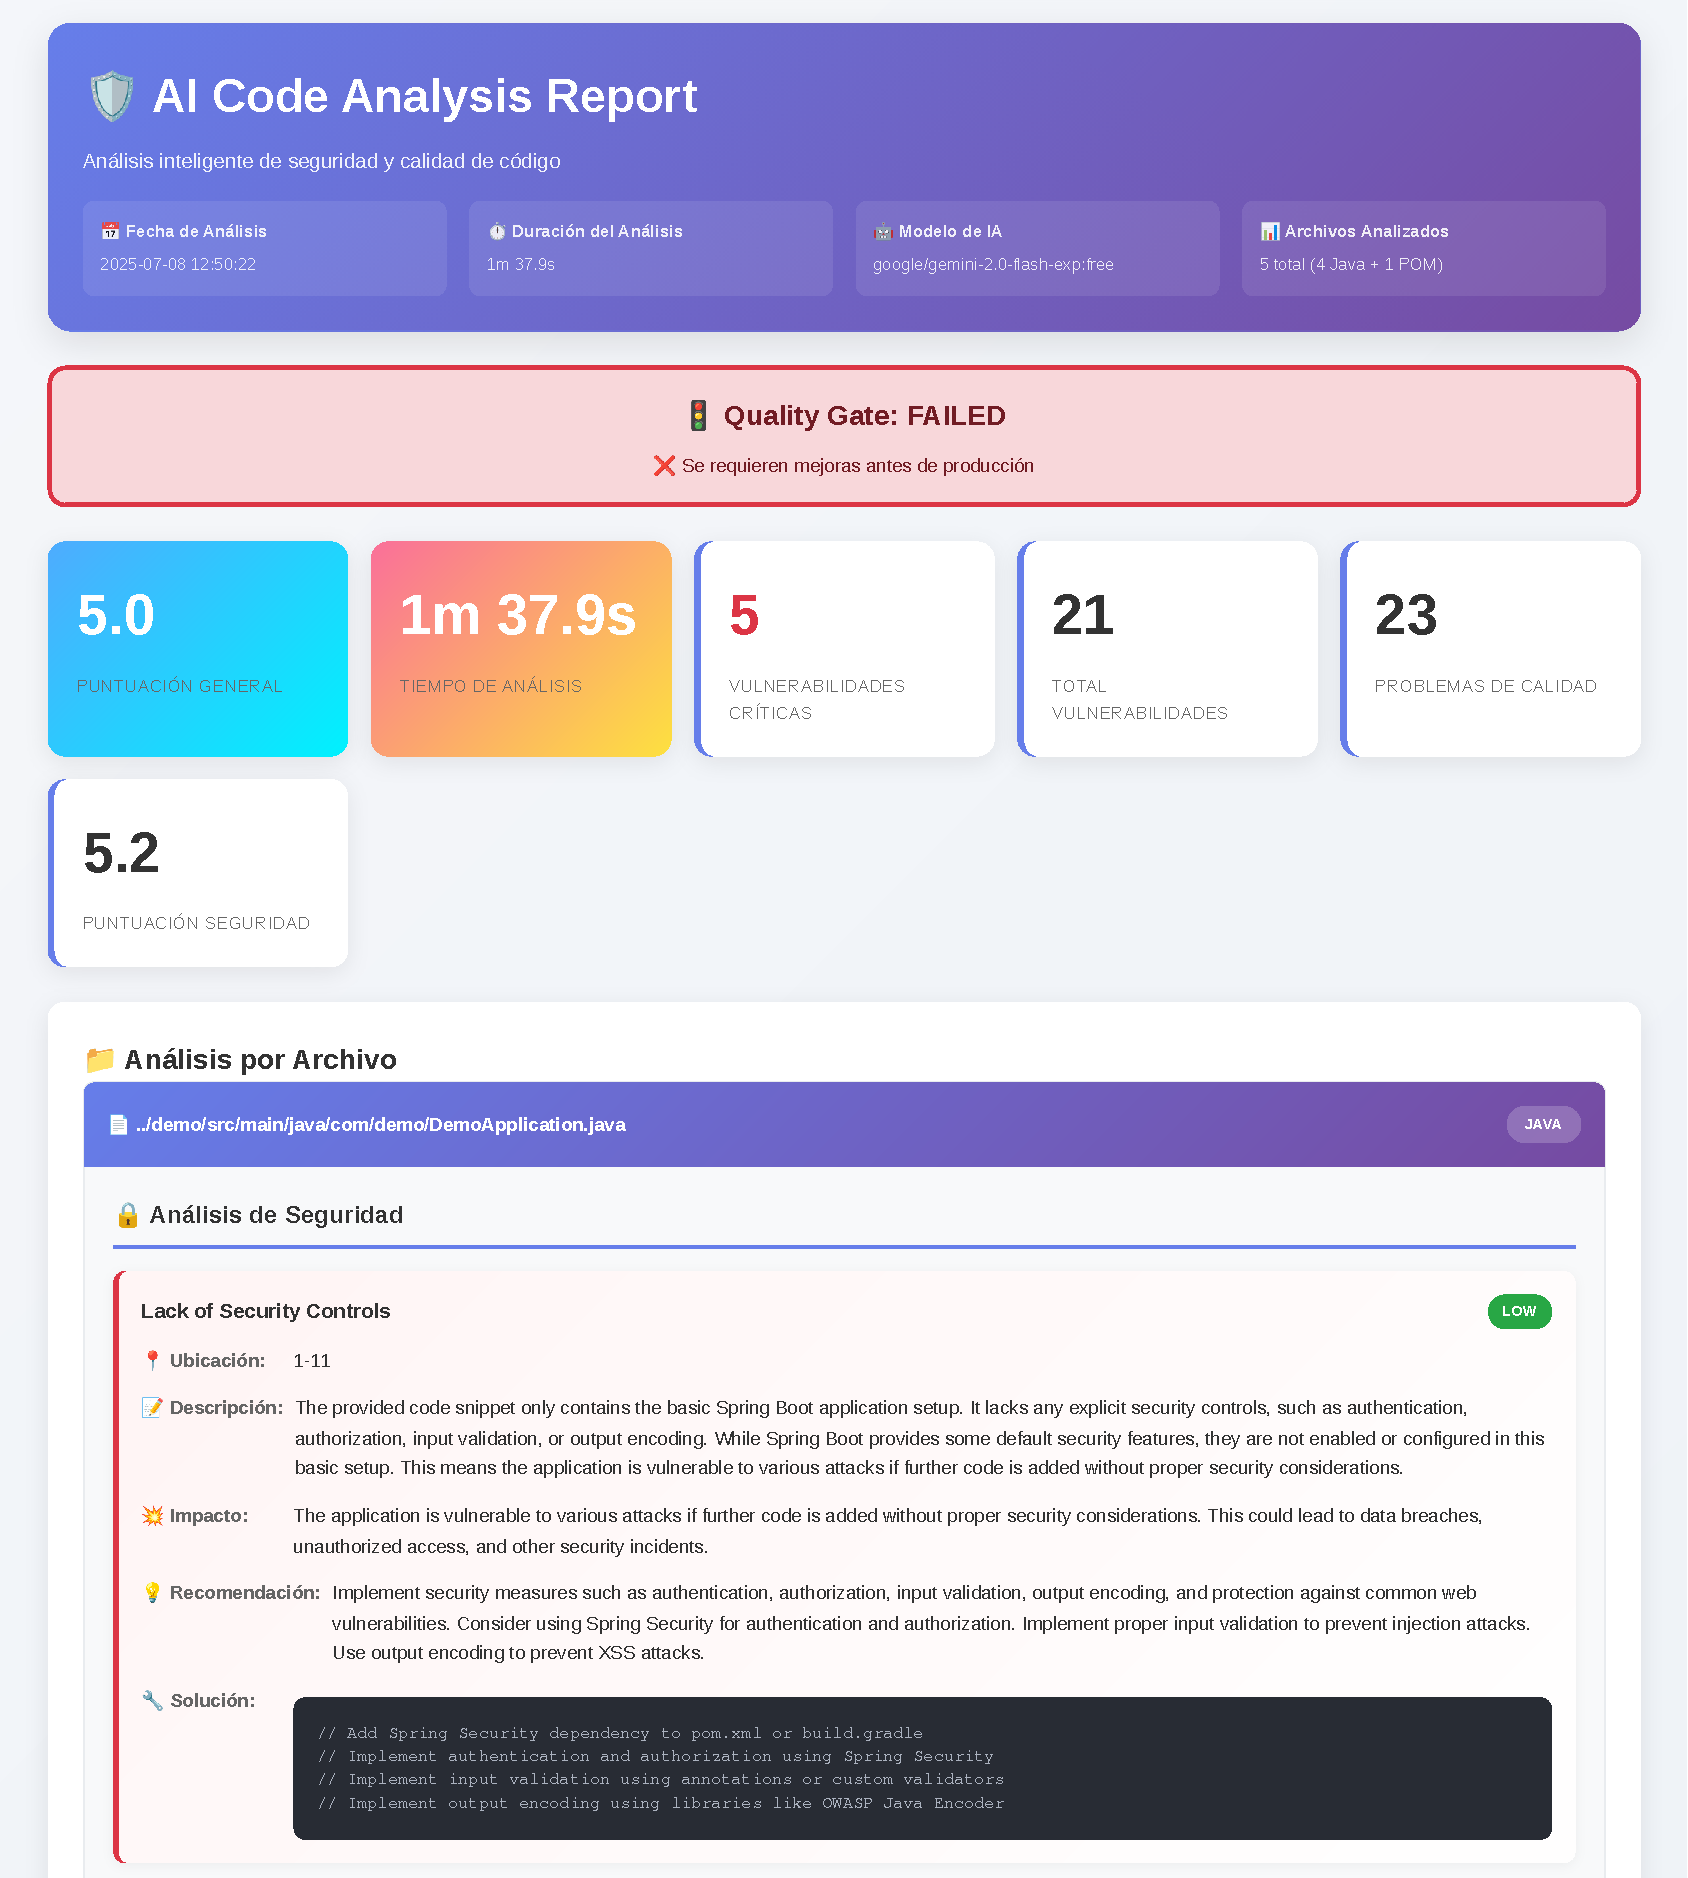
\includepdf[
    pages=-,
    width=\textwidth,
    height=\textheight,
    keepaspectratio,
    % Esta opción aplica el estilo 'plain' (solo número de página)
    % a CADA página del PDF insertado.
    pagecommand={\thispagestyle{plain}}
]{contenido/pdfs/ai-analysis-report.pdf}

    %--- Apéndices y bibliografia ---%
    %\cleardoublepage
\phantomsection
\addcontentsline{toc}{chapter}{Bibliografía}
\printbibliography

    %%\begin{appendices}
       % %Incluir aqui todos los apendices (carpeta contenido).
        %% --- INICIO DE LA SECCIÓN DE ANEXOS ---

% El comando \appendix cambia la numeración de los capítulos a letras (A, B, C, etc.)
\appendix

% Con \cleardoublepage o \clearpage aseguras que los anexos comiencen en una página nueva.
\cleardoublepage 

% Título principal de la sección de anexos
\chapter*{Anexos}
\addcontentsline{toc}{chapter}{Anexos} % Añade "Anexos" a la tabla de contenido


\chapter{Archivo Docker Compose}
\label{anexo:dockercompose}

\begin{lstlisting}[language=yaml, caption={Contenido del archivo docker-compose.yml para levantar el entorno.}, label={lst:docker-compose}]
services:
  jenkins:
    build: .
    image: ${IMAGE_NAME}
    container_name: ${CONTAINER_NAME}
    restart: always
    ports:
      - "8080:8080"
      - "50000:50000"
    volumes:
      - jenkins_data:/var/jenkins_home
      - /var/run/docker.sock:/var/run/docker.sock
    environment:
      - JENKINS_ADMIN_PASSWORD=${JENKINS_ADMIN_PASSWORD}
      - JAVA_OPTS=${JAVA_OPTS}
      - PIPELINE_NAME=${PIPELINE_NAME}
      - REPO_URL=${REPO_URL}
      - BRANCH=${BRANCH}
      - JENKINSFILE_PATH=${JENKINSFILE_PATH}

volumes:
  jenkins_data:
\end{lstlisting}

\chapter{Archivo Jenkinsfile}
\label{anexo:jenkinsfile}

\begin{lstlisting}[language=groovy, caption={Estructura completa del Jenkinsfile.}, label={lst:jenkinsfile}]
/**
 * =============================================================================
 * PIPELINE DE DEVSECOPS CON ANÁLISIS IA
 * =============================================================================
 * * Este pipeline implementa un ciclo de vida de CI/CD para una aplicación Java,
 * integrando la seguridad como un componente central a través de las siguientes fases:
 * * 1. Compilación y Pruebas Unitarias.
 * 2. Análisis Estático de Seguridad (SAST) con SpotBugs.
 * 3. Análisis Avanzado de Seguridad y Calidad con un modelo de IA.
 * 4. Quality Gate: Detención automática del pipeline si se encuentran vulnerabilidades críticas.
 * 5. Construcción y Despliegue de la aplicación como un contenedor Docker.
 * * =============================================================================
 */
pipeline {
    // Define que el pipeline puede ejecutarse en cualquier agente de Jenkins disponible.
    // Para entornos de producción, se recomienda usar etiquetas para seleccionar agentes específicos.
    agent any

    // --- Variables de Entorno Globales ---
    // Definen parámetros y rutas consistentes a lo largo de todo el pipeline.
    environment {
        // Directorio para almacenar todos los artefactos de análisis generados.
        SCAN_RESULTS_DIR = 'scan-results'
        // Nombre del proyecto, puede usarse para etiquetar artefactos o imágenes.
        PROJECT_NAME = 'demo'
        // Directorio del código fuente a analizar. Se usa una ruta absoluta para mayor robustez.
        JAVA_ANALYSIS_DIR    = "${env.WORKSPACE}/demo/src"
        // Límite de archivos a pasar al script de análisis de IA.
        MAX_FILES_TO_ANALYZE = '10'
    }
    
    // --- Etapas del Pipeline ---
    // Cada 'stage' representa una fase lógica y distinta del proceso de CI/CD.
    stages {

        // Etapa 1: Preparación y Compilación
        // Prepara el entorno, instala dependencias y compila la aplicación.
        stage('Compile & Prepare Environment') {
            steps {
                echo '>>> Stage: Compilando la aplicación y preparando el entorno...'
                
                // Verificación de versiones para diagnóstico.
                sh "java -version"
                sh "python3 --version"

                // Instala las dependencias de Python de forma idempotente.
                sh "pip3 install requests pathlib --break-system-packages || pip3 install requests pathlib || echo 'Dependencies already installed'"
                                
                // Crea el directorio de resultados si no existe.
                sh "mkdir -p ${SCAN_RESULTS_DIR}"
                
                // Entra al directorio del proyecto Java para ejecutar Maven.
                dir('demo') {
                    // Compila y empaqueta la aplicación. 
                    // -Dmaven.test.failure.ignore=true asegura que el pipeline continúe al análisis
                    // de seguridad incluso si las pruebas unitarias fallan, priorizando la seguridad.
                    sh "mvn -Dmaven.test.failure.ignore=true clean package"
                }
            }
        }

        // Etapa 2: Pruebas Unitarias
        // Analiza y publica los resultados de las pruebas unitarias.
        stage('Unit Test Analysis') {
            steps {
                echo '>>> Stage: Publicando resultados de pruebas unitarias...'
                
                // El paso 'junit' parsea los reportes XML y los integra en la UI de Jenkins,
                // mostrando tendencias, fallos y duración de las pruebas.
                junit 'demo/target/surefire-reports/*.xml'
            }
        }
        
        // Etapa 3: Análisis Estático de Seguridad (SAST)
        // Ejecuta herramientas de análisis estático en paralelo para optimizar el tiempo.
        stage('Static Analysis') {
            parallel {
                // Ejecuta SpotBugs para encontrar patrones de error comunes en el código Java.
                stage('SpotBugs SAST') {
                    steps {
                        dir('demo') {
                            script {
                                // El bloque try-catch añade resiliencia. Si SpotBugs falla,
                                // el pipeline no se detendrá, solo se registrará el error.
                                try {
                                    sh "mvn compile spotbugs:spotbugs"
                                    sh "cp target/spotbugsXml.xml ../${SCAN_RESULTS_DIR}/ || echo 'No SpotBugs report found'"
                                } catch (Exception e) {
                                    echo "SpotBugs analysis failed: ${e.getMessage()}"
                                    sh "echo '<BugCollection></BugCollection>' > ../${SCAN_RESULTS_DIR}/spotbugsXml.xml"
                                }
                            }
                        }
                    }
                }
                
                // Recopila los archivos fuente para la siguiente etapa.
                stage('Collect Source Files') {
                    steps {
                        script {
                            sh """
                                find ${JAVA_ANALYSIS_DIR} -name "*.java" -type f > ${SCAN_RESULTS_DIR}/java-files.txt
                                echo "Archivos Java encontrados para análisis:"
                                cat ${SCAN_RESULTS_DIR}/java-files.txt
                            """
                        }
                    }
                }
            }
        }
        
        // Etapa 4: Análisis con Inteligencia Artificial
        // Ejecuta el script de Python personalizado para un análisis de seguridad profundo.
        stage('AI-Powered Analysis') {
            steps {
                script {
                    // Copia el script de análisis al directorio de resultados para aislar la ejecución.
                    sh "cp demo/ai_code_analyzer.py ${SCAN_RESULTS_DIR}/"

                    // Ejecuta los siguientes pasos desde dentro del directorio de resultados.
                    dir(env.SCAN_RESULTS_DIR) {
                        // withCredentials es el mecanismo seguro de Jenkins para manejar secretos.
                        // Inyecta la credencial 'openrouter-api-key' en una variable de entorno
                        // temporal que solo existe dentro de este bloque.
                        withCredentials([string(credentialsId: 'openrouter-api-key', variable: 'OPENROUTER_API_KEY')]) {
                            sh """
                                echo "Iniciando análisis con IA..."
                                python3 ai_code_analyzer.py \\
                                    --directory ${JAVA_ANALYSIS_DIR} \\
                                    --max-files ${MAX_FILES_TO_ANALYZE}
                            """
                        }
                    }
                }
            }
        }    

        // Etapa 5: Quality Gate (Control de Calidad)
        // Punto de control que detiene el pipeline si no se cumplen las políticas de seguridad.
        stage('Quality Gate') {
            steps {
                script {
                    echo '>>> Stage: Verificando políticas de calidad y seguridad...'
                    def resultsFile = "${env.SCAN_RESULTS_DIR}/analysis-results.json"
                    
                    if (fileExists(resultsFile)) {
                        // Lee el archivo JSON generado por el script de IA.
                        def analysisResults = readJSON(file: resultsFile)
                        def highSeverityVulns = analysisResults.summary.high_severity_vulnerabilities
                        
                        echo "-> Vulnerabilidades de severidad ALTA encontradas: ${highSeverityVulns}"
                        
                        // --- Política de Seguridad: Cero Tolerancia para Vulnerabilidades Altas ---
                        if (highSeverityVulns > 0) {
                            // El paso 'error' detiene el pipeline inmediatamente y lo marca como FAILURE.
                            // Esto previene que código inseguro sea construido o desplegado.
                            error("QUALITY GATE FAILED: Se encontraron ${highSeverityVulns} vulnerabilidades de severidad ALTA. Abortando el pipeline.")
                        } else {
                            echo "QUALITY GATE PASSED: No se encontraron vulnerabilidades de severidad ALTA."
                        }
                        
                    } else {
                        // Si el archivo de resultados no existe, es un fallo crítico del proceso de análisis.
                        error("QUALITY GATE FAILED: No se encontró el archivo de resultados '${resultsFile}'. No se puede verificar la calidad.")
                    }
                }
            }
        }

        // Etapa 6: Construcción de Imagen Docker
        // Esta etapa solo se ejecuta si el Quality Gate fue superado.
        stage('Build Docker Image') {
            steps {
                echo '>>> Stage: Construyendo la imagen Docker de la aplicación...'
                script {
                    // El comando 'docker build' usa el Dockerfile de la aplicación.
                    // -f especifica la ruta del Dockerfile.
                    // -t etiqueta la imagen con un nombre y tag (ej: demo-app:latest).
                    // . define el contexto de construcción (el directorio actual).
                    sh 'docker build -f demo/Dockerfile -t demo-app .'
                }
            }
        }

        // Etapa 7: Despliegue en Entorno Local
        // Despliega la imagen construida como un contenedor local.
        stage('Deploy to Local Environment') {
            steps {
                echo '>>> Stage: Desplegando localmente con Docker...'
                
                // Detiene y elimina cualquier contenedor anterior con el mismo nombre.
                // '|| true' evita que el pipeline falle si el contenedor no existe.
                sh 'docker stop demo-app || true'
                sh 'docker rm demo-app || true'

                // Ejecuta el nuevo contenedor.
                // -d: modo detached (en segundo plano).
                // -p 8081:9090 mapea el puerto 9090 del contenedor al 8081 del host.
                // --name asigna un nombre al contenedor para fácil referencia.
                sh 'docker run -d -p 8081:9090 --name demo-app demo-app'
                
                echo '>>> El microservicio debería estar accesible en http://localhost:8081'
            }
        }
    }

    // --- Acciones Post-Ejecución ---
    // Se ejecutan al final del pipeline, sin importar el resultado de las etapas.
    post {
        // 'always' se ejecuta siempre, garantizando que los reportes y artefactos
        // siempre se publiquen, lo cual es crucial para la trazabilidad y el análisis de fallos.
        always {
            echo '>>> Post-execution: Publicando reportes y archivando artefactos...'
            
            // Publica los resultados de JUnit.
            junit(
                allowEmptyResults: true, 
                testResults: 'demo/target/surefire-reports/*.xml'
            )
            
            // Publica el reporte HTML del análisis de IA en la página del build.
            publishHTML([
                allowMissing: false,
                alwaysLinkToLastBuild: true,
                keepAll: true,
                reportDir: env.SCAN_RESULTS_DIR,
                reportFiles: 'ai-analysis-report.html',
                reportName: 'AI Security & Quality Report'
            ])
            
            // Archiva los reportes JSON y HTML como artefactos del build para su descarga.
            archiveArtifacts(
                artifacts: "${env.SCAN_RESULTS_DIR}/*.json, ${env.SCAN_RESULTS_DIR}/*.html",
                allowEmptyArchive: true
            )
        }
        
        // Bloques para notificaciones contextuales (ej. Slack, Email, Teams).
        success {
            echo 'Pipeline completado exitosamente!'
        }
        failure {
            echo 'Pipeline falló! Revisar los logs.'
        }
        unstable {
            echo 'Pipeline completado con advertencias (inestable).'
        }
    }
}
\end{lstlisting}


\chapter{Archivo ai\_analyzer.py}
\label{anexo:ai_analyzer}
\begin{lstlisting}[language=python, caption={Contenido completo del script ai\_analyzer.py.}, label={lst:python_script}]
import json
import os
import requests
import sys
import argparse
from pathlib import Path
from datetime import datetime
import hashlib

class OpenRouterAnalyzer:
    def __init__(self):
        # Leer la API key desde variable de entorno
        self.api_key = os.getenv('OPENROUTER_API_KEY')
        
        # Verificar que la API key esté disponible
        if not self.api_key:
            print("ERROR: La variable de entorno OPENROUTER_API_KEY no está configurada.")
            print("Variables de entorno disponibles:")
            for key, value in os.environ.items():
                if 'OPENROUTER' in key.upper():
                    print(f"  {key}: {value[:10]}...")
            raise ValueError("OPENROUTER_API_KEY no encontrada en las variables de entorno")
        
        print(f"API Key cargada correctamente: {self.api_key[:10]}...")
        
        self.base_url = "https://openrouter.ai/api/v1"
        self.headers = {
            "Authorization": f"Bearer {self.api_key}",
            "Content-Type": "application/json",
            "HTTP-Referer": "http://localhost:8080",
            "X-Title": "Jenkins CI/CD Security Scanner"
        }
        
    def analyze_code_security(self, code_content, filename):
        """Analizar código Java para vulnerabilidades de seguridad"""
        prompt = f"""
Actúa como un experto en seguridad de aplicaciones Java. Analiza el siguiente código fuente para identificar vulnerabilidades de seguridad:

Archivo: {filename}

Busca específicamente:
1. Inyección SQL
2. Cross-Site Scripting (XSS)
3. Problemas de autenticación/autorización
4. Validación de entrada insuficiente
5. Exposición de información sensible
6. Vulnerabilidades de deserialización
7. Uso inseguro de criptografía
8. Path traversal
9. Command injection
10. Problemas de gestión de sesiones

Código a analizar:
```java
{code_content}
```

Responde en formato JSON con la siguiente estructura:
{{
    "vulnerabilities": [
        {{
            "type": "tipo de vulnerabilidad",
            "severity": "HIGH|MEDIUM|LOW",
            "line": "número de línea aproximado",
            "description": "descripción detallada",
            "recommendation": "cómo solucionarlo",
            "code_correction_suggested": "codigo para solucionar la vulnerabilidad",
            "cwe_id": "CWE-XXX si aplica",
            "impact": "impacto potencial de la vulnerabilidad"
        }}
    ],
    "security_score": "puntuación del 0-10",
    "summary": "resumen ejecutivo de los hallazgos"
}}
        """
        
        return self._call_api(prompt, "security")
    
    def analyze_code_quality(self, code_content, filename):
        """Analizar calidad del código Java"""
        prompt = f"""
Actúa como un experto en calidad de código Java. Analiza el siguiente código para identificar problemas de calidad:

Archivo: {filename}

Evalúa:
1. Code smells y anti-patrones
2. Complejidad ciclomática alta
3. Duplicación de código
4. Problemas de mantenibilidad
5. Violaciones de principios SOLID
6. Uso inadecuado de patrones de diseño
7. Gestión de excepciones
8. Nomenclatura y convenciones
9. Eficiencia y rendimiento
10. Cobertura y calidad de comentarios

Código a analizar:
```java
{code_content}
```

Responde en formato JSON:
{{
    "quality_issues": [
        {{
            "type": "tipo de problema",
            "severity": "HIGH|MEDIUM|LOW",
            "line": "número de línea aproximado",
            "description": "descripción del problema",
            "recommendation": "mejora sugerida",
            "code_correction_suggested": "codigo para solucionar el problema",
            "category": "Maintainability|Reliability|Performance|Documentation",
            "effort": "tiempo estimado para solucionar (minutos)"
        }}
    ],
    "quality_score": "puntuación del 0-10",
    "maintainability_index": "índice de mantenibilidad",
    "complexity_score": "puntuación de complejidad",
    "technical_debt": "deuda técnica estimada en minutos"
}}
        """
        
        return self._call_api(prompt, "quality")
    
    def _call_api(self, prompt, analysis_type):
        """Llamar a la API de OpenRouter"""
        payload = {
            "model": "deepseek/deepseek-chat",
            "messages": [
                {
                    "role": "user", 
                    "content": prompt
                }
            ],
            "temperature": 0.1,
            "max_tokens": 4000
        }
        
        try:
            response = requests.post(
                f"{self.base_url}/chat/completions",
                headers=self.headers,
                json=payload,
                timeout=60
            )
            # --- INICIO DE LÍNEAS DE DEPURACIÓN A AGREGAR ---
            print(f"--- DEBUG: Respuesta de la API para '{analysis_type}' ---")
            print(f"Status Code: {response.status_code}")
            print(f"Response Body (Raw): {response.text}")
            print("-------------------------------------------------")
            # --- FIN DE LÍNEAS DE DEPURACIÓN A AGREGAR ---
            if response.status_code == 200:
                result = response.json()
                content = result["choices"][0]["message"]["content"]
                
                # Intentar extraer JSON del contenido
                try:
                    # Buscar JSON en el contenido
                    start = content.find("{")
                    end = content.rfind("}") + 1
                    if start != -1 and end > start:
                        json_content = content[start:end]
                        return json.loads(json_content)
                    else:
                        return {"error": "No se pudo extraer JSON válido", "raw_content": content}
                except json.JSONDecodeError:
                    return {"error": "JSON inválido", "raw_content": content}
            else:
                return {"error": f"API Error: {response.status_code}", "message": response.text}
                
        except Exception as e:
            return {"error": f"Exception: {str(e)}"}
    
    def calculate_overall_score(self, ai_results):
        """Calcular puntuación general del proyecto"""
        total_security_score = 0
        total_quality_score = 0
        valid_files = 0
        
        for result in ai_results.values():
            if isinstance(result, dict) and not result.get('error'):
                if 'security_score' in result:
                    try:
                        total_security_score += float(result['security_score'])
                        valid_files += 1
                    except (ValueError, TypeError):
                        pass
                if 'quality_score' in result:
                    try:
                        total_quality_score += float(result['quality_score'])
                    except (ValueError, TypeError):
                        pass
        
        if valid_files > 0:
            avg_security_score = total_security_score / valid_files
            avg_quality_score = total_quality_score / valid_files
            overall_score = (avg_security_score + avg_quality_score) / 2
            return overall_score, avg_security_score, avg_quality_score
        
        return 0, 0, 0
    
    def generate_report(self, ai_results):
        """Generar reporte HTML comprensivo y moderno"""
        
        # Calcular estadísticas generales
        total_vulnerabilities = sum(len(result.get('vulnerabilities', [])) for result in ai_results.values() if isinstance(result, dict))
        total_quality_issues = sum(len(result.get('quality_issues', [])) for result in ai_results.values() if isinstance(result, dict))
        
        # Contar por severidad
        high_severity_vulns = sum(1 for result in ai_results.values() if isinstance(result, dict) 
                                 for vuln in result.get('vulnerabilities', []) 
                                 if vuln.get('severity') == 'HIGH')
        
        medium_severity_vulns = sum(1 for result in ai_results.values() if isinstance(result, dict) 
                                   for vuln in result.get('vulnerabilities', []) 
                                   if vuln.get('severity') == 'MEDIUM')
        
        low_severity_vulns = sum(1 for result in ai_results.values() if isinstance(result, dict) 
                                for vuln in result.get('vulnerabilities', []) 
                                if vuln.get('severity') == 'LOW')
        
        # Calcular puntuación general
        overall_score, avg_security_score, avg_quality_score = self.calculate_overall_score(ai_results)
        
        # Determinar el estado del quality gate
        quality_gate_status = "PASSED" #if high_severity_vulns == 0 and overall_score >= 7 else "FAILED"
        
        # Generar timestamp
        timestamp = datetime.now().strftime("%Y-%m-%d %H:%M:%S")
        
        html_content = f"""
<!DOCTYPE html>
<html lang="es">
<head>
    <meta charset="UTF-8">
    <meta name="viewport" content="width=device-width, initial-scale=1.0">
    <title>AI Code Analysis Report</title>
    <style>
        * {{
            margin: 0;
            padding: 0;
            box-sizing: border-box;
        }}
        
        body {{
            font-family: -apple-system, BlinkMacSystemFont, 'Segoe UI', Roboto, Oxygen, Ubuntu, Cantarell, sans-serif;
            line-height: 1.6;
            color: #333;
            background: linear-gradient(135deg, #f5f7fa 0%, #c3cfe2 100%);
            min-height: 100vh;
        }}
        
        .container {{
            max-width: 1400px;
            margin: 0 auto;
            padding: 20px;
        }}
        
        .header {{
            background: linear-gradient(135deg, #667eea 0%, #764ba2 100%);
            color: white;
            padding: 30px;
            border-radius: 20px;
            margin-bottom: 30px;
            box-shadow: 0 10px 30px rgba(0,0,0,0.1);
        }}
        
        .header h1 {{
            font-size: 2.5rem;
            margin-bottom: 10px;
            font-weight: 700;
        }}
        
        .header .subtitle {{
            font-size: 1.1rem;
            opacity: 0.9;
            margin-bottom: 20px;
        }}
        
        .meta-info {{
            display: flex;
            gap: 30px;
            font-size: 0.9rem;
            opacity: 0.8;
        }}
        
        .quality-gate {{
            background: {'#d4edda' if quality_gate_status == 'PASSED' else '#f8d7da'};
            color: {'#155724' if quality_gate_status == 'PASSED' else '#721c24'};
            padding: 20px;
            border-radius: 15px;
            margin-bottom: 30px;
            border: 3px solid {'#28a745' if quality_gate_status == 'PASSED' else '#dc3545'};
            text-align: center;
        }}
        
        .quality-gate h2 {{
            font-size: 1.5rem;
            margin-bottom: 10px;
        }}
        
        .metrics-grid {{
            display: grid;
            grid-template-columns: repeat(auto-fit, minmax(250px, 1fr));
            gap: 20px;
            margin-bottom: 30px;
        }}
        
        .metric-card {{
            background: white;
            padding: 25px;
            border-radius: 15px;
            box-shadow: 0 5px 20px rgba(0,0,0,0.08);
            border-left: 5px solid #667eea;
            transition: transform 0.3s ease;
        }}
        
        .metric-card:hover {{
            transform: translateY(-5px);
        }}
        
        .metric-number {{
            font-size: 3rem;
            font-weight: 700;
            margin-bottom: 10px;
        }}
        
        .metric-label {{
            font-size: 0.9rem;
            color: #666;
            text-transform: uppercase;
            letter-spacing: 0.5px;
        }}
        
        .score-card {{
            background: linear-gradient(135deg, #4facfe 0%, #00f2fe 100%);
            color: white;
            border-left: none;
        }}
        
        .severity-high {{ color: #dc3545; }}
        .severity-medium {{ color: #fd7e14; }}
        .severity-low {{ color: #28a745; }}
        
        .files-section {{
            background: white;
            border-radius: 15px;
            padding: 30px;
            margin-bottom: 30px;
            box-shadow: 0 5px 20px rgba(0,0,0,0.08);
        }}
        
        .file-card {{
            background: #f8f9fa;
            border-radius: 10px;
            margin-bottom: 30px;
            overflow: hidden;
            border: 1px solid #e9ecef;
        }}
        
        .file-header {{
            background: linear-gradient(135deg, #667eea 0%, #764ba2 100%);
            color: white;
            padding: 20px;
            font-weight: 600;
        }}
        
        .file-content {{
            padding: 25px;
        }}
        
        .analysis-section {{
            margin-bottom: 30px;
        }}
        
        .section-title {{
            font-size: 1.3rem;
            margin-bottom: 20px;
            color: #333;
            border-bottom: 2px solid #667eea;
            padding-bottom: 10px;
        }}
        
        .issue-card {{
            background: white;
            border-radius: 10px;
            padding: 20px;
            margin-bottom: 15px;
            border-left: 4px solid #667eea;
            box-shadow: 0 2px 10px rgba(0,0,0,0.05);
        }}
        
        .vulnerability-card {{
            border-left-color: #dc3545;
            background: linear-gradient(135deg, #fff5f5 0%, #ffffff 100%);
        }}
        
        .quality-card {{
            border-left-color: #007bff;
            background: linear-gradient(135deg, #f0f8ff 0%, #ffffff 100%);
        }}
        
        .issue-header {{
            display: flex;
            justify-content: space-between;
            align-items: center;
            margin-bottom: 15px;
        }}
        
        .issue-title {{
            font-size: 1.1rem;
            font-weight: 600;
            color: #333;
        }}
        
        .severity-badge {{
            padding: 4px 12px;
            border-radius: 20px;
            font-size: 0.8rem;
            font-weight: 600;
            text-transform: uppercase;
        }}
        
        .severity-high-bg {{
            background: #dc3545;
            color: white;
        }}
        
        .severity-medium-bg {{
            background: #fd7e14;
            color: white;
        }}
        
        .severity-low-bg {{
            background: #28a745;
            color: white;
        }}
        
        .issue-details {{
            display: grid;
            gap: 15px;
        }}
        
        .detail-item {{
            display: flex;
            align-items: flex-start;
            gap: 10px;
        }}
        
        .detail-label {{
            font-weight: 600;
            color: #666;
            min-width: 100px;
        }}
        
        .detail-content {{
            flex: 1;
        }}
        
        .code-block {{
            background: #282c34;
            color: #abb2bf;
            padding: 20px;
            border-radius: 10px;
            overflow-x: auto;
            margin-top: 10px;
            font-family: 'Consolas', 'Monaco', 'Courier New', monospace;
            font-size: 0.9rem;
            line-height: 1.4;
        }}
        
        .code-block pre {{
            margin: 0;
            white-space: pre-wrap;
            word-wrap: break-word;
        }}
        
        .no-issues {{
            text-align: center;
            color: #28a745;
            font-size: 1.1rem;
            padding: 40px;
            background: linear-gradient(135deg, #d4edda 0%, #ffffff 100%);
            border-radius: 10px;
            border: 2px solid #28a745;
        }}
        
        .footer {{
            text-align: center;
            padding: 20px;
            color: #666;
            font-size: 0.9rem;
        }}
        
        @media (max-width: 768px) {{
            .metrics-grid {{
                grid-template-columns: 1fr;
            }}
            
            .header h1 {{
                font-size: 2rem;
            }}
            
            .meta-info {{
                flex-direction: column;
                gap: 10px;
            }}
        }}
    </style>
</head>
<body>
    <div class="container">
        <div class="header">
            <h1>AI Code Analysis Report</h1>
            <div class="subtitle">Análisis inteligente de seguridad y calidad de código</div>
            <div class="meta-info">
                <div>Generado: {timestamp}</div>
                <div>Archivos analizados: {len(ai_results)}</div>
                <div>Powered by AI</div>
            </div>
        </div>
        
        <div class="quality-gate">
            <h2>Quality Gate: {quality_gate_status}</h2>
            <p>{'Tu código cumple con los estándares de calidad' if quality_gate_status == 'PASSED' else 'Se requieren mejoras antes de producción'}</p>
        </div>
        
        <div class="metrics-grid">
            <div class="metric-card score-card">
                <div class="metric-number">{overall_score:.1f}</div>
                <div class="metric-label">Puntuación General</div>
            </div>
            
            <div class="metric-card">
                <div class="metric-number severity-high">{high_severity_vulns}</div>
                <div class="metric-label">Vulnerabilidades Críticas</div>
            </div>
            
            <div class="metric-card">
                <div class="metric-number">{total_vulnerabilities}</div>
                <div class="metric-label">Total Vulnerabilidades</div>
            </div>
            
            <div class="metric-card">
                <div class="metric-number">{total_quality_issues}</div>
                <div class="metric-label">Problemas de Calidad</div>
            </div>
            
            <div class="metric-card">
                <div class="metric-number">{avg_security_score:.1f}</div>
                <div class="metric-label">Puntuación Seguridad</div>
            </div>
            
            <div class="metric-card">
                <div class="metric-number">{avg_quality_score:.1f}</div>
                <div class="metric-label">Puntuación Calidad</div>
            </div>
        </div>
        
        <div class="files-section">
            <h2>Análisis por Archivo</h2>
"""
        
        # Agregar resultados por archivo
        for filename, results in ai_results.items():
            if isinstance(results, dict):
                html_content += f"""
            <div class="file-card">
                <div class="file-header">
                    <div>{filename}</div>
                </div>
                <div class="file-content">
"""
                
                # Análisis de Seguridad
                html_content += """
                    <div class="analysis-section">
                        <h3 class="section-title">Análisis de Seguridad</h3>
"""
                
                vulnerabilities = results.get('vulnerabilities', [])
                if vulnerabilities:
                    for vuln in vulnerabilities:
                        severity = vuln.get('severity', 'LOW')
                        html_content += f"""
                        <div class="issue-card vulnerability-card">
                            <div class="issue-header">
                                <div class="issue-title">{vuln.get('type', 'Unknown Vulnerability')}</div>
                                <div class="severity-badge severity-{severity.lower()}-bg">{severity}</div>
                            </div>
                            <div class="issue-details">
                                <div class="detail-item">
                                    <div class="detail-label">Línea:</div>
                                    <div class="detail-content">{vuln.get('line', 'N/A')}</div>
                                </div>
                                <div class="detail-item">
                                    <div class="detail-label">Descripción:</div>
                                    <div class="detail-content">{vuln.get('description', 'N/A')}</div>
                                </div>
                                <div class="detail-item">
                                    <div class="detail-label">Recomendación:</div>
                                    <div class="detail-content">{vuln.get('recommendation', 'N/A')}</div>
                                </div>
                                <div class="detail-item">
                                    <div class="detail-label">Solución:</div>
                                    <div class="detail-content">
                                        <div class="code-block">
                                            <pre>{vuln.get('code_correction_suggested', 'N/A')}</pre>
                                        </div>
                                    </div>
                                </div>
                            </div>
                        </div>
"""
                else:
                    html_content += """
                        <div class="no-issues">
                            No se encontraron vulnerabilidades de seguridad
                        </div>
"""
                
                html_content += """
                    </div>
"""
                
                # Análisis de Calidad
                html_content += """
                    <div class="analysis-section">
                        <h3 class="section-title">⚡ Análisis de Calidad</h3>
"""
                
                quality_issues = results.get('quality_issues', [])
                if quality_issues:
                    for issue in quality_issues:
                        severity = issue.get('severity', 'LOW')
                        html_content += f"""
                        <div class="issue-card quality-card">
                            <div class="issue-header">
                                <div class="issue-title">{issue.get('type', 'Unknown Issue')}</div>
                                <div class="severity-badge severity-{severity.lower()}-bg">{severity}</div>
                            </div>
                            <div class="issue-details">
                                <div class="detail-item">
                                    <div class="detail-label"> Línea:</div>
                                    <div class="detail-content">{issue.get('line', 'N/A')}</div>
                                </div>
                                <div class="detail-item">
                                    <div class="detail-label">Descripción:</div>
                                    <div class="detail-content">{issue.get('description', 'N/A')}</div>
                                </div>
                                <div class="detail-item">
                                    <div class="detail-label">Recomendación:</div>
                                    <div class="detail-content">{issue.get('recommendation', 'N/A')}</div>
                                </div>
                                <div class="detail-item">
                                    <div class="detail-label">Solución:</div>
                                    <div class="detail-content">
                                        <div class="code-block">
                                            <pre>{issue.get('code_correction_suggested', 'N/A')}</pre>
                                        </div>
                                    </div>
                                </div>
                            </div>
                        </div>
"""
                else:
                    html_content += """
                        <div class="no-issues">
                            No se encontraron problemas significativos de calidad
                        </div>
"""
                
                html_content += """
                    </div>
                </div>
            </div>
"""
        
        html_content += """
        </div>
        
        <div class="footer">
            <p>Reporte generado automáticamente por AI Code Analyzer</p>
            <p>Para más información sobre las vulnerabilidades, consulta OWASP Top 10 y CWE</p>
        </div>
    </div>
</body>
</html>
"""
        
        # Guardar archivo HTML
        with open("ai-analysis-report.html", "w", encoding="utf-8") as f:
            f.write(html_content)
        
        # También generar JSON para quality gates
        report_json = {
            "timestamp": timestamp,
            "overall_score": overall_score,
            "security_score": avg_security_score,
            "quality_score": avg_quality_score,
            "quality_gate_status": quality_gate_status,
            "summary": {
                "total_vulnerabilities": total_vulnerabilities,
                "high_severity_vulnerabilities": high_severity_vulns,
                "medium_severity_vulnerabilities": medium_severity_vulns,
                "low_severity_vulnerabilities": low_severity_vulns,
                "total_quality_issues": total_quality_issues,
                "files_analyzed": len(ai_results)
            },
            "detailed_results": ai_results
        }
        
        with open("analysis-results.json", "w", encoding="utf-8") as f:
            json.dump(report_json, f, indent=2, ensure_ascii=False)

def find_java_files(directory):
    """Buscar archivos Java en un directorio"""
    directory_path = Path(directory)
    
    if not directory_path.exists():
        print(f"El directorio {directory} no existe")
        return []
    
    if not directory_path.is_dir():
        print(f"{directory} no es un directorio válido")
        return []
    
    java_files = list(directory_path.rglob("*.java"))
    print(f"Buscando en: {directory_path.absolute()}")
    print(f"☕ Archivos Java encontrados: {len(java_files)}")
    
    return java_files

def get_analysis_directory():
    """Obtener el directorio a analizar desde argumentos o variables de entorno"""
    
    # Prioridad 1: Argumento de línea de comandos
    parser = argparse.ArgumentParser(description='Analizador de código Java con IA')
    parser.add_argument('--directory', '-d', 
                       help='Directorio a analizar (por defecto: busca en directorio actual)')
    parser.add_argument('--max-files', '-m', type=int, default=5,
                       help='Número máximo de archivos a analizar (por defecto: 5)')
    
    args = parser.parse_args()
    
    # Prioridad 2: Variable de entorno
    env_directory = os.getenv('JAVA_ANALYSIS_DIR')
    
    # Prioridad 3: Directorio por defecto
    if args.directory:
        analysis_dir = args.directory
        print(f"Directorio especificado por argumento: {analysis_dir}")
    elif env_directory:
        analysis_dir = env_directory
        print(f"Directorio especificado por variable de entorno: {analysis_dir}")
    else:
        # Buscar en directorio actual y subdirectorios
        analysis_dir = "."
        print(f"Usando directorio por defecto: {Path('.').absolute()}")
    
    return analysis_dir, args.max_files

def main():
    # Obtener y mostrar el directorio actual
    current_directory = Path.cwd()
    print(f"Directorio actual: {current_directory}")
    
    # Listar archivos en el directorio actual
    print("\nArchivos en el directorio actual:")
    for file in current_directory.iterdir():
        print(f"- {file.name}")
    
    analyzer = OpenRouterAnalyzer()

    # Obtener directorio a analizar
    analysis_directory, max_files = get_analysis_directory()
    
    # Buscar archivos Java
    print(f"\nBuscando archivos Java en: {analysis_directory}")
    java_files = find_java_files(analysis_directory)
    
    if not java_files:
        print(f"No se encontraron archivos Java en {analysis_directory}")
        print("Asegúrate de que el directorio contenga archivos .java")
        
        # Mostrar estructura de directorios para debugging
        analysis_path = Path(analysis_directory)
        if analysis_path.exists():
            print(f"\nEstructura del directorio {analysis_directory}:")
            for item in analysis_path.rglob("*"):
                if item.is_file():
                    print(f"  - {item.relative_to(analysis_path)}")
        
        sys.exit(1)
    
    # Limitar número de archivos a analizar
    files_to_analyze = java_files[:max_files]
    if len(java_files) > max_files:
        print(f"Limitando análisis a {max_files} archivos de {len(java_files)} encontrados")
    
    print(f"\nAnalizando {len(files_to_analyze)} archivos Java con IA...")
    
    ai_results = {}
    
    for java_file in files_to_analyze:
        try:
            with open(java_file, 'r', encoding='utf-8') as f:
                code_content = f.read()
                
            if len(code_content.strip()) == 0:
                continue
                
            print(f"Analizando: {java_file}")
            
            # Análisis de seguridad
            security_result = analyzer.analyze_code_security(code_content, str(java_file))
            
            # Análisis de calidad
            quality_result = analyzer.analyze_code_quality(code_content, str(java_file))
            
            # Combinar resultados
            combined_result = {}
            if isinstance(security_result, dict):
                combined_result.update(security_result)
            if isinstance(quality_result, dict):
                combined_result.update(quality_result)
            
            ai_results[str(java_file)] = combined_result
            
        except Exception as e:
            print(f"Error analizando {java_file}: {e}")
            ai_results[str(java_file)] = {"error": str(e)}
    
    # Generar reporte
    analyzer.generate_report(ai_results)
    
    print("Análisis completado. Reportes generados:")
    print("- ai-analysis-report.html")
    print("- analysis-results.json")

if __name__ == "__main__":
    main()
\end{lstlisting}


\chapter{Reporte de vulnerabilidades mediante IA}
\label{anexo:ai-analysis-report}

% Este comando restaura el estilo de página por defecto (con numeración)
% para la página donde comienza el anexo.
\thispagestyle{plain}

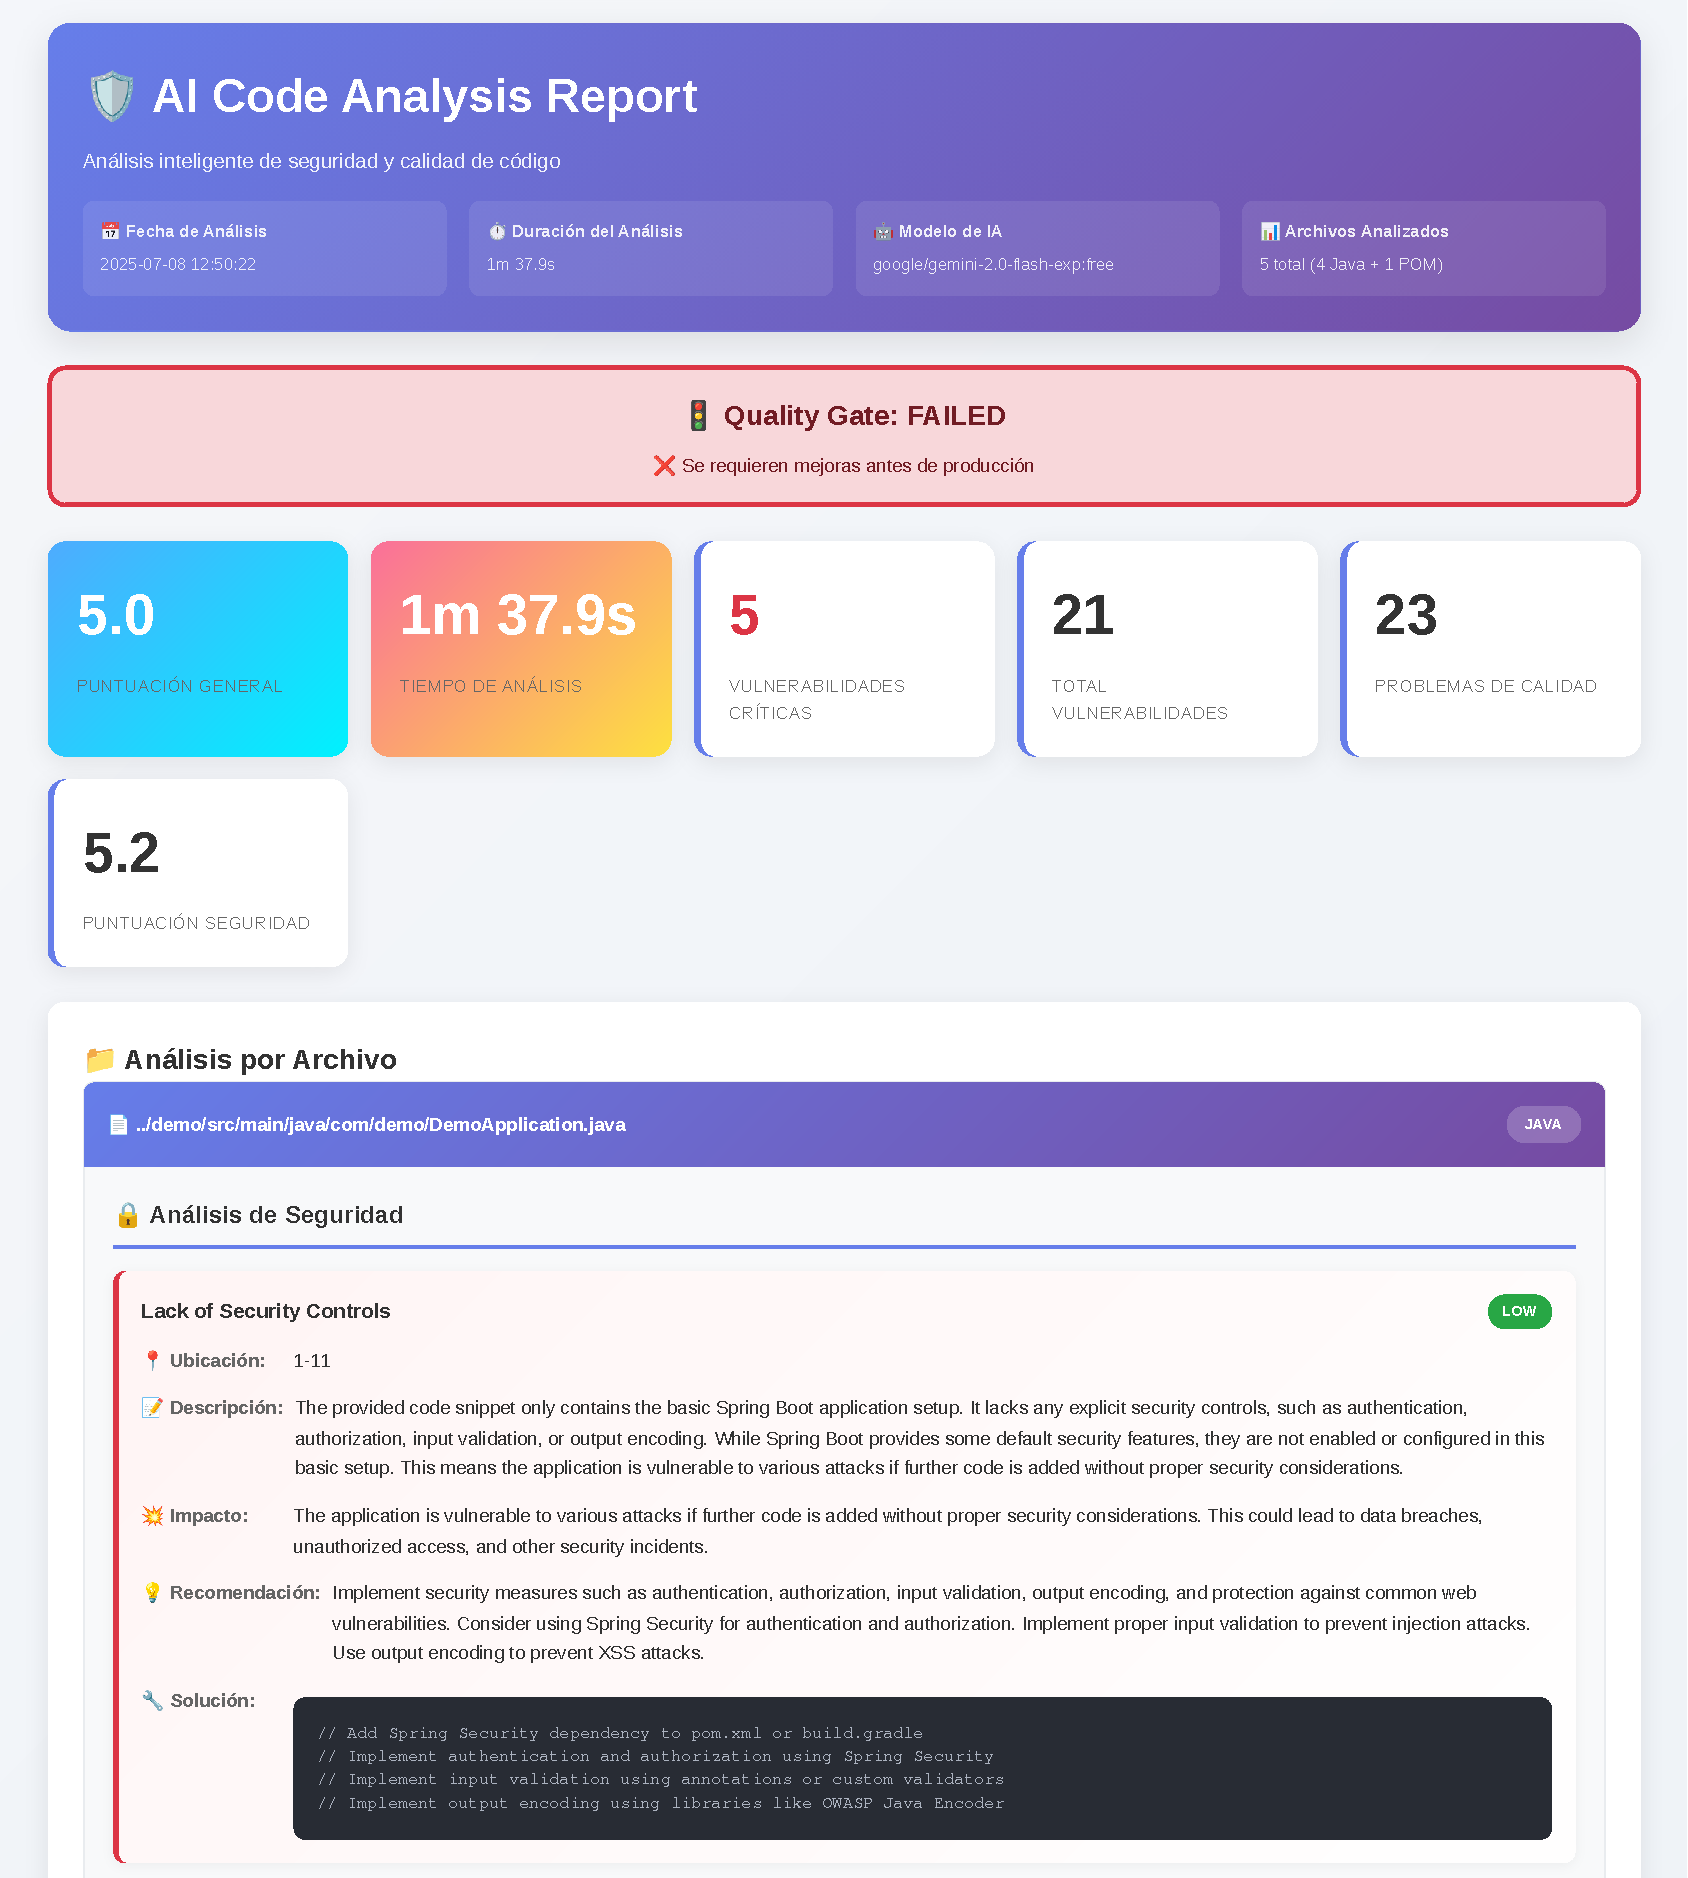
\includepdf[
    pages=-,
    width=\textwidth,
    height=\textheight,
    keepaspectratio,
    % Esta opción aplica el estilo 'plain' (solo número de página)
    % a CADA página del PDF insertado.
    pagecommand={\thispagestyle{plain}}
]{contenido/pdfs/ai-analysis-report.pdf}
        %\chapter{Etiam posuere laoreet}\label{app:two}
Maecenas faucibus nisl ut libero feugiat feugiat. Nam suscipit elementum lorem eget rutrum. Duis consequat tincidunt diam, quis hendrerit velit. Duis aliquam turpis suscipit leo sodales dignissim. Ut vulputate lacus sit amet eros eleifend, non tristique sem facilisis. Vestibulum vulputate sapien ut viverra mattis. Aenean sit amet ex magna. Duis sit amet felis a ante eleifend accumsan sed sodales tortor. Fusce hendrerit rutrum dictum. Vestibulum purus lectus, gravida vel fermentum id, rutrum ut ipsum. Morbi aliquam nulla sed venenatis eleifend. Fusce dictum ligula in mi bibendum volutpat. Morbi egestas ut lacus et iaculis. Cras tincidunt diam in urna dapibus faucibus. Nulla facilisi. Nam suscipit semper felis interdum ullamcorper.\par

Cras non est dignissim ipsum tempor faucibus. Proin varius felis nec augue accumsan congue. Aenean pulvinar a elit quis imperdiet. Cras auctor, ante vel pellentesque porta, eros magna volutpat tortor, eu eleifend augue erat sit amet elit. Nulla eu ex ac mi efficitur ultricies. In metus lectus, egestas vitae odio sit amet, faucibus feugiat lectus. Etiam posuere laoreet augue ut vestibulum. Vestibulum eget eros in leo luctus gravida. Fusce varius leo a ultrices tempor. Sed mattis, tortor ut imperdiet finibus, nunc erat elementum massa, sed facilisis sem felis nec risus. Morbi non vulputate purus, a efficitur ipsum. Aliquam fermentum tincidunt libero ac eleifend. Curabitur posuere, lorem ut accumsan fermentum, justo sem pulvinar urna, quis varius libero orci eu nisi. Morbi pharetra, magna viverra imperdiet molestie, purus velit molestie nisl, vitae porttitor purus nunc sed elit. 
    %\end{appendices}
\end{document}
